\documentclass[12pt]{article}
\usepackage{fullpage}
\usepackage{multirow}
\usepackage{graphicx}
\usepackage[sort&compress]{natbib}
\usepackage{amssymb, amsmath, amsthm}
\usepackage[breaklinks=true]{hyperref}
\hypersetup{
    colorlinks,
    citecolor= blue,
    filecolor= blue,
    linkcolor= blue,
    urlcolor= blue
}

\usepackage{setspace}
\usepackage{tikz}
\usetikzlibrary{patterns,arrows,decorations.pathreplacing}
\usepackage{subcaption}
\usepackage{booktabs}
\usepackage{multicol}
\usepackage{rotating}
\usepackage{tabularx}
\usepackage[normalem]{ulem}

\usepackage{siunitx}
\sisetup{group-separator={,},group-minimum-digits=3}

\usepackage[hang,flushmargin]{footmisc}

\newcommand{\insitu}{\textit{in situ} }
\newcommand{\SGER}{\textit{SGER} }
\newcommand{\CCIR}{\textit{CCIR} }

\newcommand{\co}{\text{CO$_2$ }}
\newcommand{\coe}{\text{CO$_2$e }}

%%%%%%%%%%



% FOR COMMENTING:
\usepackage{comment}
\usepackage{ifthen}
\usepackage{color}
\usepackage{tabularx}

\urlstyle{same}

\specialcomment{ALnote}{\begingroup\sffamily\colorbox{blue}{Andrew: } \color{blue}}{\endgroup}
\specialcomment{BBnote}{\begingroup\sffamily\colorbox{red}{Branko: }\color{red}}{\endgroup}


\setlength{\abovecaptionskip}{10pt}
\setlength{\belowcaptionskip}{10pt}

\addtolength{\parskip}{5pt}

%\usepackage[normalem]{ulem}

%%%% TITLE %%%%
\title{Marginal and Average Carbon Price Pass-Through\thanks{We are grateful to Sam Harrison for excellent
research assistance. We thank seminar and conference participants at the AERE Summer Meetings for comments and suggestions. Financial support for this work was provided by the Future Energy Systems Canada First Research Excellence Fund grant held by the University of Alberta.}
}

%%%% DATE %%%%
\date{\today}

%%%% AUTHOR INFORMATION %%%%
% AUTHOR INFO
\author{Andrew Leach\\
 University of Alberta
 \and
Blake Shaffer\\University of Calgary}
\begin{document}
\maketitle




%%%% ABSTRACT %%%%
\begin{abstract}
\noindent We evaluate the response of wholesale power market participants in Alberta to a series of changes in greenhouse gas (GHG) emissions policies.  Between 2015 and 2019, legislative changes have affected carbon price levels, the rates of output-based allocations of emissions credits, and the coverage of carbon pricing across facilities of different sizes, creating variation in average and marginal carbon prices both across and within facility types and across and within portfolios held by major players in Alberta's wholesale power market. We exploit this variance in treatment to provide unique evidence of offer response to carbon pricing in power markets. We show that even after adjusting for costs imposed by carbon policies at the facility level, statistically significant changes in portfolio-level offer curves were induced leading to a shift in the merit order toward gas and away from coal which exceeded that which would have been predicted by carbon prices alone.\\ \\
Keywords: climate change, carbon pricing, electricity, coal\\ \\
JEL classification: Q3, Q4, Q54
\end{abstract}

\thispagestyle{empty}
\newpage
\onehalfspacing


\section{Introduction}

We evaluate the response of wholesale power market participants in Alberta to a series of changes in greenhouse gas (GHG) emissions policies.  Between 2015 and 2019, legislative and regulatory changes have affected carbon price levels, the rates of output-based allocations of emissions credits, and the coverage of carbon pricing across facilities of different sizes, creating variation in average and marginal carbon prices both across and within facility types and across and within portfolios held by major players in Alberta's wholesale power market. We exploit this variance in treatment to provide unique evidence of carbon price pass-through in power markets. We show that even after adjusting for costs imposed by carbon policies at the facility level, statistically significant changes in portfolio-level offer curves were induced leading to a shift in the merit order toward gas and away from coal which exceeded that which would have been predicted by carbon prices alone. These changes have accelerated the phase-out of coal-fired power in the province.

The Alberta wholesale power market provides an excellent quasi-laboratory because it is small, isolated, and the market is settled on a real-time, energy-only basis. As such, there are limited confounding factors beyond what is observable in our data. Alberta's market is winter-peaking, with peak 2021 load of just under 12,000 MW.\footnote{The 2021 maximum Alberta internal load per AESO 2021 data was 11,729 MW at time of writing, which is also the peak value ever recorded in Alberta.} Alberta has only three small interconnections to British Columbia, Montana, and Saskatchewan, with total capacity of less than 15\% of peak internal load.\footnote{The British Columbia and Montana tie lines have a joint operating capacity of 1500 MW for imports and 1325 MW for export, while the Saskatchewan tie line has a path rating of 150 MW.} The relative isolation of Alberta's market means that local prices and generation will be more affected by Alberta's policies than would be the case if traded power had a more important market share, and implies that extra-jurisdictional confounding factors are less likely to influence our results. The downside to this is that Alberta, a major oil-producing jurisdiction, was hit with a major, oil-price-induced recession contemporaneously with some of the changes in carbon policies, and this economic downturn led to a period of low prices in the power market. Alberta's generation mix is also somewhat unique, with a significant portion of internal load served by combined heat and power (or co-generation) plants associated with industrial facilities, primarily located in the oil sands region in Northern Alberta. Despite these anomalies, the transparency and isolation of Alberta's market provide us with a unique opportunity to study carbon price pass-through to prices as well as the induced changes in market participation.

We compile over 10 years of hourly data describing market offer behaviour and a wide range of relevant characteristics. We measure and describe facility-level hourly offers of power into the market for the time period preceding the COVID-19 pandemic. We combine these data with detailed plant characteristics compiled from regulatory data, emissions compliance data from Alberta's and Canada's air emissions reporting, weather data, commodity price information, and power market data including hourly renewable generation, imports and exports, import and export capabilities and total and forecast internal loads. Finally, we include both observed carbon policy costs and the value of output-based allocations at the facility level.

In order to isolate the impact of the changes in policies on offer behaviour, we develop a unique empirical strategy...

Results preview...

The paper proceeds as follows. In Section \ref{sec:policy}, we detail Alberta's greenhouse gas policy history. In Sections \ref{sec:data} and \ref{sec:market} we detail our data set and provide a statistical portrait of the province's power market. In Section \ref{sec:empirical} we detail our empirical strategy. Section \ref{sec:results} summarizes our results. Section \ref{sec:conclusion} concludes.

\section{Alberta's GHG Policy Changes}\label{sec:policy}

Alberta has had carbon pricing in place since the \emph{Specified Gas Emitters Regulation} (\emph{SGER}) took effect on July 1, 2007.\footnote{\textit{Specified Gas Emitters Regulation}, Alta Reg 139/2007, $<$\url{canlii.ca/t/52x2q}$>$.} That regulation, the first industrial carbon price in North America, implemented a price of \$15/tonne, and allocated emissions credits to covered facilities at a rate equal to 88\% of an individual facility's historic (2003-2005) emissions intensity. For new facilities built after 2005, they were allocated emissions credits per unit output at a rate equal to 88\% of their average year 3 emissions intensity. In addition to carbon pricing on industrial emissions, the \emph{SGER} also included an offset protocol which provided emissions credits for deemed emissions reductions due to certain activities. In the case of combined heat and power plants, facilities received an allocation of credits which amounted to 0.418t/MWh for net-to-grid electricity. New renewable power facilities were also eligible for offset credits under the SGER, with a deemed emissions reduction rate of 0.65t/MWh.\footnote{Cite. Subsequently reduced to 0.59t/MWh (2015) and 0.53t/MWh (2019)}

This system remained in place until June, 2015 when the government of Premier Rachel Notley introduced a series of changes to the existing regulation.\footnote{\textit{Specified Gas Emitters Amendment Regulation}, Alta Reg 105/2015, $<$\url{perma.cc/Z2ZM-WDWP}$>$.} The first set of changes increased the carbon price to \$20/tonne for 2016 and to \$30/tonne for 2017, while also reducing the benchmarks for the output-based allocation of emissions credits to 85\% and 80\% of historic facility level emissions intensity for 2016 and 2017 respectively. Combined, these changes implied a material increase in the average cost of carbon in each of the years 2016 and 2017. The government subsequently adopted, in November of 2015, a more comprehensive change to GHG emissions policies. Two changes in this iteration of policies affected power markets.  Most importantly, the \textit{Carbon Competitiveness Incentive Regulation (CCIR)} replaced the \emph{SGER} and these regulations levelized the output-based allocation of emissions credits across all power generators at 0.37t/MWh, the emissions intensity of the best-in-class combined cycle natural gas generation facility in the province.\footnote{\textit{Carbon Competitiveness Incentive Regulation}, Alta Reg 255/2017, $<$\url{canlii.ca/t/53h9v}$>$.} This implied that coal producers saw a steep increase in their average costs of carbon, while impacts on gas power plants varied depending on the heat rates of the facility. Both combined heat and power plants and existing renewable generation facilities saw the value of their emissions credits issued per MWh generated decrease under the \emph{CCIR}. The second important change was that an economy-wide carbon price was introduced for facilities not covered under the \emph{CCIR} - those without historic emissions in any previous year greater than 100,000 tonnes. These facilities did not, by default, receive output-based allocations of emissions credits to offset the cost of the carbon price, so their average costs of carbon could be much higher than their larger competitors.  An opt-in provision allowing these smaller firms to be covered under the \emph{CCIR} was available, should facilities wish to undertake the more comprehensive emissions reporting. While not directly material to our sample period, the government also announced an accelerated coal phase-out which would see all coal-fired generation shut-down, equipped with carbon capture and storage, or re-fired with natural gas by December 31, 2030.

The \emph{CCIR} remained in place until it was replaced by the \emph{
Technology Innovation and Emissions Reduction Regulation} (\emph{TIER}) which took effect on January 1, 2020, outside of our sample period.\footnote{\textit{Technology Innovation and Emissions Reduction Regulation}, Alta Reg 133/2019, $<$\url{canlii.ca/t/54qgg}$>$.}  However, it's important to note that while \emph{TIER} altered the design of output-based allocations in most sectors, it did not impose material changes in the electricity industry and so we should not expect any changes late in our sample period which abuts the implementation of \emph{TIER}. \emph{TIER} remains in place as of this writing, with the price on carbon having increased to \$40 per tonne for 2021 and \$50 per tonne for 2022.\footnote{See Alberta Environment and Parks Ministerial Order 87-2021 under the \emph{Emissions Management and Climate Resilience Act}, SA 2003, c. E-7.8, $<$\url{perma.cc/3HN3-H9RC}$>$.}

\section{Data}\label{sec:data}

The majority of data for this paper comes from the Alberta Electricity System Operator (AESO). The AESO provides, with a 60-day lag, information on the offers made by power plant owners or controlling entities into the wholesale power pool on an hourly basis. Facilities offer their power in up to 7 increasing-price blocks, with a price cap of \$1000/MWh and a floor of \$0/MWh. Plants are dispatched according the merit order of these offer blocks, from lowest to highest offered prices.\footnote{Blocks may be either flexible or not, and non-flexible blocks will only be dispatched when demand allows the entire block to be used for the hour. If what would otherwise be the marginal block is not a flexible block, the next-highest-priced offer block will be dispatched.} We have hourly merit order and dispatch data from September 1, 2009 through December 31, 2021, but we truncate the data at December 31, 2019 to avoid confounding impacts of the COVID-19 pandemic.\footnote{For a discussion of Alberta market responses to the COVID-19 pandemic, see Leach et al. (2020).} The data also allows us to identify, by block, which entity had offer control in the market for that block of power in each hour.\footnote{The offer control identifiers are only published after 2013, so our analysis based on these data takes place over a smaller sample period.}

We also use three other AESO data sets to build our analysis sample. First, the AESO issues hourly price and load data, including 3-hour ahead forecast and actual prices and day-ahead forecast and actual loads, which we merge with merit order data. Next, we include intertie capability rating data which allows us to account for hours of limited import or export capacity. Finally, and most importantly, we use metered volumes data at the facility level to incorporate renewable generation into the merit order. The AESO treats non-dispatchable renewables (wind and solar power in our case) as negative load, but lists them in the merit order data as \$0 offers at full nameplate capacity. For each facility-hour pair in our data set, we merge actual metered generation into the merit order and treat renewable generators as having offered exactly their metered volumes each hour, still at a \$0/MWh offer price.

We supplement these data with a variety of other information.  Most importantly, we add facility-level compliance data from Alberta's greenhouse gas emissions pricing policies, the \SGER (2009-2017) and the \CCIR (2018-2019). These data were provided for this analysis by the Government of Alberta, with some portions of the data also available publicly. We supplement these data with information from the Federal Greenhouse Gas Emissions Reporting Program to provide, where available, more precise emissions intensity data for smaller facilities.\footnote{The federal data are useful since the reporting threshold of 10kt \coe per annum is lower than the provincial threshold for coverage under the emissions pricing policies of 100kt\coe per annum.}

There are three sources of incompleteness in our emissions data. First, we have no emissions data for smaller facilities, since provincial and federal reporting is not required below a minimum threshold. We have data on all facilities that fell under Alberta's industrial carbon pricing programs, but for smaller facilities which would have been subject only to the economy-wide carbon pricing program imposed in 2018, we have limited information. Federal reporting thresholds decreased to 10,000 tonnes per year which translates to an exemption from reporting for most natural gas generators with installed capacity of less than 20MW. Because reporting thresholds have changed over time, in some cases we have partial information on emissions intensities for smaller facilities, while in other cases we have no information at all. We use emissions-intensities from provincial reporting data as our first option, since the provincial reporting includes both verified production and emissions. Where we don't have provincial data, we use generation data aggregated by facility and federally-reported emissions to calculate an emissions intensity. Where we have partial information, we complete our dataset by filling first backward in time and then forward in time by plant by year such that, for example, a plant for which we only have 2019 data would see their 2019 emissions intensity used for every previous year. Where we have no information at all, we assume an emissions-intensity of 0.55 tonnes per MWh for simple cycle natural gas plants, the only type of plant for which we lack information of this type, based on facilities for which we do have information in our sample.

The second source of incompleteness comes from the fact that emissions are reported annually at the facility level, not by generating unit. We apply the same emissions intensity to multiple generating units within a facility.\footnote{There are two exceptions to this. The Keephills 3 and Genessee 3 coal-fired generating units report separately under Alberta's carbon pricing rules, and so we have separate emissions-intensity data for them.} Since we have only annual data at the facility level, we do not allow emissions intensity to vary with the intensity of use of a particular unit within a facility, nor do we allow emissions intensities to vary with ramping of units nor with the capacity factor at any point in time. This will lead to under-reporting of emissions-intensity when units are ramping up or generating below their average efficiency, and over-reporting of emissions-intensity for units operating above their annual average operating efficiency. This is analogous to an assumption that operators do not account for variations in emissions intensity in making operating or offer decisions at the facility level, or that they account only for the average emissions intensity in calculating marginal costs.

Finally, combined heat and power units present a challenge since many units report their emissions for the entire production facility, not simply for the power plant. There are some stand-alone units, but these also vary in terms of the emissions-intensity of net-to-grid electricity depending on the design of the specific unit and what share of the produced heat is used to generate electricity vs process steam. The emissions reporting data tell us the total electricity and heat produced in these facilities, and the emissions attributed to them, but do not tell us what the emissions intensity of an incremental unit of electricity would be. The output-based allocations for these facilities are determined by the carbon pricing policies, so we know the value of these for each regulated entity. For the purposes of our analysis, we adopt an assumed emissions intensity of electricity of 0.418 tonnes per MWh for combined heat and power units. Biomass plants, as well as wind, solar and hydroelectric plants are assigned a deemed emissions intensity of zero.

The compliance data also identifies two other attributes of importance to our analysis. First, under the \SGER, facilities only faced compliance costs after their third full year of operations. Because facilities had to report federally during these periods, we can identify emissions intensities for some large facilities for 3 or 4 years before they face carbon pricing, and then for the remaining years in the sample when they are subject to carbon pricing. This is confounded slightly by the fact that the output-based allocations in future years are a function of the emissions intensity in the first years of operation. We account for this with an indicator variable in our analysis for the pre-compliance period. The data also provide the facility-specific rate at which output-based allocations were provided in each year, and the carbon price faced on emissions net of output-based allocations. The carbon price is constant for all Alberta-based facilities, but the combined-cycle plant in Fort Nelson, B.C. faces the BC carbon tax while being connected to the Alberta electricity grid, and so receives no output-based allocations and faced higher carbon prices in many years of the sample compared to plants in Alberta.

We add weather data from Environment Canada weather stations in Edmonton, Fort McMurray, Cold Lake, and Calgary, covering the major demand centers in Alberta.  We take the average of available measurements in each area in order to maximize the number of hours we can cover with weather data. With this approach, we lose fewer hours from our data set than if we allow unavailable weather data from one station to remove an hour from our sample. There is also no reason to believe that weather data availability is correlated with our variables of interest, and so the lost observations should have no leverage on the results. We convert temperature data to heating and cooling degree days for each region, which we then use in our model.

Finally, we supplement our publicly-available data with several series from NRGStream, a commercial data aggregation service. Most importantly, this service provides daily natural gas prices for the Nova Inventory Transfer hub which are a better proxy for Alberta natural gas prices than publicly-available series for Henry Hub. NRGStream also scrapes the real-time data from the AESO, and thus provides slightly different data from the aggregate, publicly-available historic metered volumes provided by the grid operator. We use NRGStream real-time data to compile real-time intertie flows between Alberta and British Columbia, Saskatchewan, and Montana and to source real-time generation (as opposed to net-to-grid metered volumes) from all generating units in the province where needed. These data are generally the same as metered volumes with the exception of cases where an industrial production facility is co-located with the power generation facility, in which case only the net-to-grid volumes from the facility are measured in the metered volumes data while the NRGStream scraped data captures actual production by hour for the generating facility.

All data save the natural gas prices and NRGStream generation and trade data which we are not authorized to redistribute are available HERE and can be replicated using code for the paper which is available at GITHUB LINK. For the publicly available code, we substitute Henry Hub gas prices as a placeholder, to which we apply the average discount observed between Henry Hub and NIT to adjust the values so that regression results may be more closely replicated.

\section{Alberta's Power Market}\label{sec:market}

A statistical portrait of Alberta's power market provides context for our study. Alberta's wholesale market is a single price, energy-only market. There is no day-ahead energy market, but there is a separate ancillary services market which we do not address beyond a couple of tangential references in this paper. Alberta's record internal load, reached on February 9, 2021, is 11,729MW, so Alberta's is a relatively small power market compared to the similarly-structured Energy Reliability Council of Texas (ERCOT) market, for example, which had a 58,597 MW peak 2021 load. Alberta has seen significant growth in average and peak loads, as shown in Figure \ref{fig:ab_load}, although growth has been substantially slower since 2014-2015 due to the effects of depressed oil prices on the Alberta economy discussed further below. There was also a major, short-term market event with a wildfire in Fort McMurray in 2016 which took a lot of oil sands generation and load off-line, leading to the markedly-lower spring trough in that year's load profile as shown in Figure \ref{fig:ab_load}. The 2020 COVID-19 demand shock is also evident in Figure \ref{fig:ab_load}, but lies outside the sample period for our analysis.

\begin{figure}[t]%%
	\centering \vspace{-.25cm} 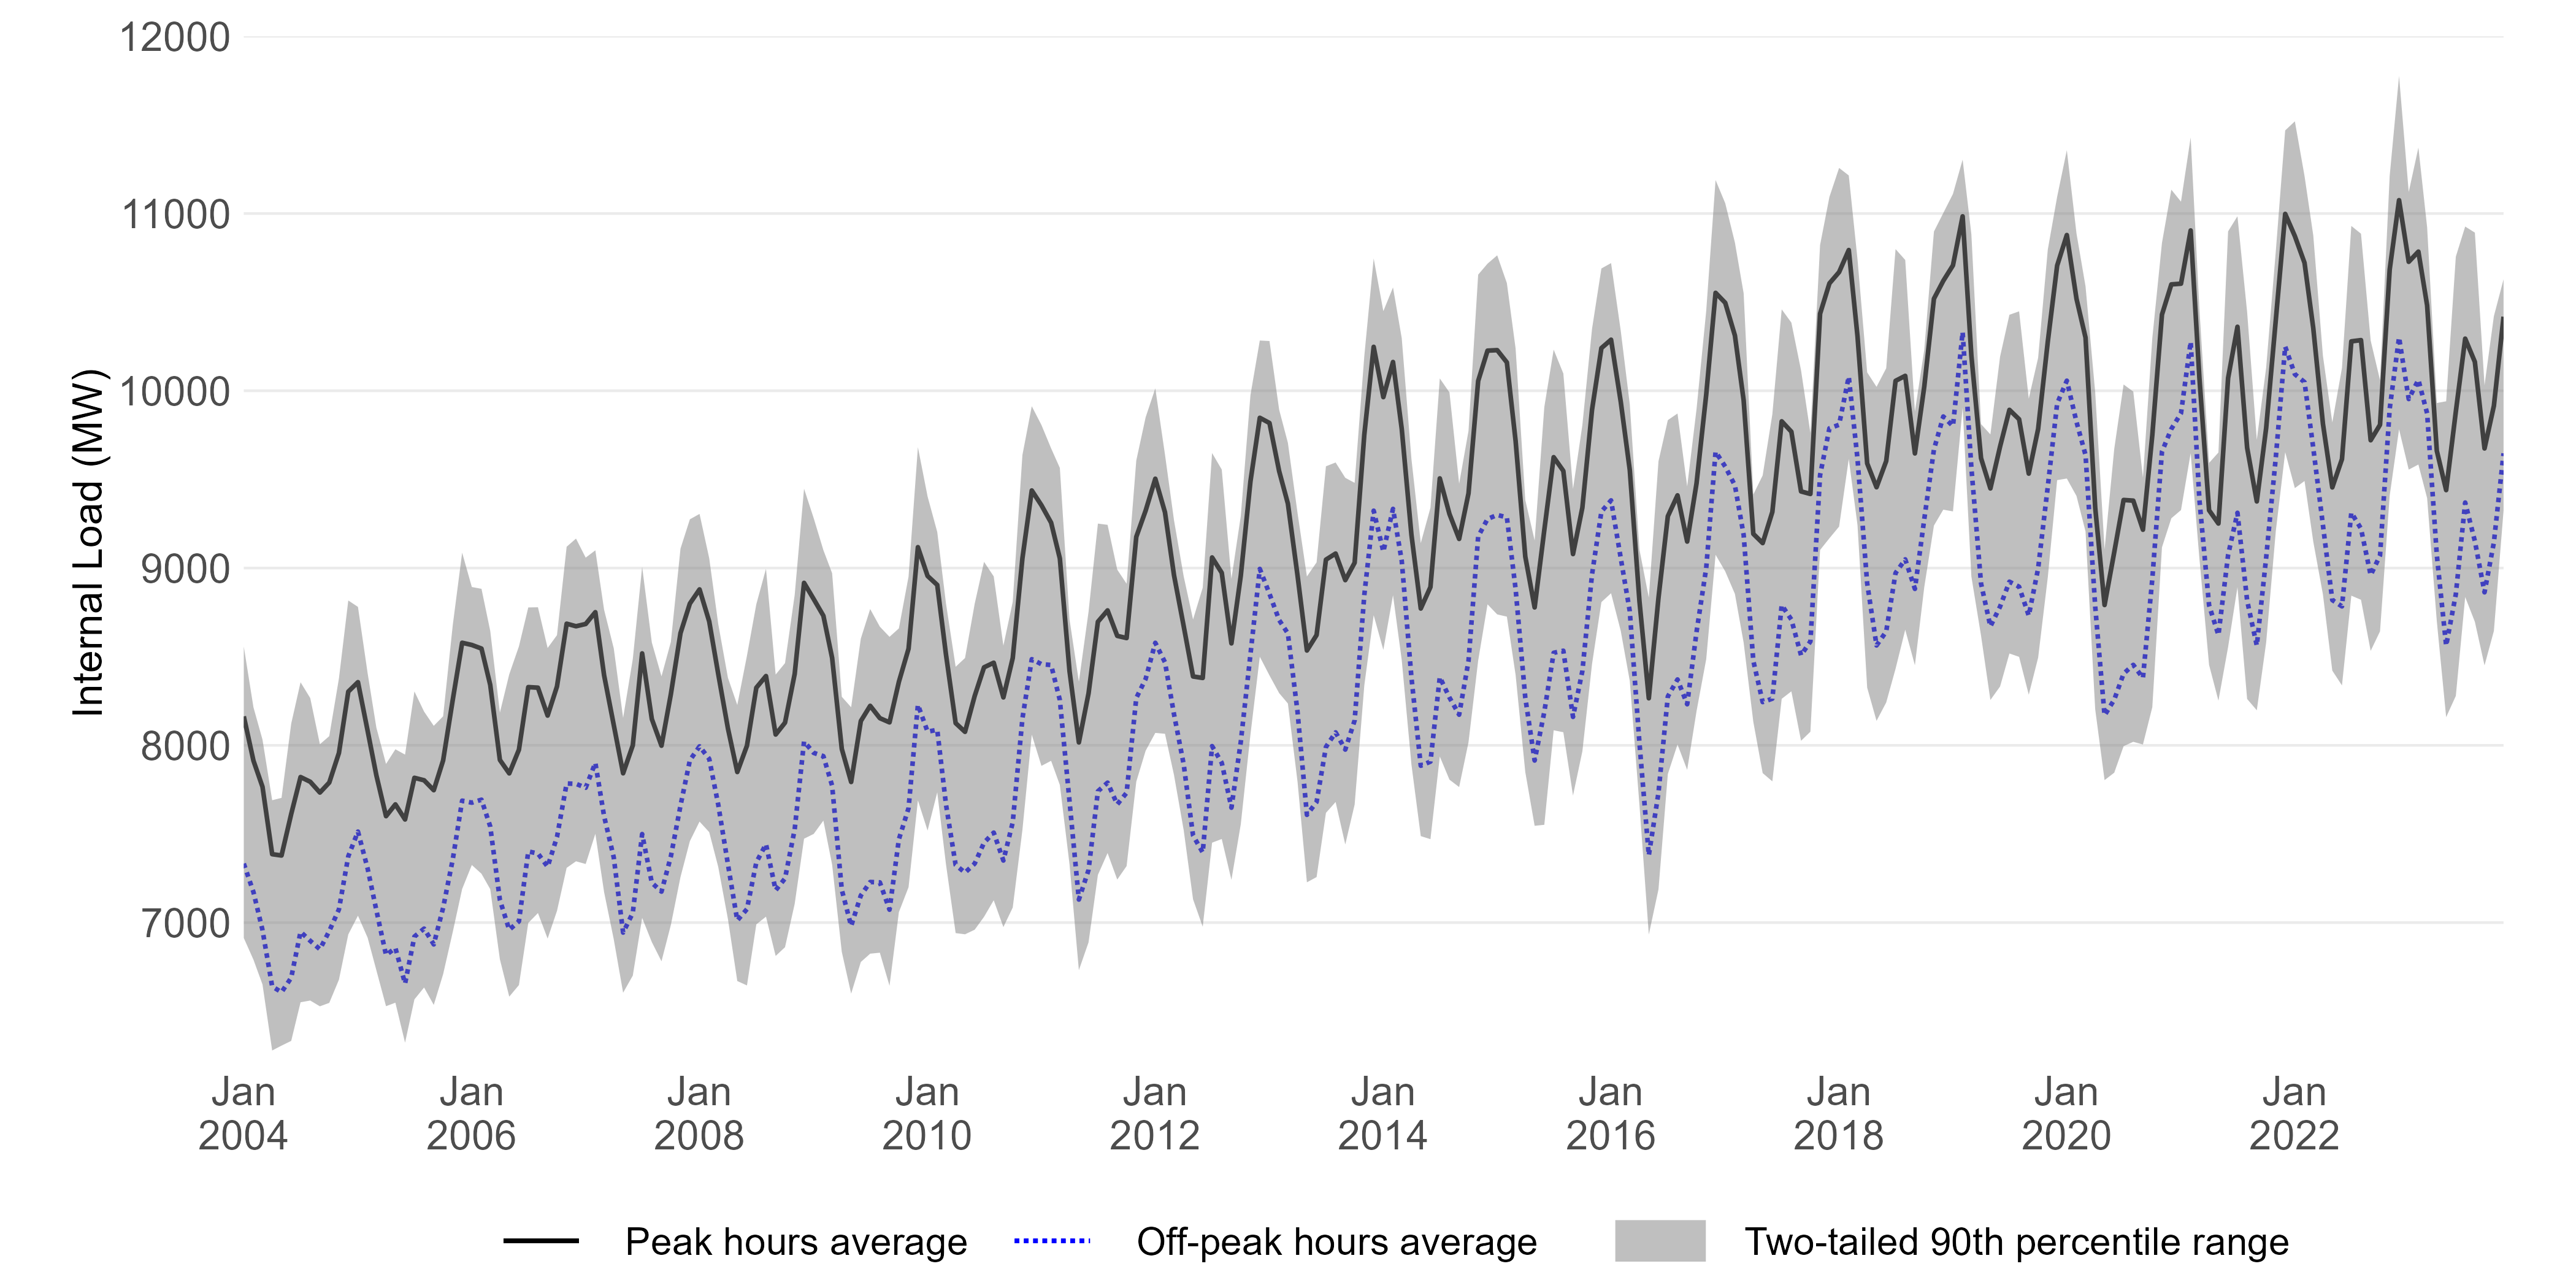
\includegraphics[width=6.5in]{../images/loads_clean.png}
\vspace{-0.75cm}	\caption{Alberta Internal Load. Source: Alberta Electric System Operator data.}
\label{fig:ab_load}
\end{figure}

Our sample period covers ten years with no major regulatory changes in the power market design. Alberta briefly considered an addition of a capacity market between 2016 and 2019, but this was never implemented. However, market conditions have varied over the sample period. There are three distinct periods during our sample - relatively high load growth and tight market conditions from 2009 through 2013, followed by sharply constrained growth and high reserve margins after 2014 through most of 2018, followed by a return to tighter market conditions after the spring of 2018. These conditions are reflected in peak and off-peak prices shown in Figure \ref{fig:ab_prices}. Some of these market changes coincide with policy changes of interest in our paper, in particular the changes to the \emph{SGER} introduced in June of 2015 which took effect in January of 2016 and 2017 respectively and are coincidental with a period of over-supply. Similarly, the introduction of the \emph{CCIR} in 2018 occurred during a period of tightening reserve margins and lingering uncertainty over market structure. From 2018 through pre-COVID 2020, both GHG policy and the wholesale electricity market were tightening, and so we need to be careful to disentangle these impacts.

\begin{figure}[t]%%
	\centering \vspace{-.25cm} 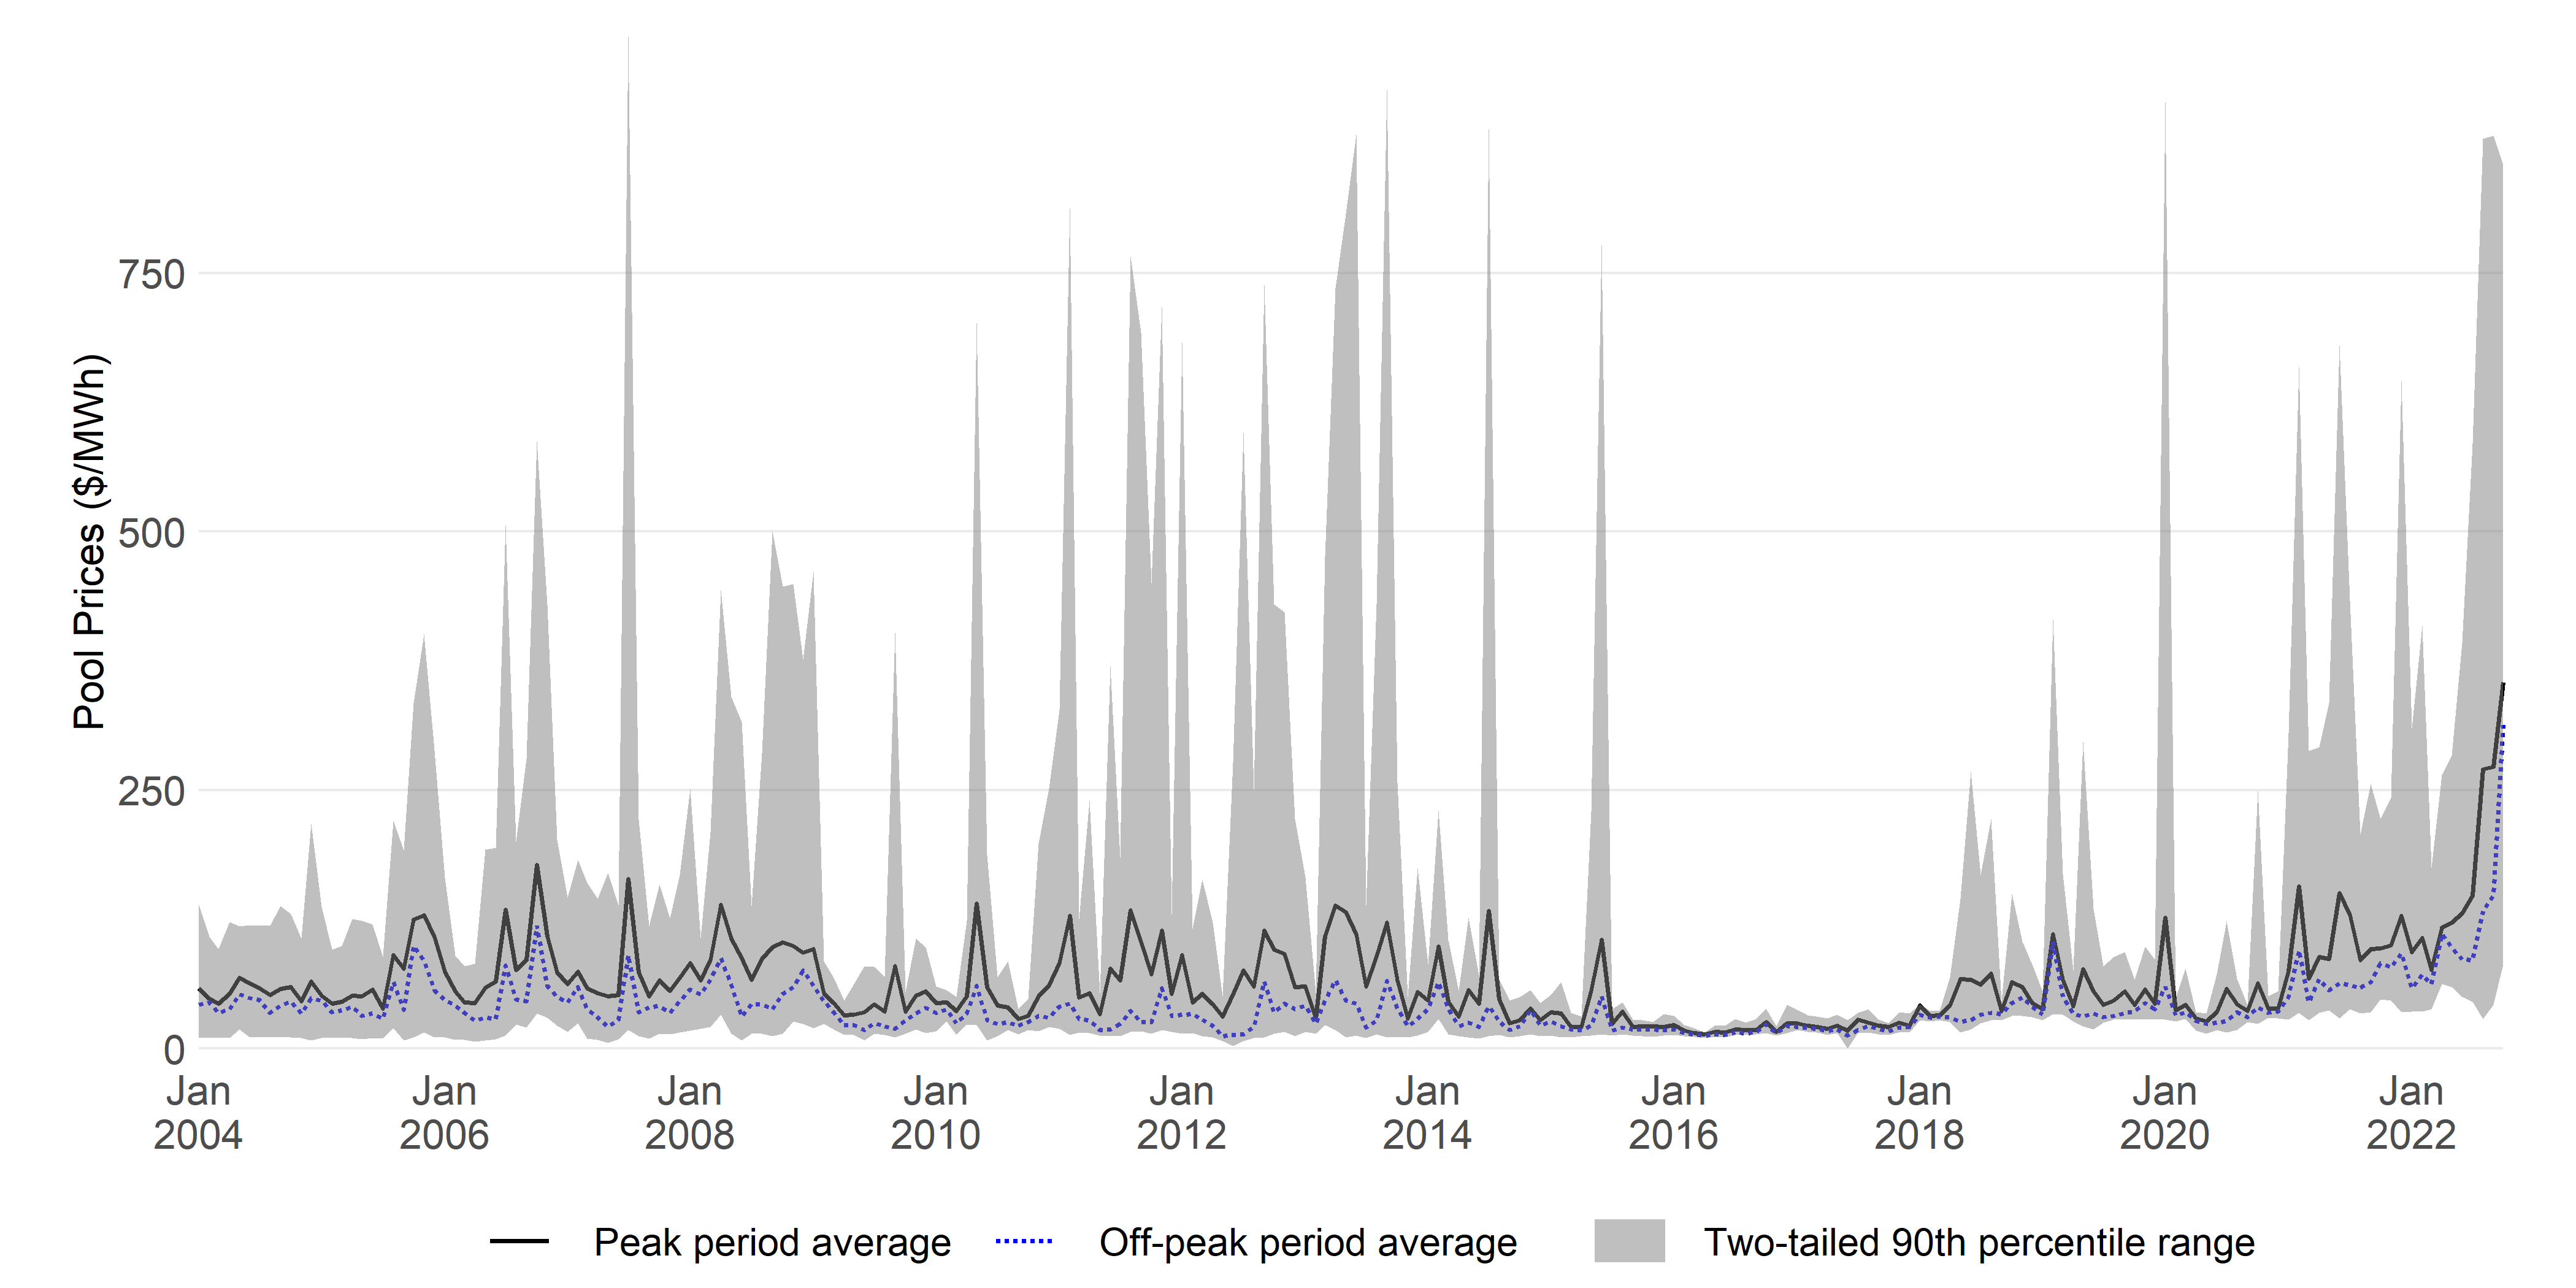
\includegraphics[width=6.5in]{../images/peak_prices.png}
\vspace{-0.75cm}	\caption{Wholesale power prices, peak and off-peak hours. Peak hours are 8am to 11pm other than on statutory holidays or Sundays. Source: AESO data, authors' graph.}
\label{fig:ab_prices}
\end{figure}

\begin{figure}[h]%%
	\centering \vspace{-.25cm} 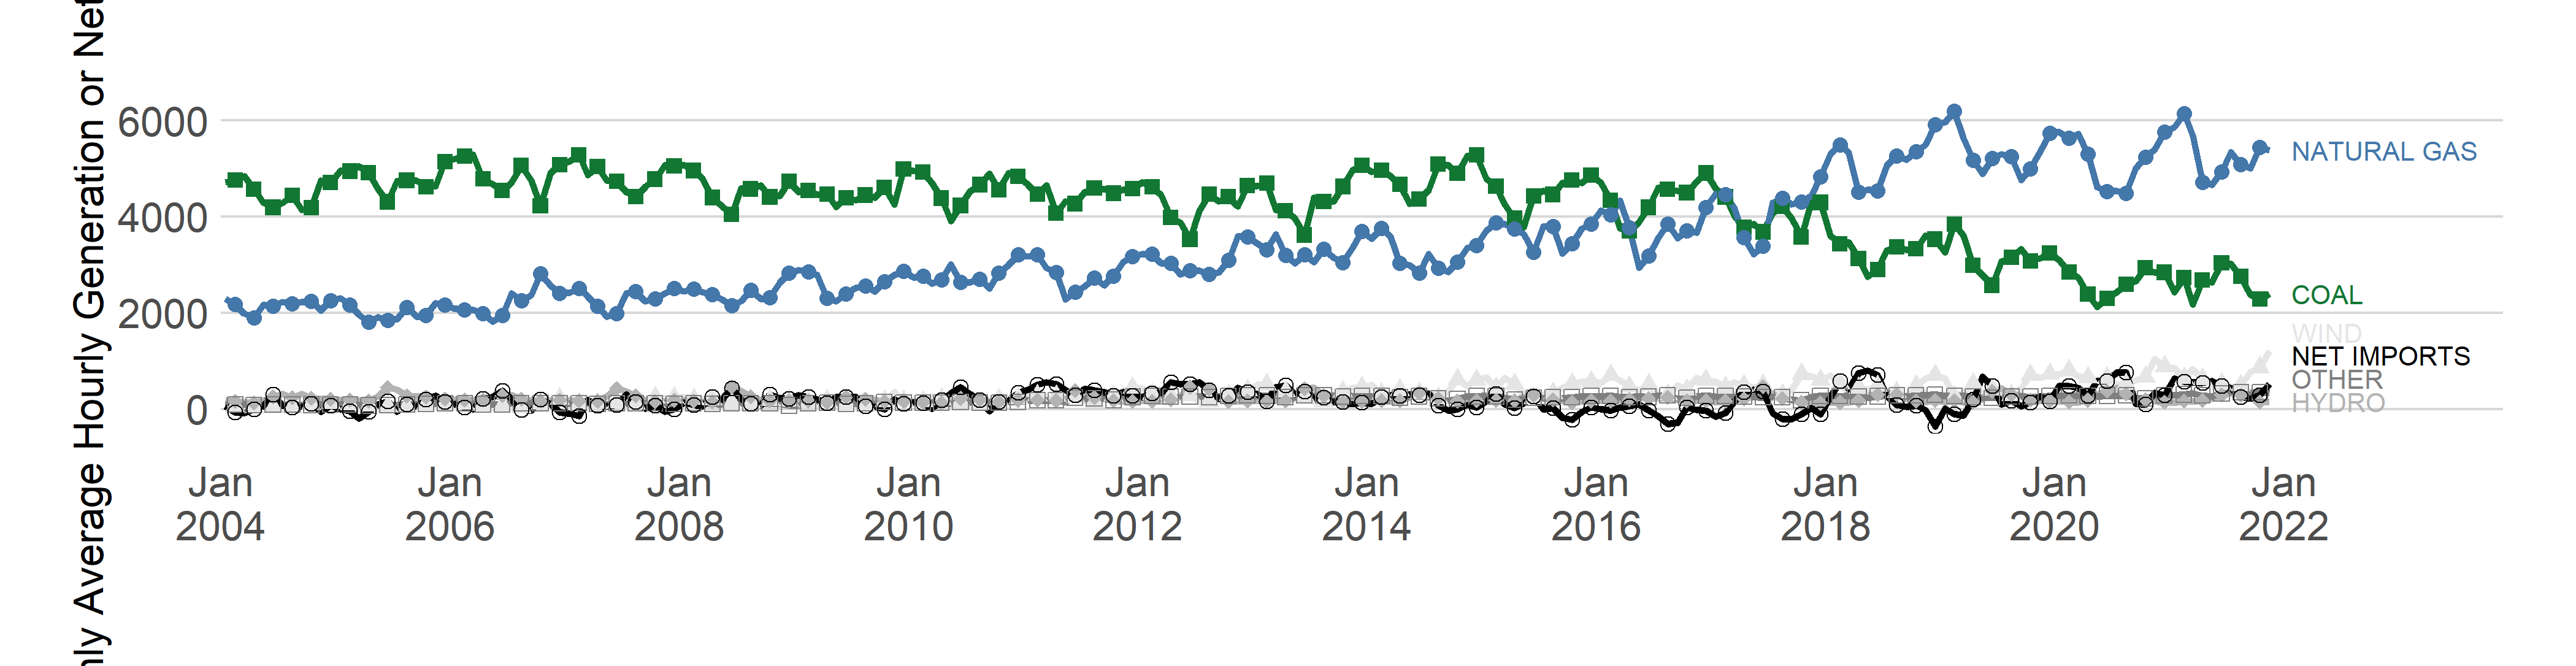
\includegraphics[width=6.5in]{../images/gen_fuel.png}
\vspace{-0.75cm}	\caption{Generation mix in Alberta.  Source: AESO data provided by NRGStream, authors' graph.}
\label{fig:gen_mix}
\end{figure}


The generation mix in Alberta's power market is dominated by fossil fuels although, as shown in Figure \ref{fig:gen_mix}, the dominant fossil fuel has changed from coal to natural gas. Within natural gas generation, the mix of plant types is also relevant to our study. During our sample period, a significant increase in generating capacity from combined cycle (NGCC) plants and combined heat and power (COGEN) facilities occurred. Combined heat and power plants tend to operate with high capacity factors but also tend to be price-takers in the market, with very little flexibility at the margin since the industrial processes with which they are associated rely on them for process heat.\footnote{As will be discussed below, net-to-grid power from COGEN facilities is primarily offered into the market at a \$0 offer and accepts market price, and so we see limited evidence of carbon price pass-through for most of the power offered by these facilities.} Combined-cycle plants, on the other hand, provided more flexible natural gas generation on the margin. Peaking capacity in the market during our sample period was largely met through ramping of coal and combined-cycle plants, as well as simple cycle (SCGT) natural gas turbines. Each of these would be exposed to carbon pricing, and so we expect to see pass through affect offers of power from these facilities into the market.

Consumption in Alberta is relatively stable on daily and annual bases due to the large industrial base. For example, in Figure \ref{fig:load_pattern}, we compare Alberta's hourly load pattern to ERCOT and MISO equivalents. In the left-hand panel, we see that there is less variability through the day in Alberta as industrial load dominates cycles in residential and commercial load. Seasonal patterns are also both less pronounced and exhibit a winter peak, compared to the summer-peaking ERCOT and MISO systems.

\begin{figure}[!h]%%
	\centering \vspace{-.25cm} \includegraphics[width=6.5in]{../images/load_compare.png}
\vspace{-0.75cm}	\caption{Monthly and hourly load patterns in Alberta compared to ERCOT and MISO.}
\label{fig:load_pattern}
\end{figure}

Alberta's wholesale market is such that different generators will derive different levels of average revenue from the sale of their power. Those that dispatch only in high-price times will have higher revenues on average than plants without dispatch control, or plants which run most hours of the day. Since prices have varied substantially over time, as shown above in Figure \ref{fig:ab_prices}, captured average prices at the plant level have varied as well, as shown in Figure \ref{fig:capture_prices}. We can see evidence here of how plants of different types offer their power into the market: hydro and combined- and simple-cycle gas turbines follow prices, and dispatch more often in higher-priced hours, just as imports tend to occur when prices are higher. Prices tend to be negatively correlated with wind generation, and so captured prices for wind power facilities are lower than other forms of generation. Exports tend to be scheduled when prices are expected to be low, which is reflected in the graph. Solar, a relatively new entrant in the Alberta market, has captured higher prices than other variable renewable sources since its generation pattern coincides with daily and seasonal peak prices, although we would expect this to change as \emph{duck curve} effects take hold over time.

\begin{figure}[t]%%
	\centering \vspace{-.25cm} 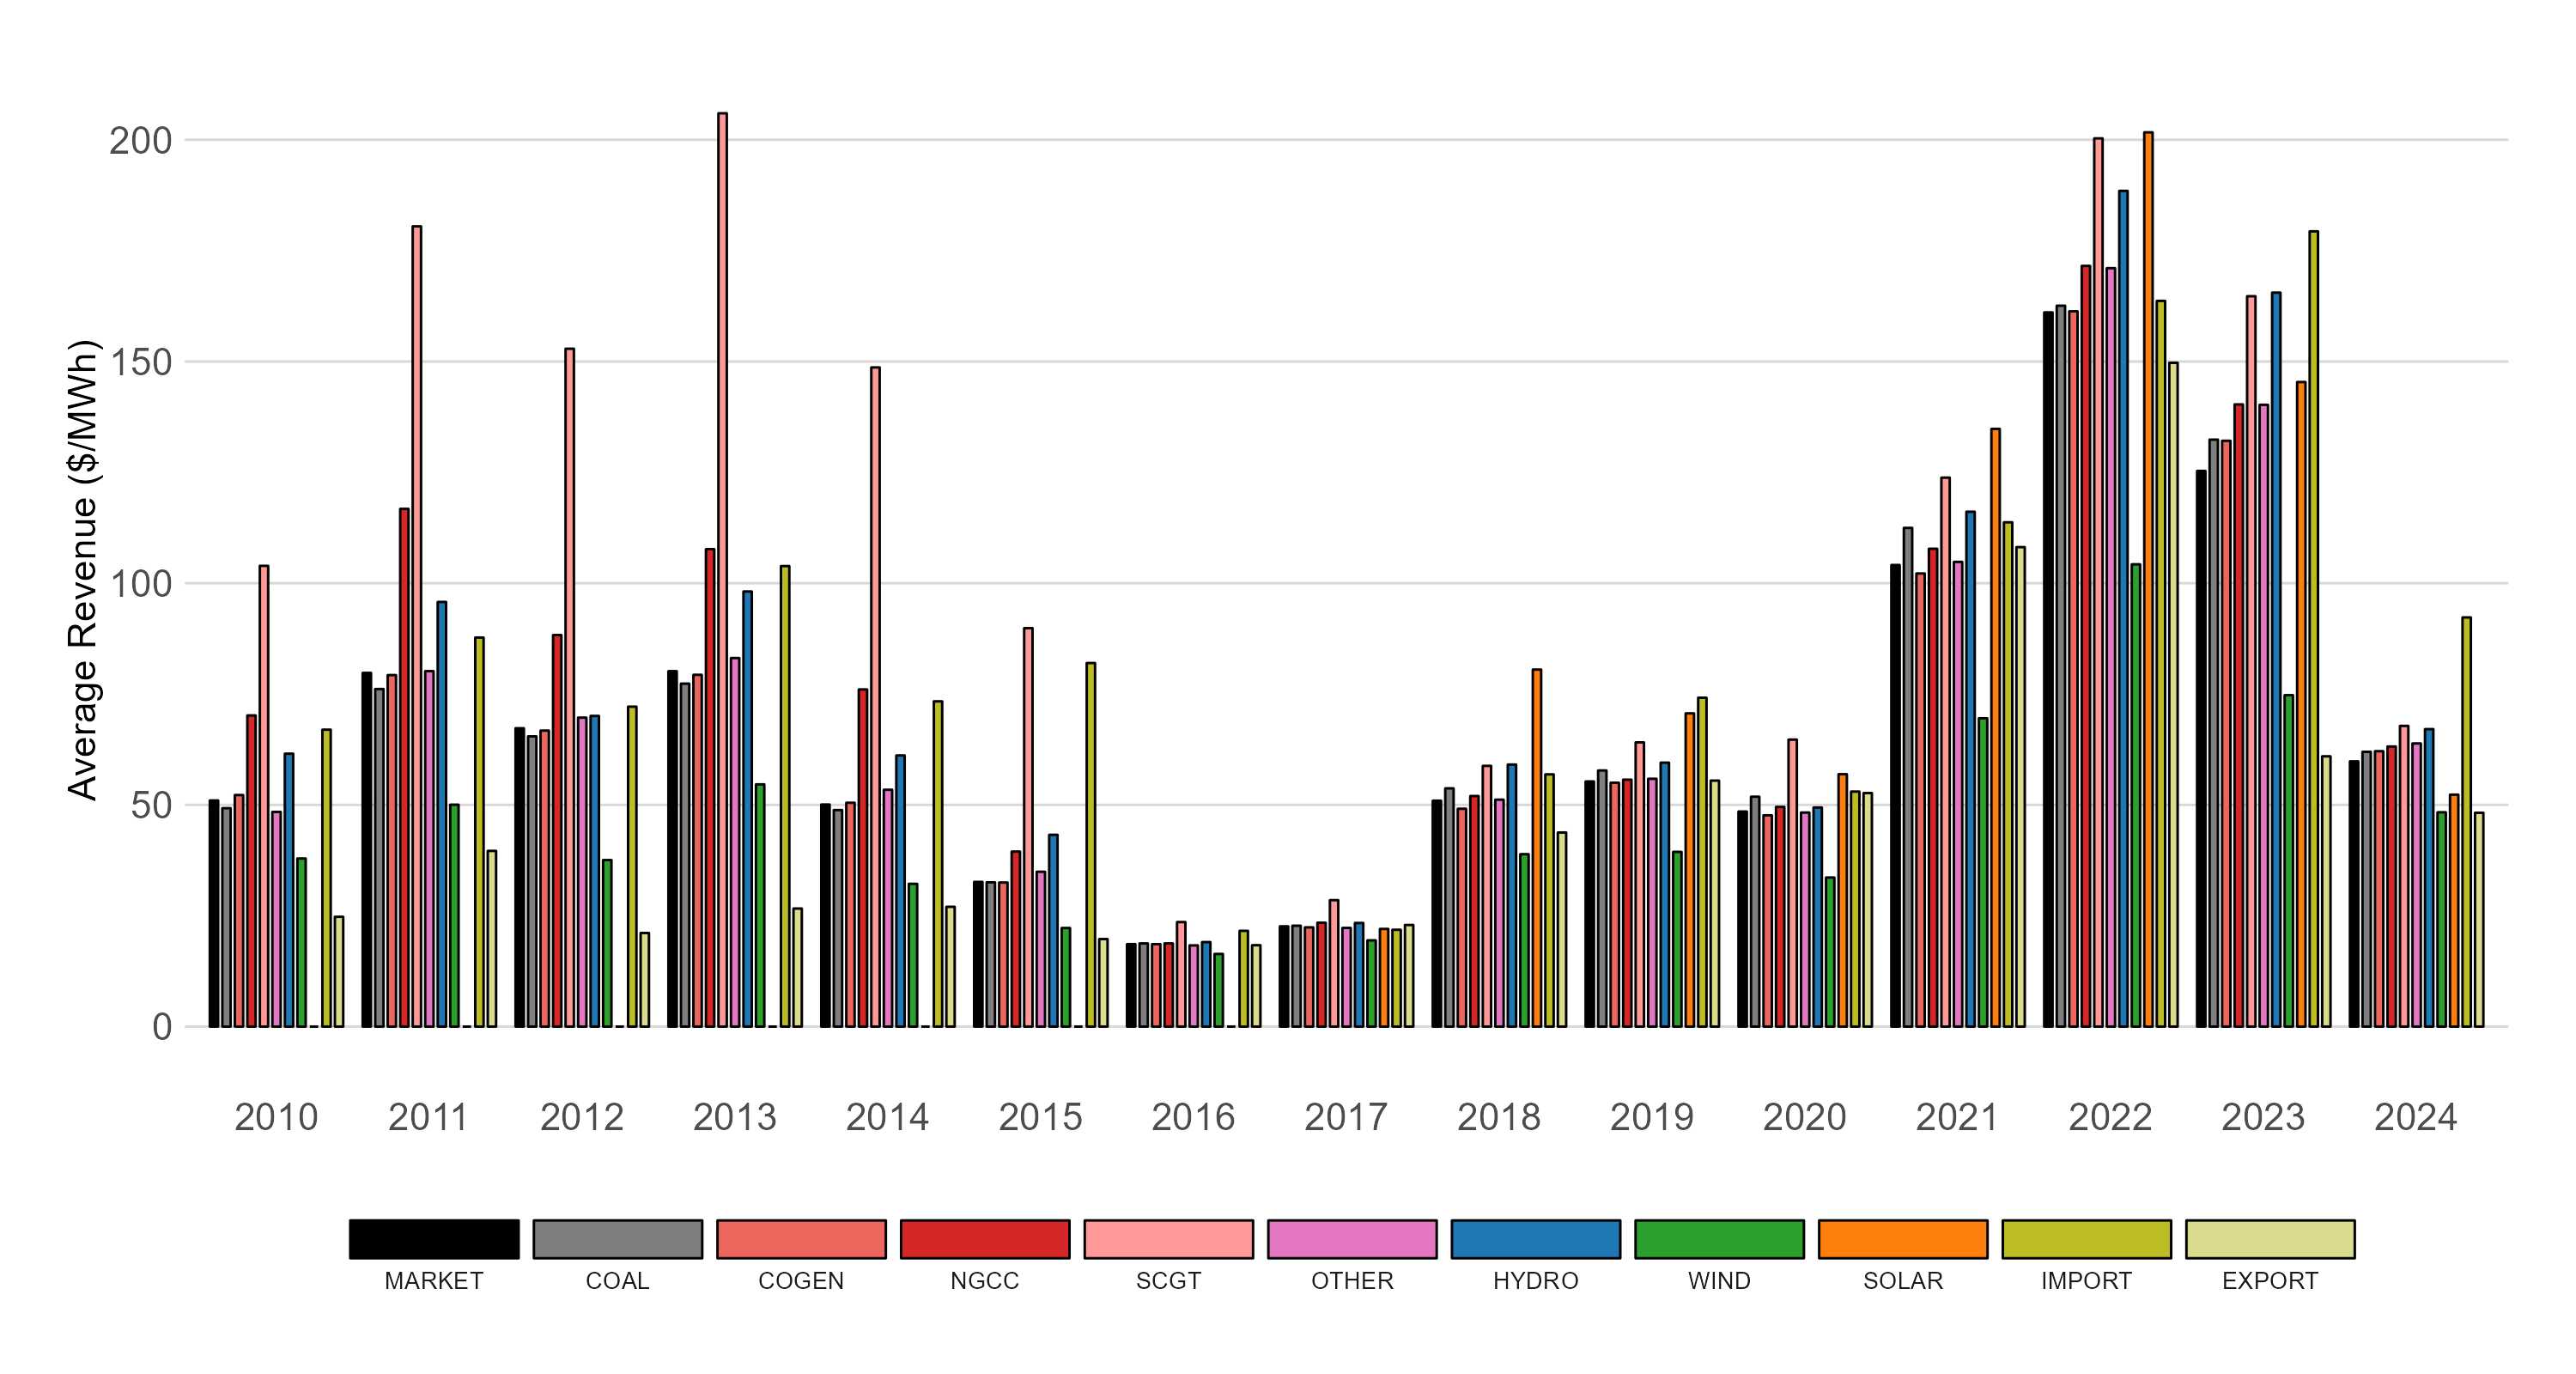
\includegraphics[width=6.5in]{../images/price_capture.png}
\vspace{-0.75cm}	\caption{Annual average revenue by plant type. Source: AESO generation data provided by NRGStream, authors' graph.}
\label{fig:capture_prices}
\end{figure}

Finally, Alberta's market is highly concentrated, with a market structure that has evolved in ways relevant to our analysis during the relevant time period. When the market was restructured in 2000, a system of power purchase arrangements (PPAs) were used as an alternative to divestment. Large coal-fired plants owned by legacy generators were covered by these PPAs which approximated the conditions for plant owners which had been present under regulation, while auctioning off the rights to offer control over these facilities to other entities. PPAs not sold in the auction were held by an entity known as the Balancing Pool. The PPAs included a cumbersomely-worded change-of-law clause which was interpreted to imply a option for PPA owners to exit these arrangements should they become unprofitable or ``more unprofitable" due to a change in law, and several PPA owners exercised this right during our period of study, specifically in response to the changes in carbon pricing policy announced in June of 2015. As detailed in Leach and Tombe (2016)

As shown in Table \ref{tab:PPA}, a substantial amount of Alberta's generating capacity (5066 MW) was offered into the market under these PPAs during our study period, and the majority (3866 MW) of that was transferred back to the Balancing Pool in early 2016. The reason for this change was the erosion in the profitability of the PPAs contributed to by changes in carbon pricing. But, the coincidence of changes in offer control with changes in carbon pricing in early 2016 have the potential to confound our inference.

\begin{table}
\begin{tabular}{lccccc}
  \hline\\[-1.75ex]
Facility&Plant&Unit& Capacity& End of& Returned to\\
&Owner&         ID   &  (MW) &  PPA Term &Balancing\\
&&                 &    &      & Pool\\[+0.5ex]
\hline \\[-1.5ex]
Battle River& ATCO& BR3 &147& Dec-31-2013&NA\\
&&BR4 &147& Dec-31-2013&NA\\
&&BR5 &368& Dec-31-2020&Jan-1-2016\\[+0.75ex]
Genesee &Capital Power &GN1 &381 &Dec-31-2020&NA\\
&&GN2 &381 &Dec-31-2020&NA\\[+0.75ex]
HR Milner &ATCO& HRM& 144& Jan-01-2013&NA\\[+0.75ex]
Keephills& TransAlta & KH1 &383& Dec-31-2020&May-5-2016\\
&&KH2& 383& Dec-31-2020&May-5-2016\\[+0.75ex]
Sheerness &ATCO (50\%) & SH1& 378& Dec-31-2020&Mar-7-2016\\
&TransAlta (50\%)&SH2& 378& Dec-31-20200&Mar-7-2016\\[+0.75ex]
Sundance A &TransAlta&  SD1 &280& Dec-31-2020&Mar-7-2016\\
&&SD2 &280& Dec-31-20200&Mar-7-2016\\[+0.75ex]
Sundance B &TransAlta & SD3& 353& Dec-31-2020&Mar-7-2016\\
&&SD4 &353 &Dec-31-20200&Mar-7-2016\\[+0.75ex]
Sundance C &TransAlta& SD5& 353& Dec-31-2020&Mar-24-2016\\
&&SD6& 357& Dec-31-20200&Mar-7-2016\\[+0.75ex]
  \hline
\end{tabular}
\caption{Alberta coal-fired plant Power Purchase Arrangement (PPA) expiry dates and dates of return to the Balancing Pool}\label{tab:PPA}
\end{table}







\begin{figure}[t]
    \centering
    \begin{minipage}{\textwidth}
        \centering
        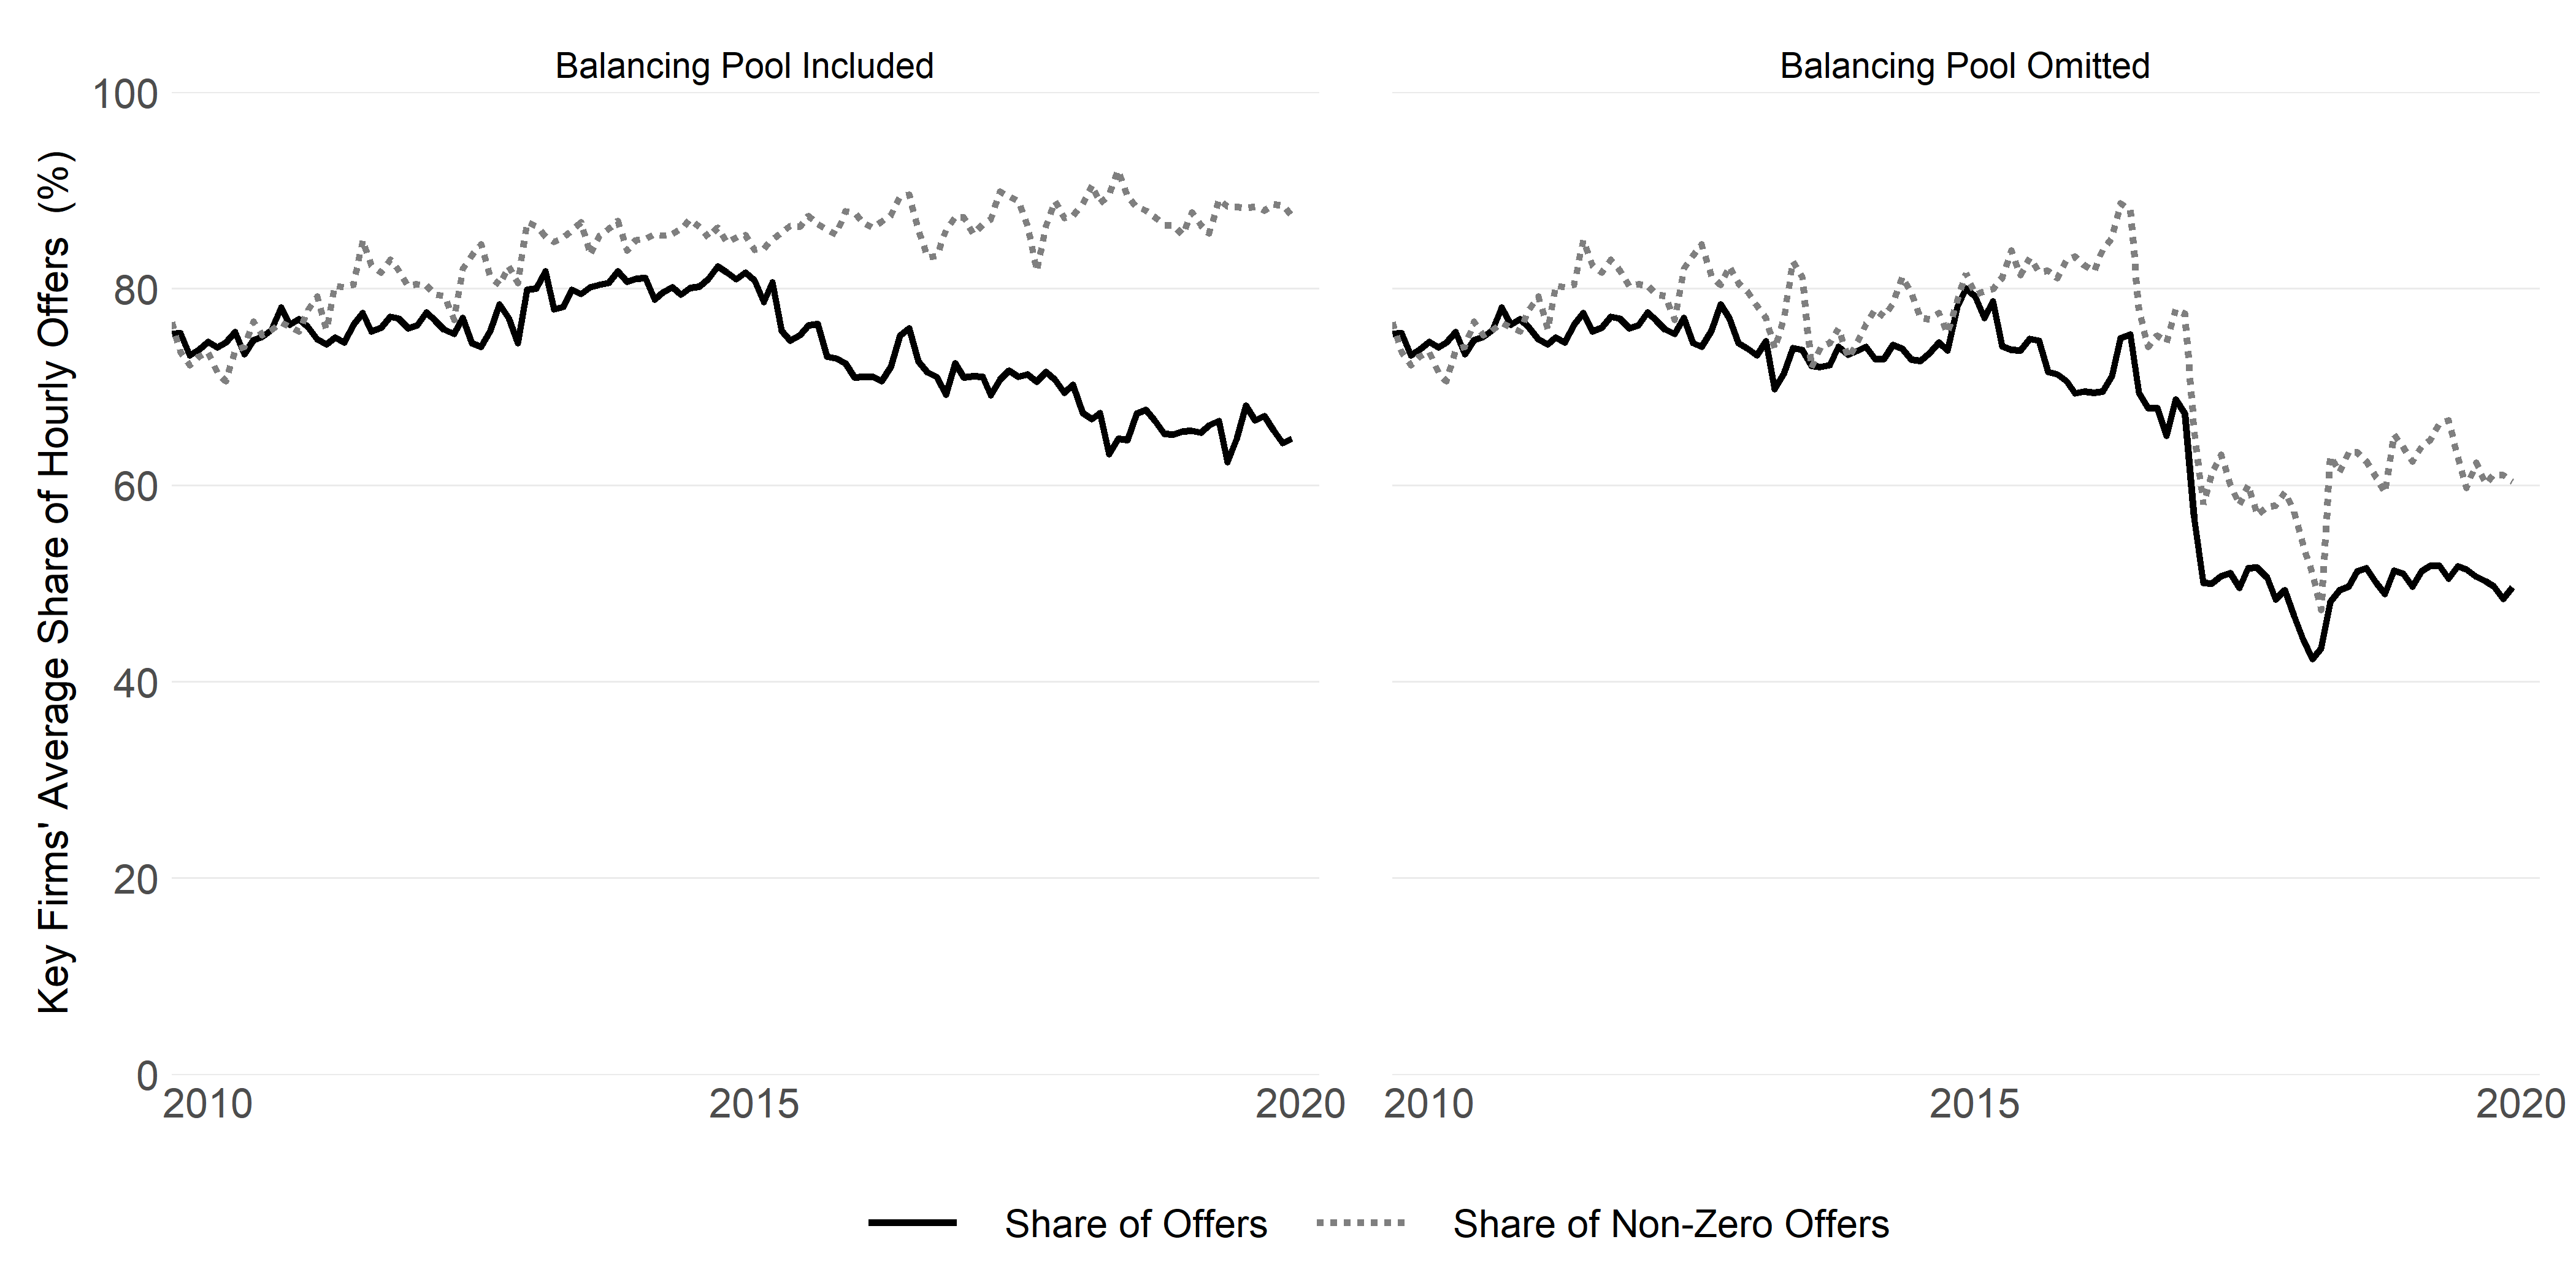
\includegraphics[width=.9\textwidth]{../images/mkt_power.png}
        \caption{Share of offer control and share of non-zero offers from key firms including and not including the Balancing Pool government-owned corporation. Key firms include TransAlta, Capital Power, ENMAX, ATCO, Heartland Generation, and TransCanada, with the addition of the Balancing Pool in the left-hand panel.}
    \label{fig:synth_illust}
        %\caption{$dt=0.1$}
        %\label{fig:prob1_6_2}
    \end{minipage}%
\end{figure}






\section{The Impact of Carbon Pricing Policy Changes}

Alberta's three carbon pricing regimes each affected generating facilities in two ways. First, each of three (\emph{SGER}, \emph{CCIR}, and \emph{TIER}) regimes imposes a price on emissions. Second, each regime allocates emissions credits based on output or deemed avoided emissions. The net effect of these policies creates variation within and across facilities and facility types and over time.  Consider, for example, Figure \ref{fig:sector_compliance_cost} which shows the mean value and range of annual compliance costs for larger generators in Alberta's fleet over the sample period.\footnote{Plants were only included in the sample for this figure if we had facility-specific compliance cost data. For our estimation results, we impute compliance costs for a wider set of facilities using emissions intensities from the compliance cost data.}

\begin{figure}[t]%%
	\centering \vspace{-.25cm} \includegraphics[width=6.5in]{../../SGER/sector_compliance_cost.png}
\vspace{-0.75cm}	\caption{Generation-weighted annual average compliance cost (dashed black lines) and individual plant realizations (lighter grey lines) by plant type (\$/MWh), combined with the price charged on excess net annual emissions (black lines) under Alberta's carbon pricing programs (\$/tonne). Coal plants and natural gas combined-cycle (NGCC) and simple-cycle (SCGT) plants with more than 20MW installed capacity are shown. Source: Alberta Environment compliance cost data combined with AESO generation data provided by NRGStream.}
\label{fig:sector_compliance_cost}
\end{figure}

As Figure \ref{fig:sector_compliance_cost} shows, changes in facility compliance costs were not all coincident with increased marginal carbon prices. In fact, the compliance cost changes are mostly determined  by the changes in output-based allocations which occurred subsequent to the adoption of the \emph{CCIR} in 2018 rather than the initial increase carbon prices from \$15 to \$30 per tonne \coe in 2016 and 2017. The largest cost increases were experienced by coal-fired power plants and some simple-cycle generators, while limited effects were felt by combined heat and power plants (not shown). Compliance costs for natural gas combined-cycle plants dropped between 2017 and 2019 as a result of a change in the formula by which output-based allocations were calculated. These changes in compliance costs, across and within generators, provide the variation through which we identify pass-through to power offers.

\section{Estimation Strategy}
The focus of our estimation strategy is to identify the magnitude of the vertical shift in the electricity supply curves for the market as a whole or aggregated by generator fuel or controlling entity in response to changes in carbon pricing policies.

There are multiple factors which confound our ability to draw inference from the merit order data. The first is that plants of the same type (e.g. coal or combined-cycle natural gas plants) may be of different sizes (e.g. a 350MW plant vs a 200MW plant) while facing similar optimization constraints, and they may be jointly dispatched by the same operator. In particular for coal plants, plant-level minimum-must-run constraints imply that facilities will always offer some portion of their generation into the market at a \$0/MWh price, effectively acting as price takers for an endogenously-determined share of their generation. Given that shutting down in any given hour would imply multiple hours out of the market, the true marginal opportunity cost of this power is negative. They may offer marginal blocks of power, for capacity above their minimum-must-run level, at higher prices. However, given that plants are of different sizes, and blocks are endogenously determined, it's challenging to identify a change in offers looking only at block offers. The second issue is that the strategy space for each facility is very large, given that they may decide both on the break-points for each of up to 7 blocks of power, and then decide on a price for the first block and an adder for each subsequent block offered into the market. For each hour, then, the optimization problem consists of 12 choice variables and we have data on these choices for almost 20 million facility-hour-block pairs. Finally, since multiple plants may be controlled by a single entity, the observed data are the product of a complex portfolio optimization problem and the offers of any individual plant may not reveal an overall portfolio-level attempt to pass through the costs of carbon prices to wholesale prices. We avoid these problems by constructing synthetic offer curves either by plant-type and by controlling entity, or for the market as a whole, thus estimating the impact of policy changes on the supply behaviour of the aggregate fleet rather than on any individual plant. We then use the synthetic merit order data we construct to examine how power has been offered into the system over time as climate policies have varied.

To understand our approach, consider the traditional textbook treatment of carbon pricing or output-based allocations, which would imply a vertical shift in the supply curve corresponding to the increased marginal cost or the carbon tax, with a negative shift in the case of output-based allocations which reduce net costs of generation. The horizontal summation of all of the individual firm supply curves should imply that, all else equal, the vertical shift in the market supply curve at any point is equal to the marginal cost impact of the carbon policy on the firm which would supply that particular marginal unit of power. We have data on these horizontally-summed supply curves and, by sampling specific points on the supply curve over time, we identify the magnitude of pass-through.

\begin{figure}[t]
    \centering
    \begin{minipage}{\textwidth}
        \centering
        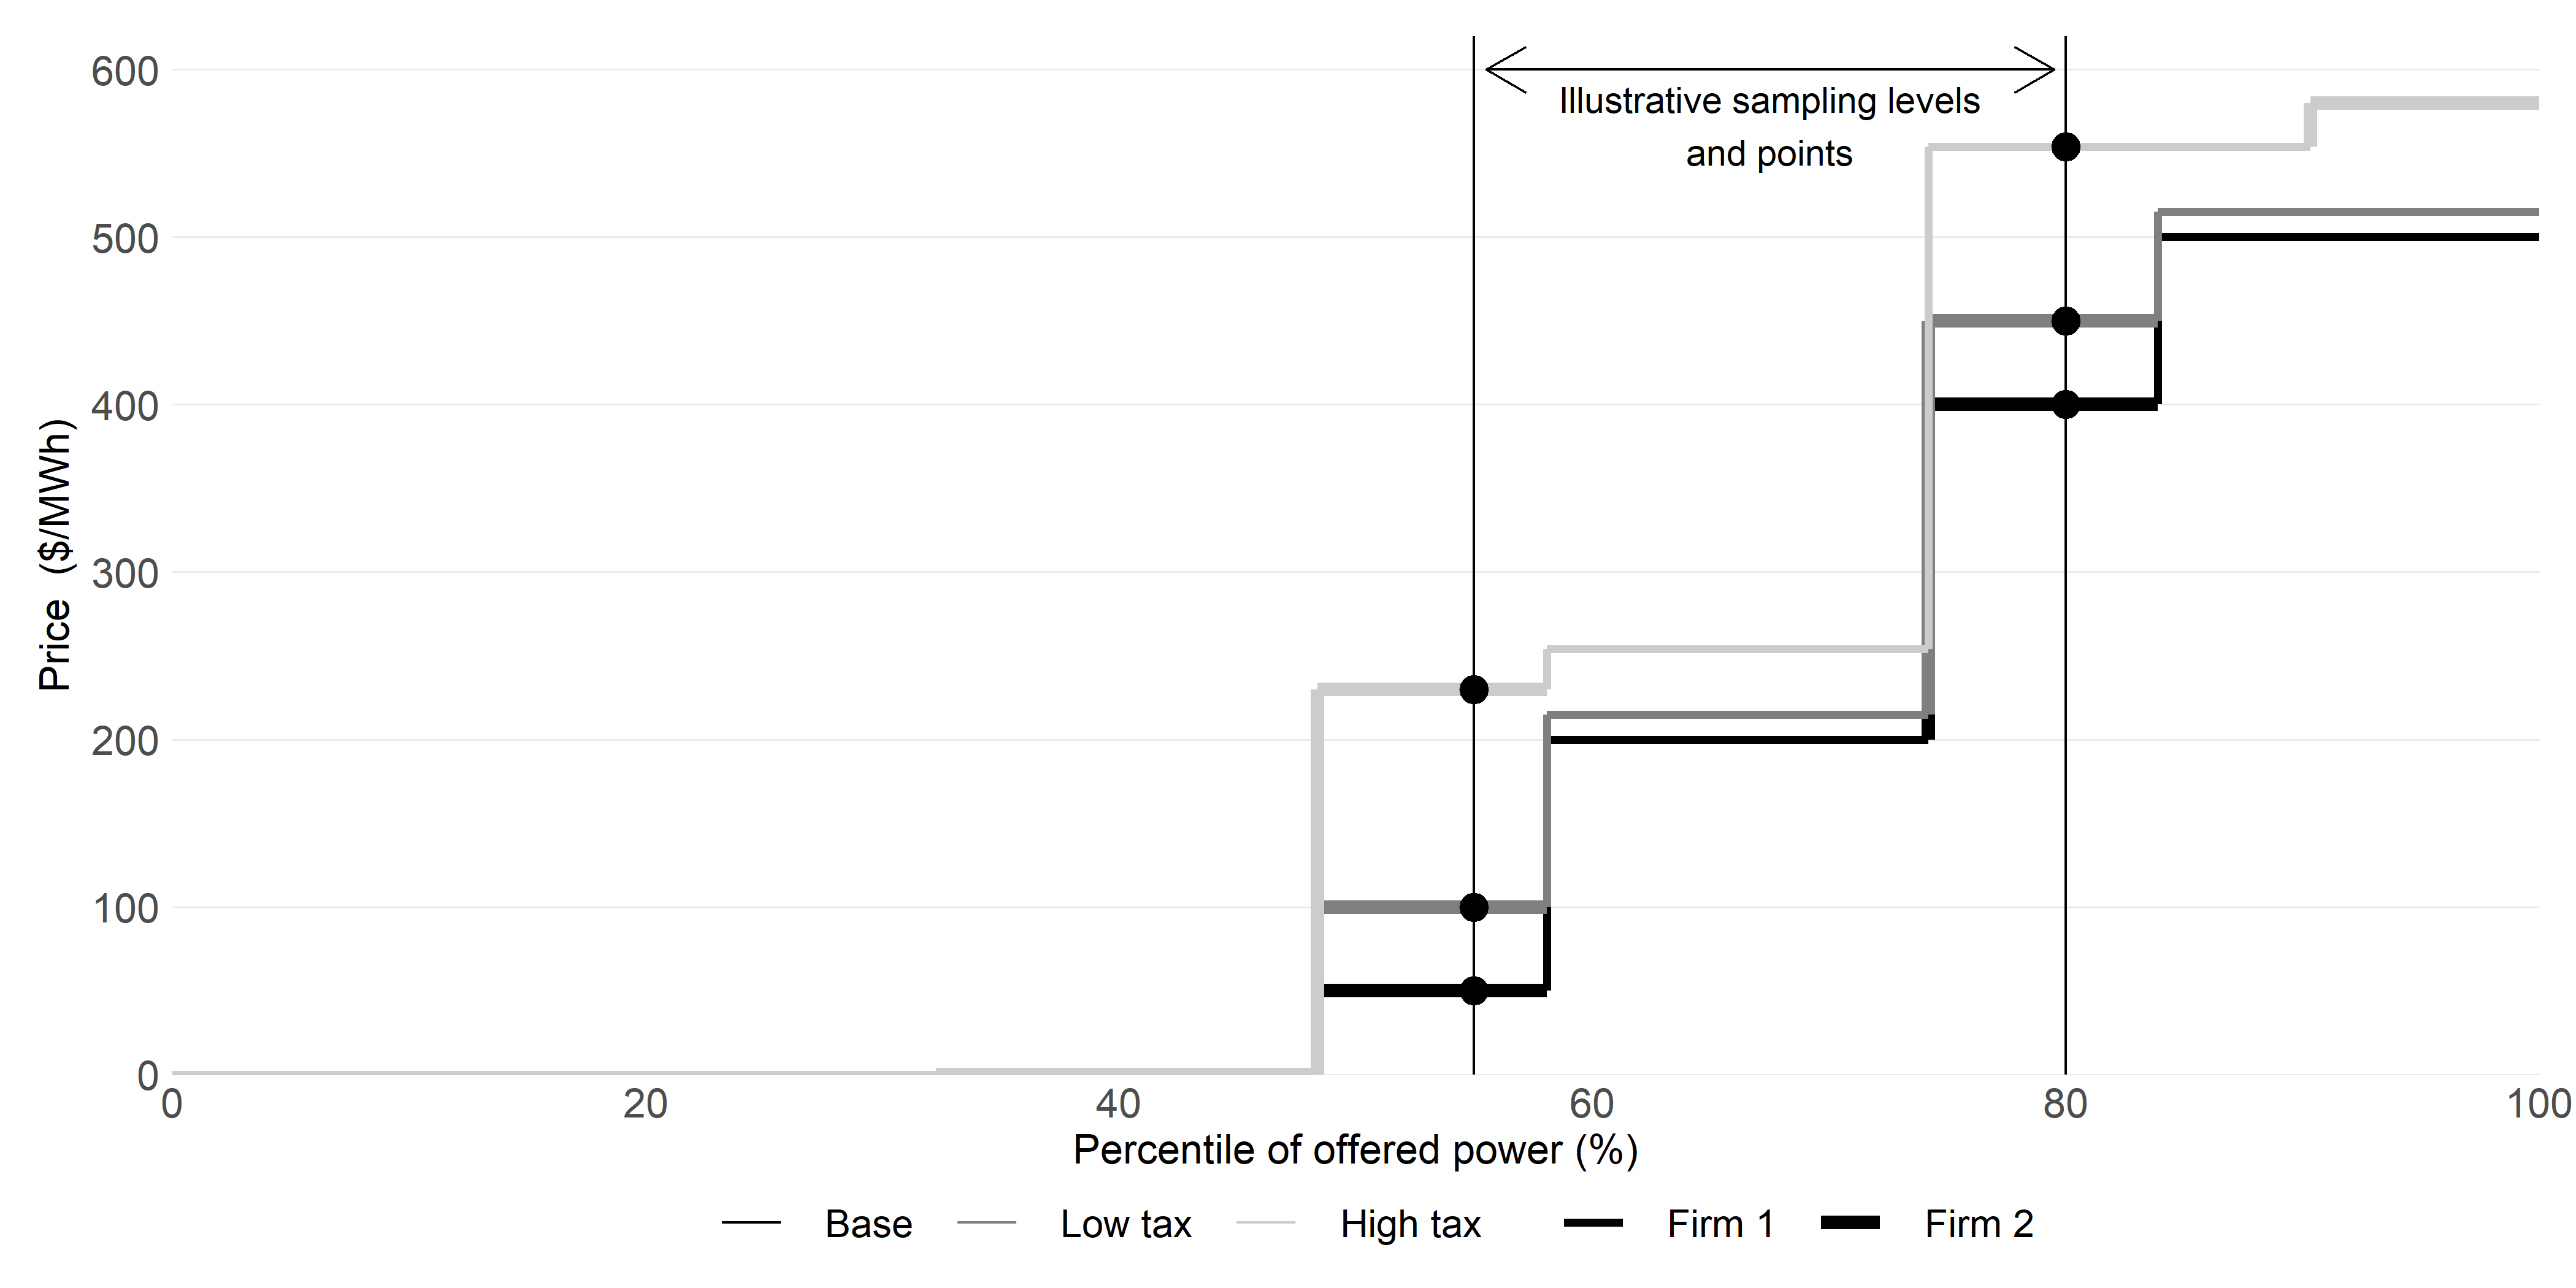
\includegraphics[width=.9\textwidth]{../images/sampling.png}
        \caption{Illustration of two firms' (thicker and thinner lines) offers of power in no-, high-, and low-carbon-tax scenarios, with lighter grey lines indicating a higher carbon price.}
    \label{fig:synth_illust}
        %\caption{$dt=0.1$}
        %\label{fig:prob1_6_2}
    \end{minipage}%
\end{figure}

To measure this effect, we look at hourly merit orders and sample at multiple percentile points, using more sampling points at the upper end of the merit order. The variation in carbon pricing over time, as well as variation in which firms are participating in the market at different times allows us to develop a sample of offer values at each of our chosen percentile nodes over our entire sample. For each sampled point, we identify facility and market conditions, as well as carbon policy compliance costs, which we use to explain changes in the level offer levels over time. Consider the illustrative example in Figure \ref{fig:synth_illust} which shows shifts in a hypothetical two-firm supply curve in response to increasing carbon prices. At the 55th percentile, the first sampling point shown, the vertical shift is driven entirely by pass-through from Firm 2 of their marginal carbon costs over-and-above the base case. At the 80th percentile, the second sampling point shown, the increase under the low-tax scenario is caused by the pass-through from Firm 2, but in the higher carbon tax scenario, the vertical shift is a smaller than would be the case for a pure pass-through by Firm 2 since there is also a shift in the ordering of offered blocks such that a different firm is providing the 80th percentile supply into the market with the high carbon tax.

To show what this implies for actual data, consider Figure \ref{fig:synth_merit}. In the left-hand panel, we show the merit order for one hour for all of the coal-powered facilities in the province, with offers from multi-unit facilities combined for ease of visualization. We see facilities bidding some of their power at \$0, ensuring they are in the market, with marginal generation blocks offered at increasing marginal prices. In this particular hour, the price was such that most of the offered coal generation was dispatched, with only blocks offered above the \$802/MWh market clearing price not being dispatched. In the right hand panel, we show our sampling of the merit order which summarizes all of the coal power offered into the market in a given hour using the 15 points shown in the Figure, which correspond to the value of the merit order at prescribed percentiles of the total offered power in that hour.\footnote{We store the 10th through 40th percentiles in 10\% intervals and the 50th percentile and above in 5\% intervals to better capture the curvature of the merit order.} Summarizing the data this way reduces our stored information by a factor of three, but more importantly it allows us to answer the relevant question in our study - by how much did the supply curve shift in response to changes in the value of carbon pricing costs and output-based allocation revenue - by looking at changes in the value of our sampling points across the portfolio of offered power. Or, visually, we want to ask how, on average, each of the points in the right-hand panel of Figure \ref{fig:synth_merit} change when carbon prices are increased or when output-based allocations of emissions credits change. For each of these sampled points, we include relevant facility- and market-level data as well as carbon tax compliance costs for that facility on that date.

\begin{figure}[tb]
    \centering
    \begin{minipage}{.5\textwidth}
        \centering
        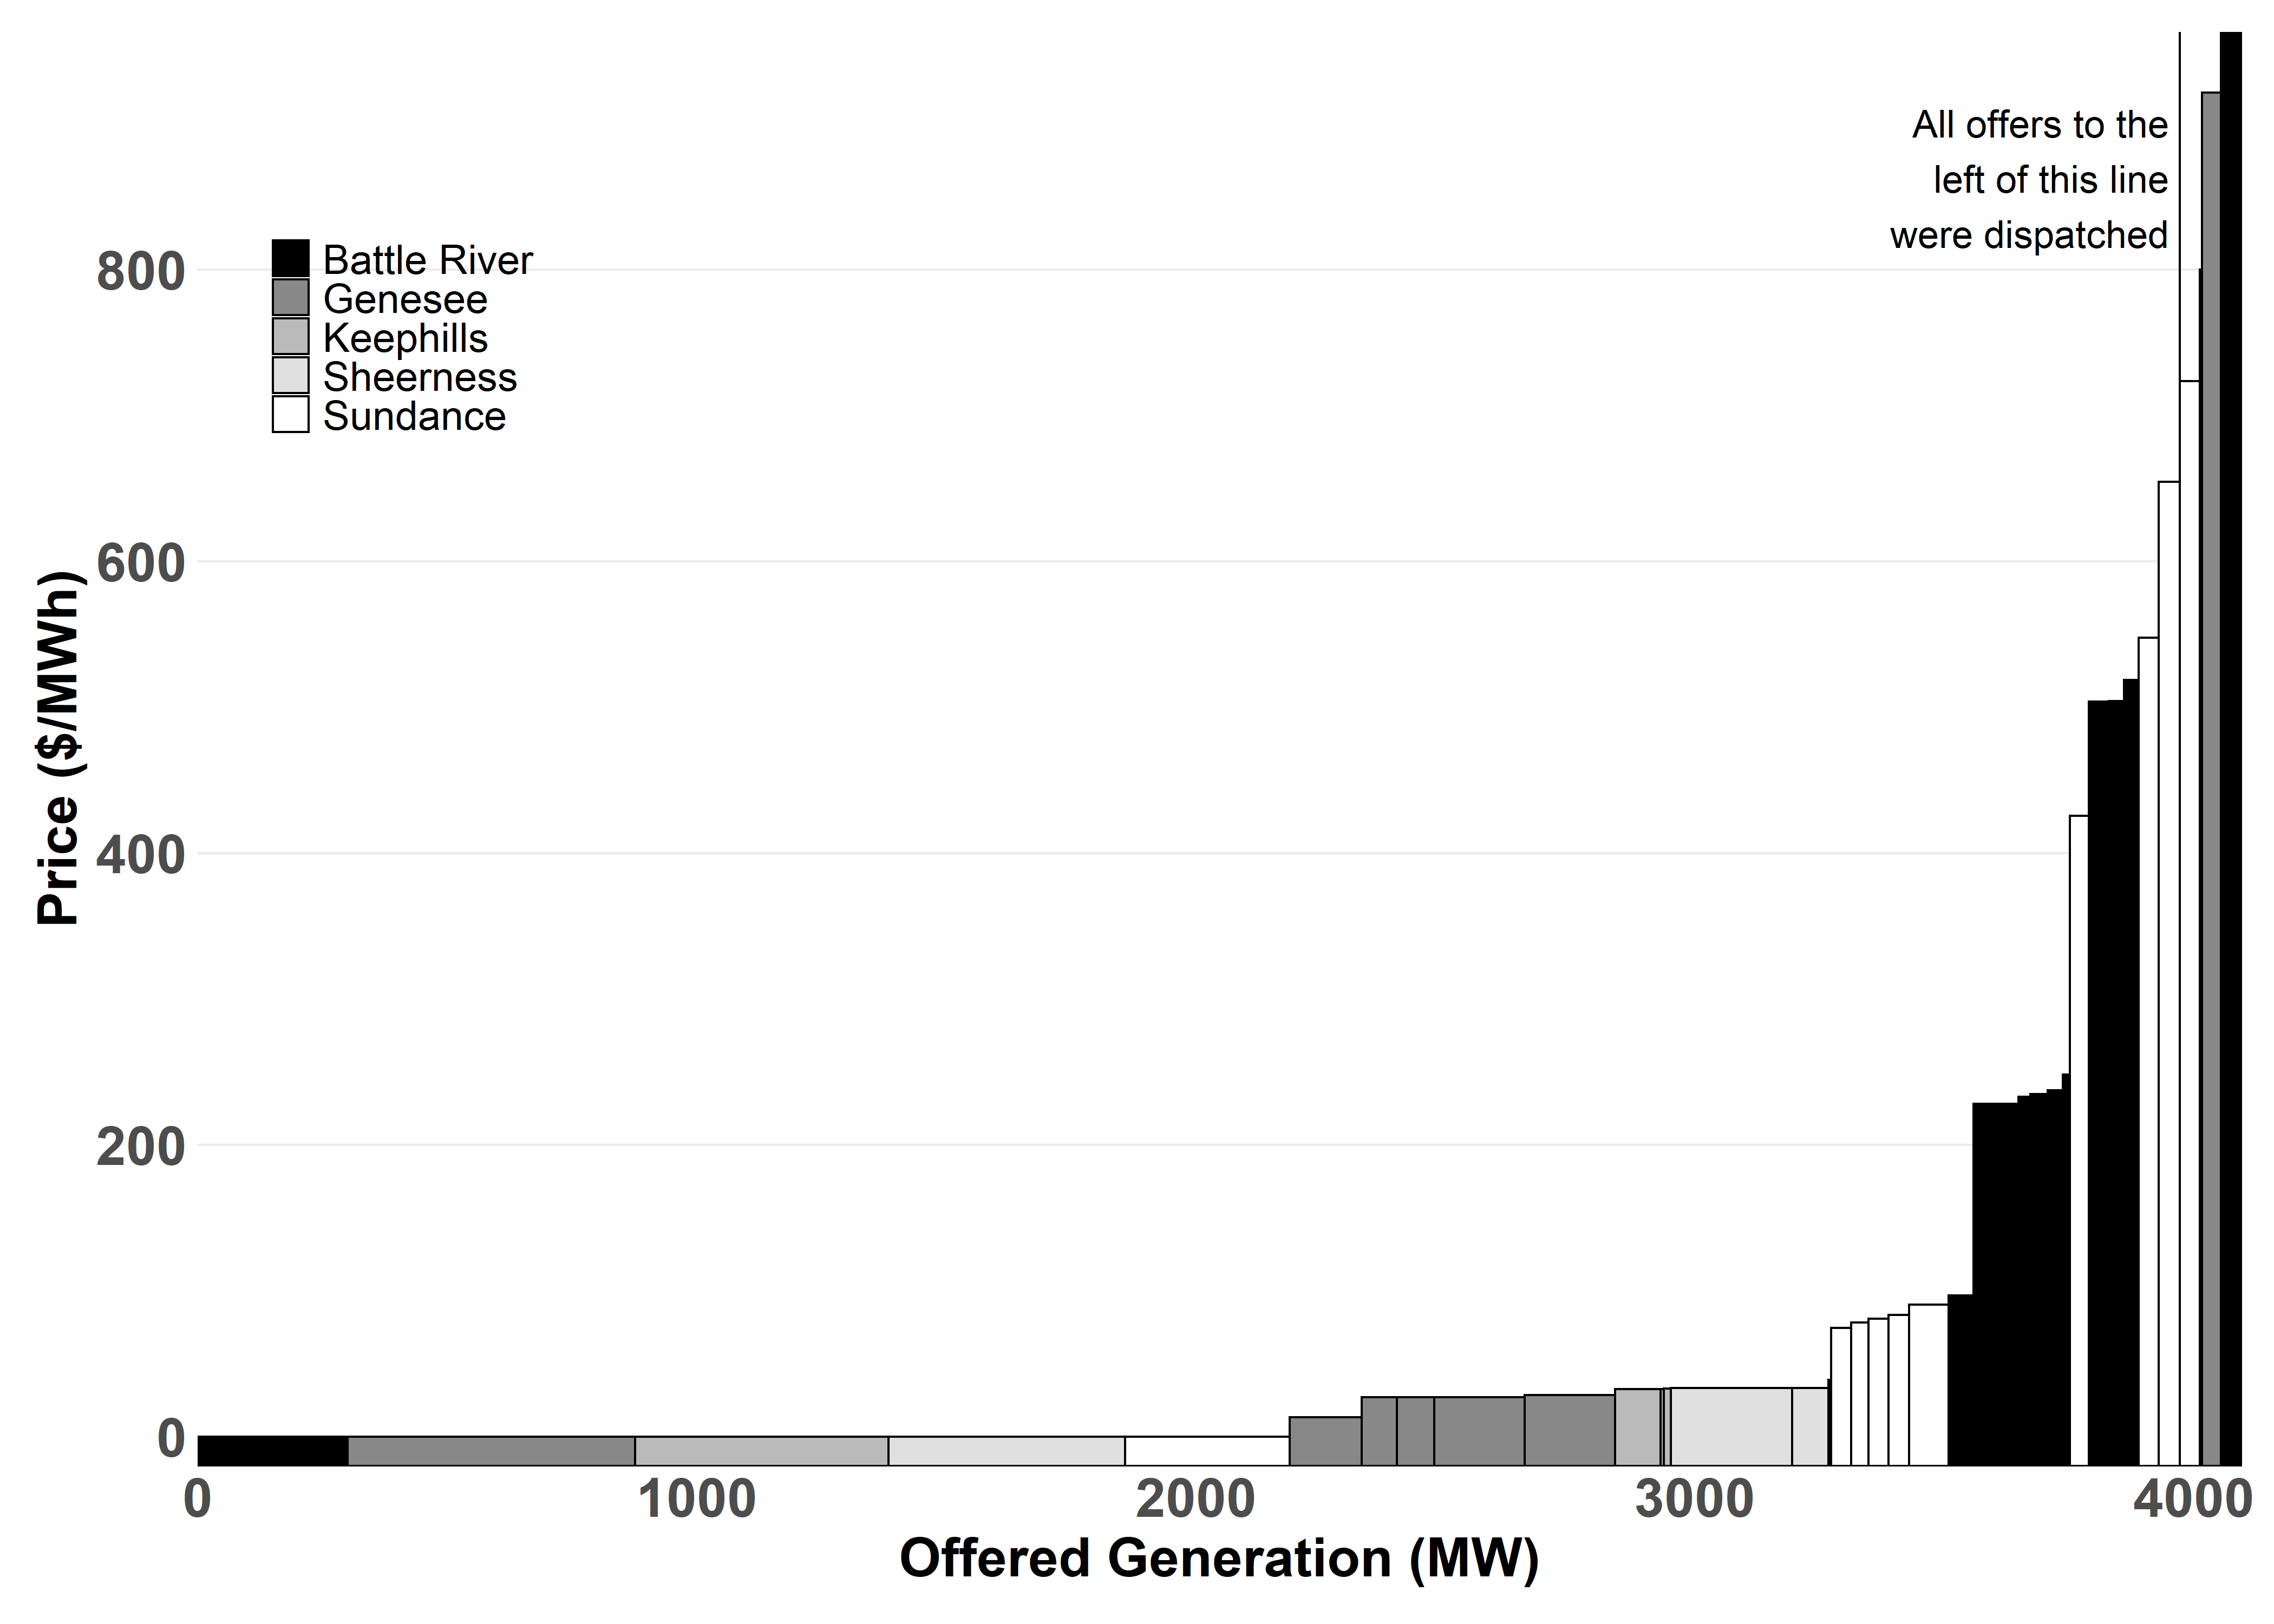
\includegraphics[width=.9\textwidth]{../images/coal_merit.png}
        %\caption{$dt=0.1$}
        %\label{fig:prob1_6_2}
    \end{minipage}%
    \begin{minipage}{0.5\textwidth}
        \centering
        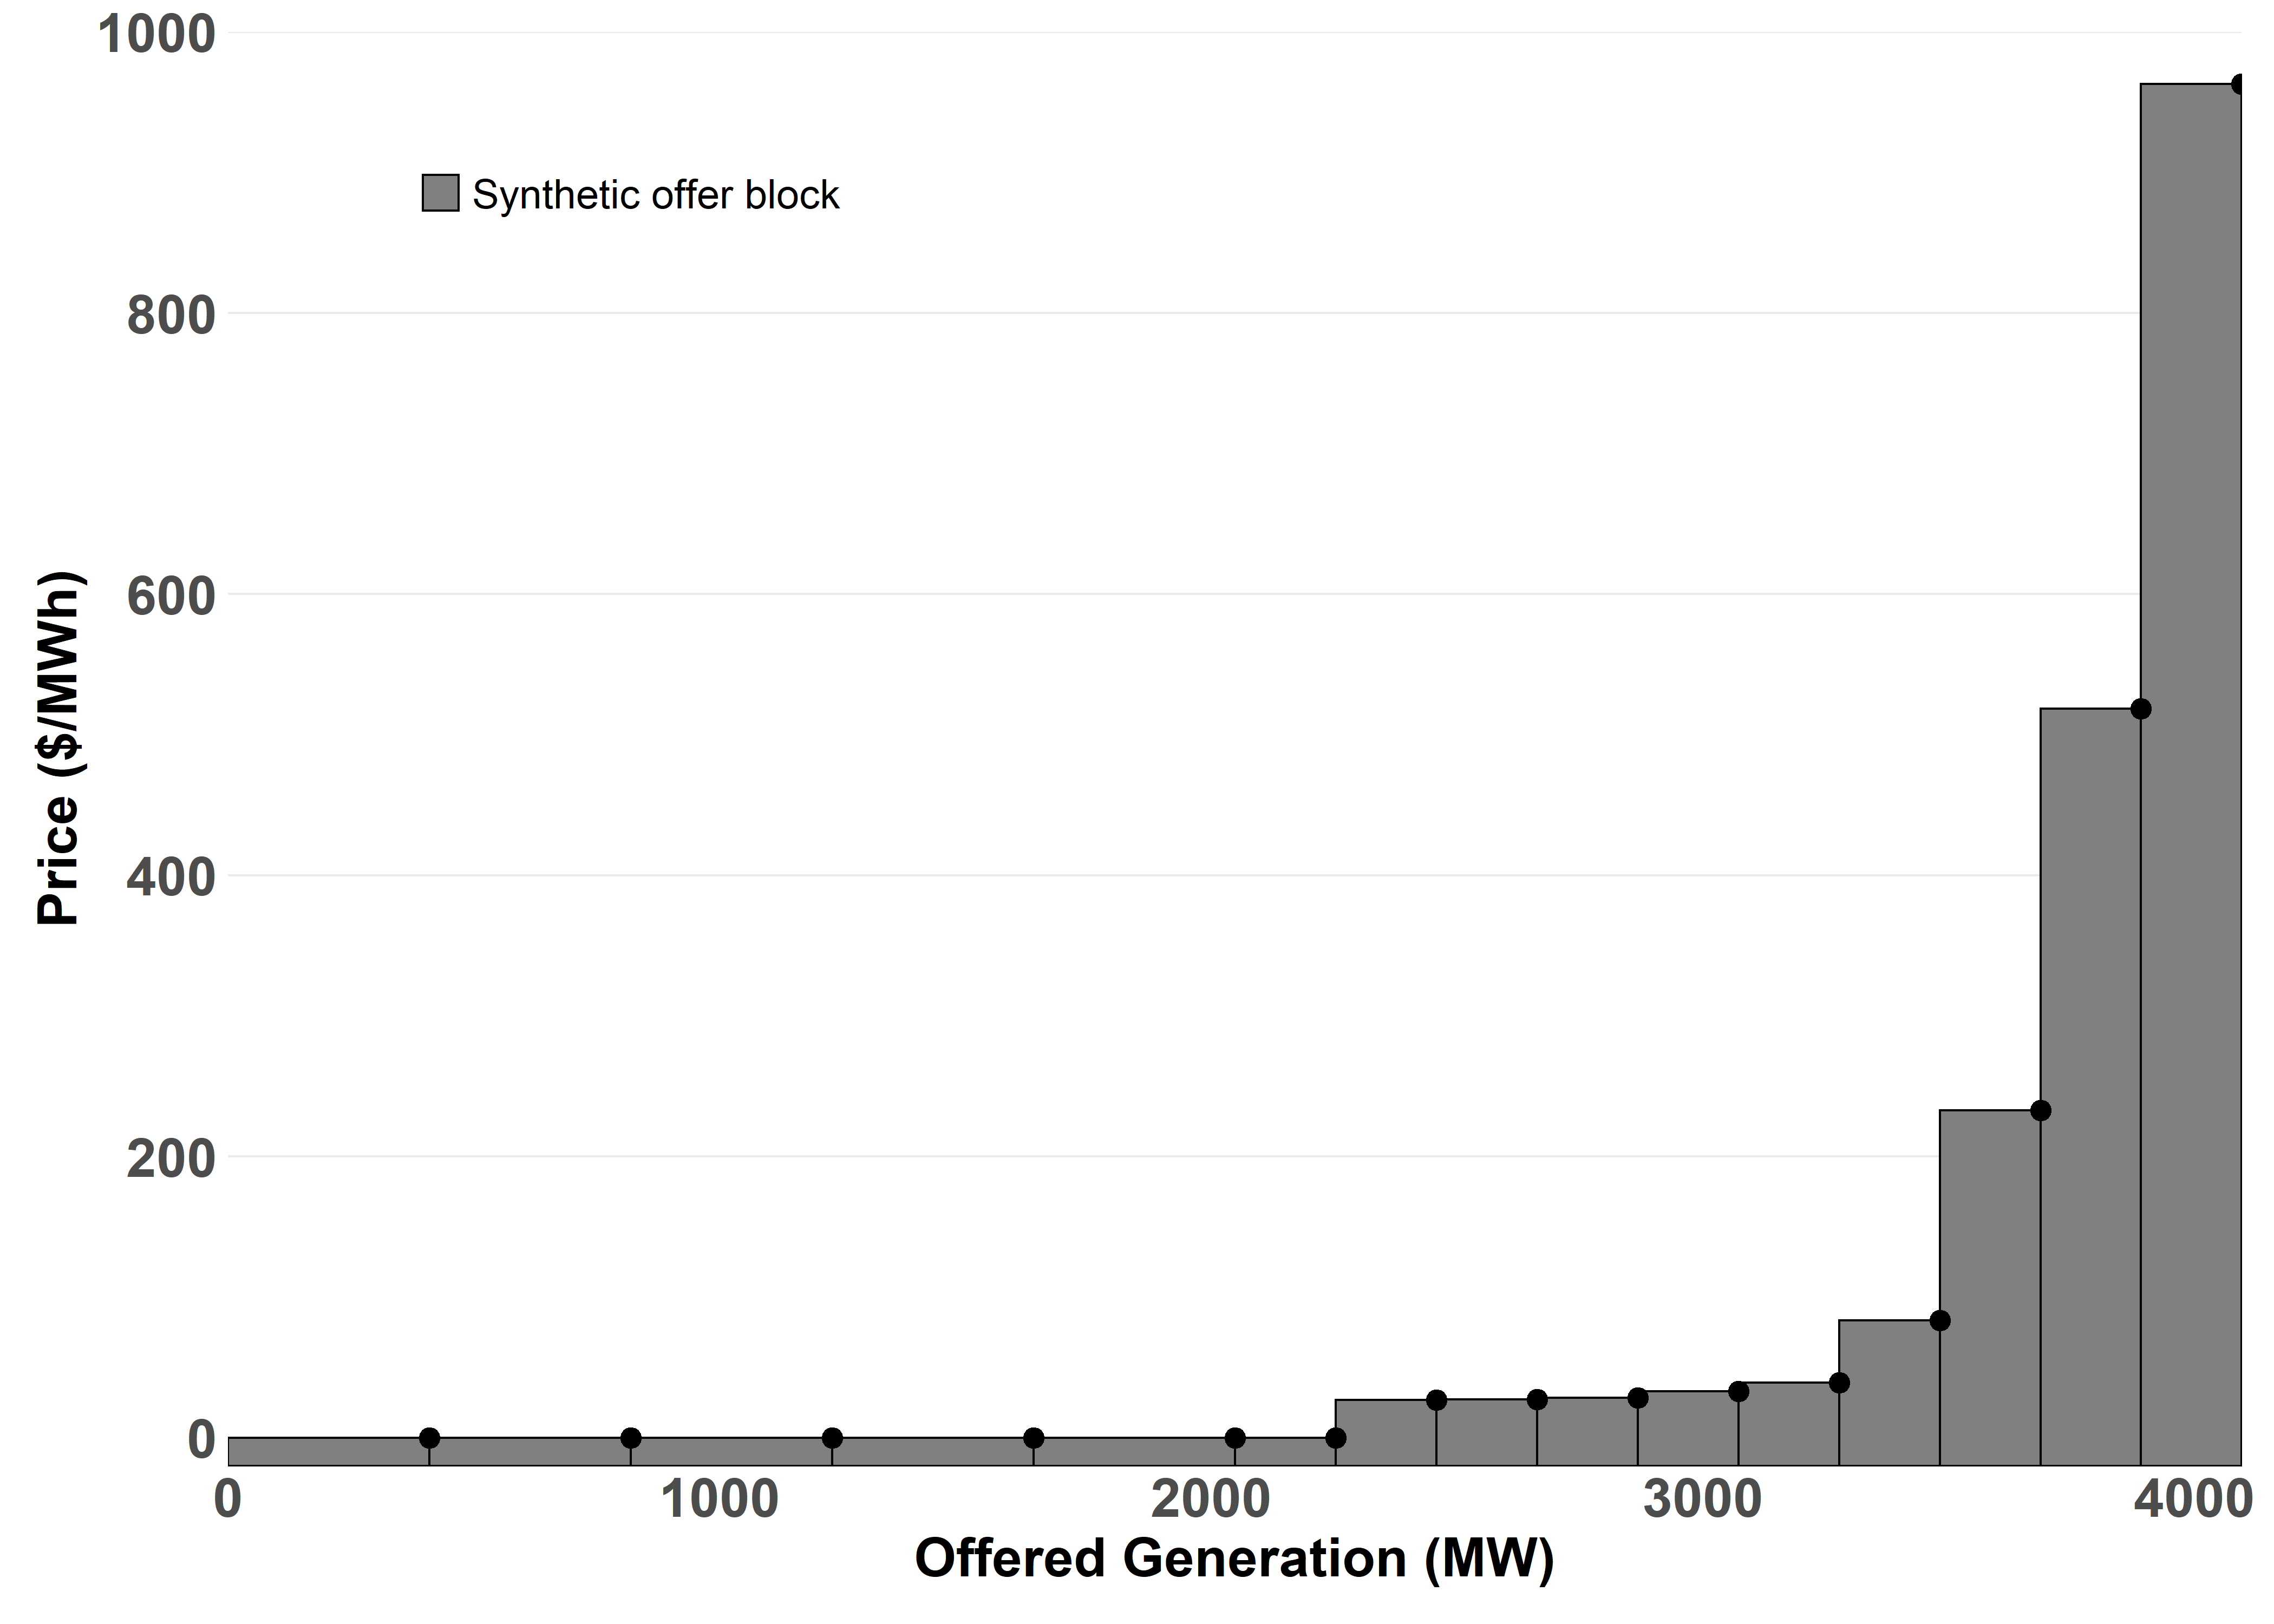
\includegraphics[width=.9\textwidth]{../images/coal_synth_merit}
        %\caption{$dt =$}
        %\label{fig:prob1_6_1}
    \end{minipage}
    \caption{Observed coal facility merit order (left panel) and synthetic coal merit order (right panel) for February 4, 2019 at 7pm. For each hour, we convert the empirical merit order to a step function, and then extract the y-intercept as at 14 unique percentiles of total offered power in that hour, using 5\% increments in the upper half of the merit order.}
    \label{fig:synth_merit}
\end{figure}

There is a lot of day-to-day and hour-to-hour variability in how coal units are offered into the market. Figure \ref{fig:synth_coal_2019}, which shows all of the 7pm merit orders (left panel) and their synthetic equivalents based only on the sample points, along with the average synthetic merit order for the last year of our sample (right panel), provides a sense of the variability in our sample. Similar variability exists in the offers of generation from other dispatchable sources.\footnote{See online graphical appendix, Figure A1, for a similar Figure for all dispatchable generating source types.} Figure \ref{fig:synth_coal_2019} shows the degree to which changes in total offered capacity would skew our results if we attempted to base our analysis on offered megawatts. Instead, by using percentiles of offered capacity as our units of measure, we can more cleanly ask how different segments of the supply curve shift vertically in response to different events, while implicitly assuming that the total offered power available in the market in a given hour is independent of the carbon pricing policy on offer at the time.

\begin{figure}[!htb]
    \centering
    \begin{minipage}{.5\textwidth}
        \centering
        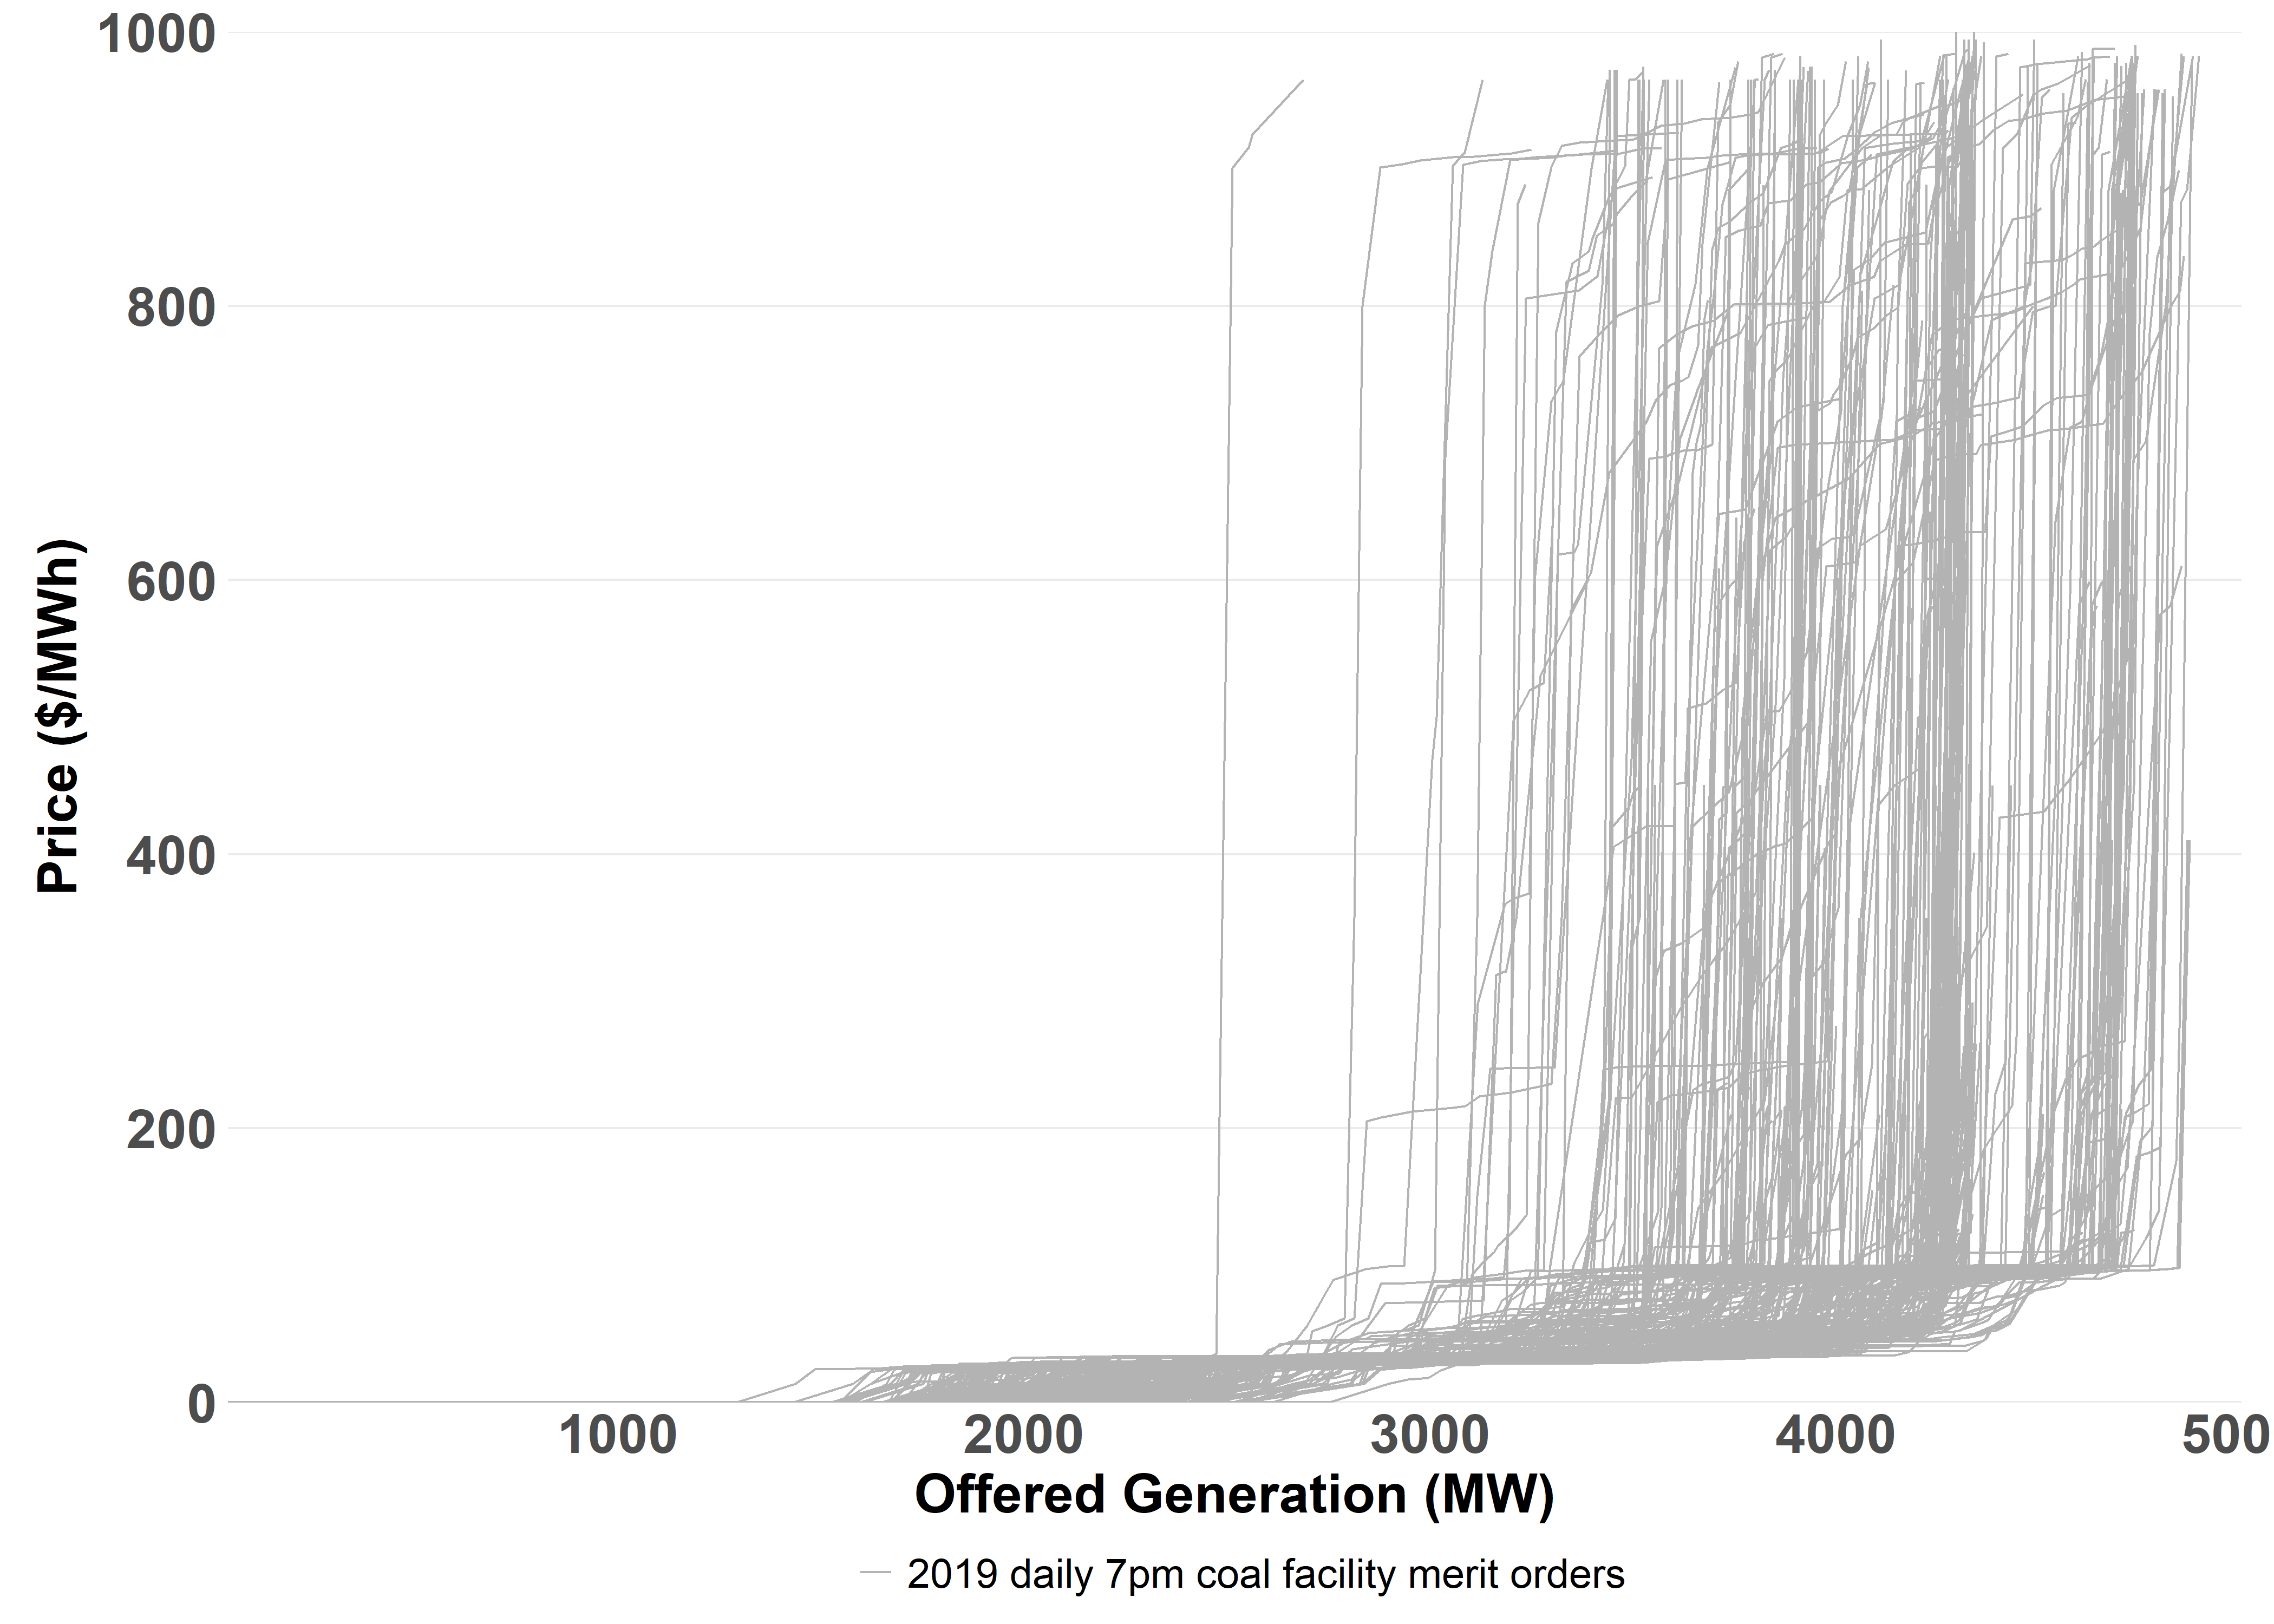
\includegraphics[width=.9\textwidth]{../images/all_coal_merit.png}
        %\caption{$dt=0.1$}
        %\label{fig:prob1_6_2}
    \end{minipage}%
    \begin{minipage}{0.5\textwidth}
        \centering
        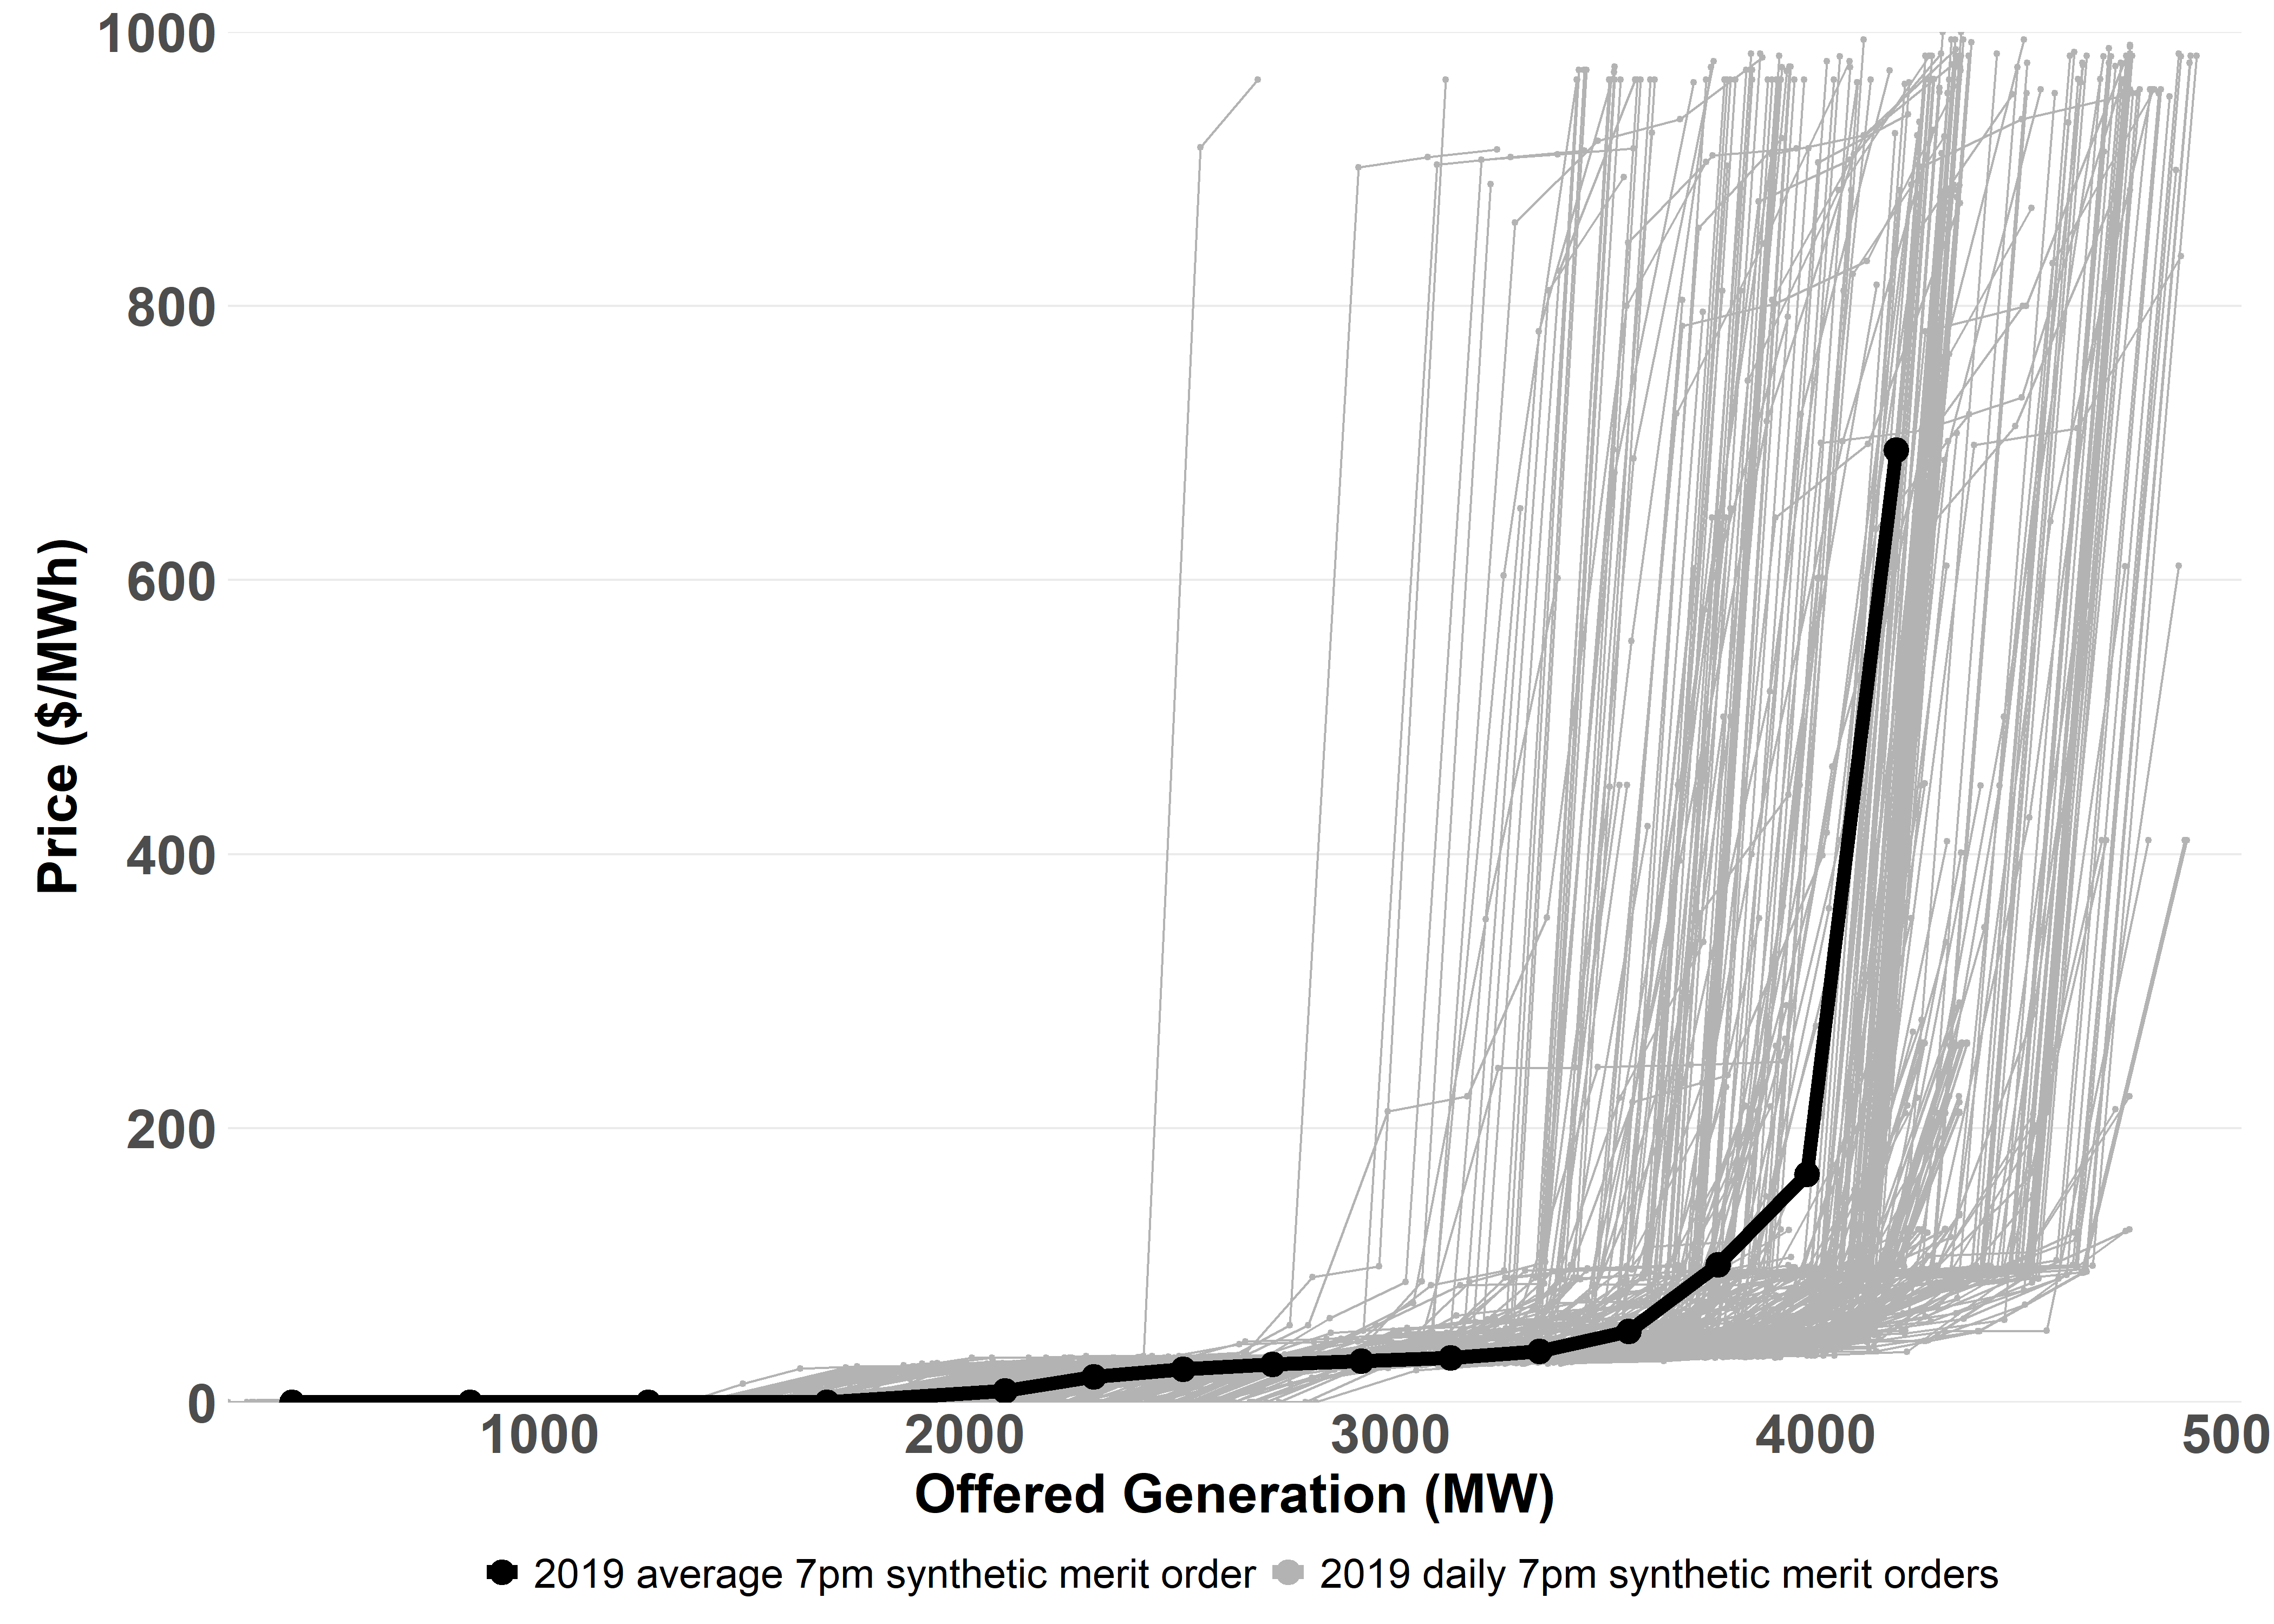
\includegraphics[width=.9\textwidth]{../images/coal_synth_2019}
        %\caption{$dt =$}
        %\label{fig:prob1_6_1}
    \end{minipage}
    \caption{Observed coal facility merit order (left panel) and synthetic coal merit order (right panel) for all of the 7pm hours of 2019.}
    \label{fig:synth_coal_2019}
\end{figure}

For our analysis sample, we create four types of synthetic merit orders. First, for very general results, we characterize the entire merit order using the methodology outlined above. Next, we decompose the results for dispatchable generation types (coal and natural gas plants). We also use the fact that, from 2013 through 2019, the AESO provides offer control by unit as part of their merit order releases. We use this information to construct synthetic supply curves for each of the major participants in the Alberta power market. We also look at the behaviour of some of the largest facilities in the province. This means that we have facility-level, firm- or portfolio-level and market-level synthetic merit orders to analyze.

For parts of our sample, censoring is also an issue. In the Alberta market, negative price offers are not allowed, and offers are capped at \$1000/MWh. This implies that we may under-estimate pass-through where either power offers have a less negative implied value below zero or where the carbon tax leads to a higher true costs of offer above \$1000, as we would not observe either of these effects. To correct for this, we augment our ordinary least squares estimates of pass-through with Tobit estimates with two-sided censoring, estimated via maximum likelihood. We do not find the censoring to have a marked effect on our estimates.


\section{Results and Discussion}

\subsection{Market-wide impacts}
The most general results derive from the analysis of the market as a whole. Here, we are calculating, for each hour of our sample, the supply curve of power offered into the market which we summarize using a step function with 15 points of support mapping offers at given percentiles of total power offers. At each of these points of support, we also track the marginal carbon pricing cost and marginal output-based allocation value along with other market and environmental variables. When we consider only the net marginal cost of carbon pricing (the hourly carbon charge net the hourly output-based allocation of credits), we find a pattern that will be familiar through the remainder of the results in this paper. As shown in Figure \ref{fig:net_all}, there is no impact of carbon pricing on offers at the low end of the merit, as this range is characterized by zero dollar offers in all hours of the year. The mid-merit range is where we see most of the impacts, and these are intuitive although smaller than might be expected. Our study design is such that, if the costs of carbon pricing were fully passed-through to offers, and if we measured we would expect to see an estimated coefficient exactly equal to 1 on the impact of carbon pricing. The maximum carbon price pass-through appears at the 60th through 70th percentile of offered power, with the maximum share of net carbon costs passed through to offered prices at just less than 40\%. In this formulation, there is no statistical support for the contention that carbon prices are, on average, fully passed-through at the margin in electricity markets.

\begin{figure}[!htb]
    \centering
     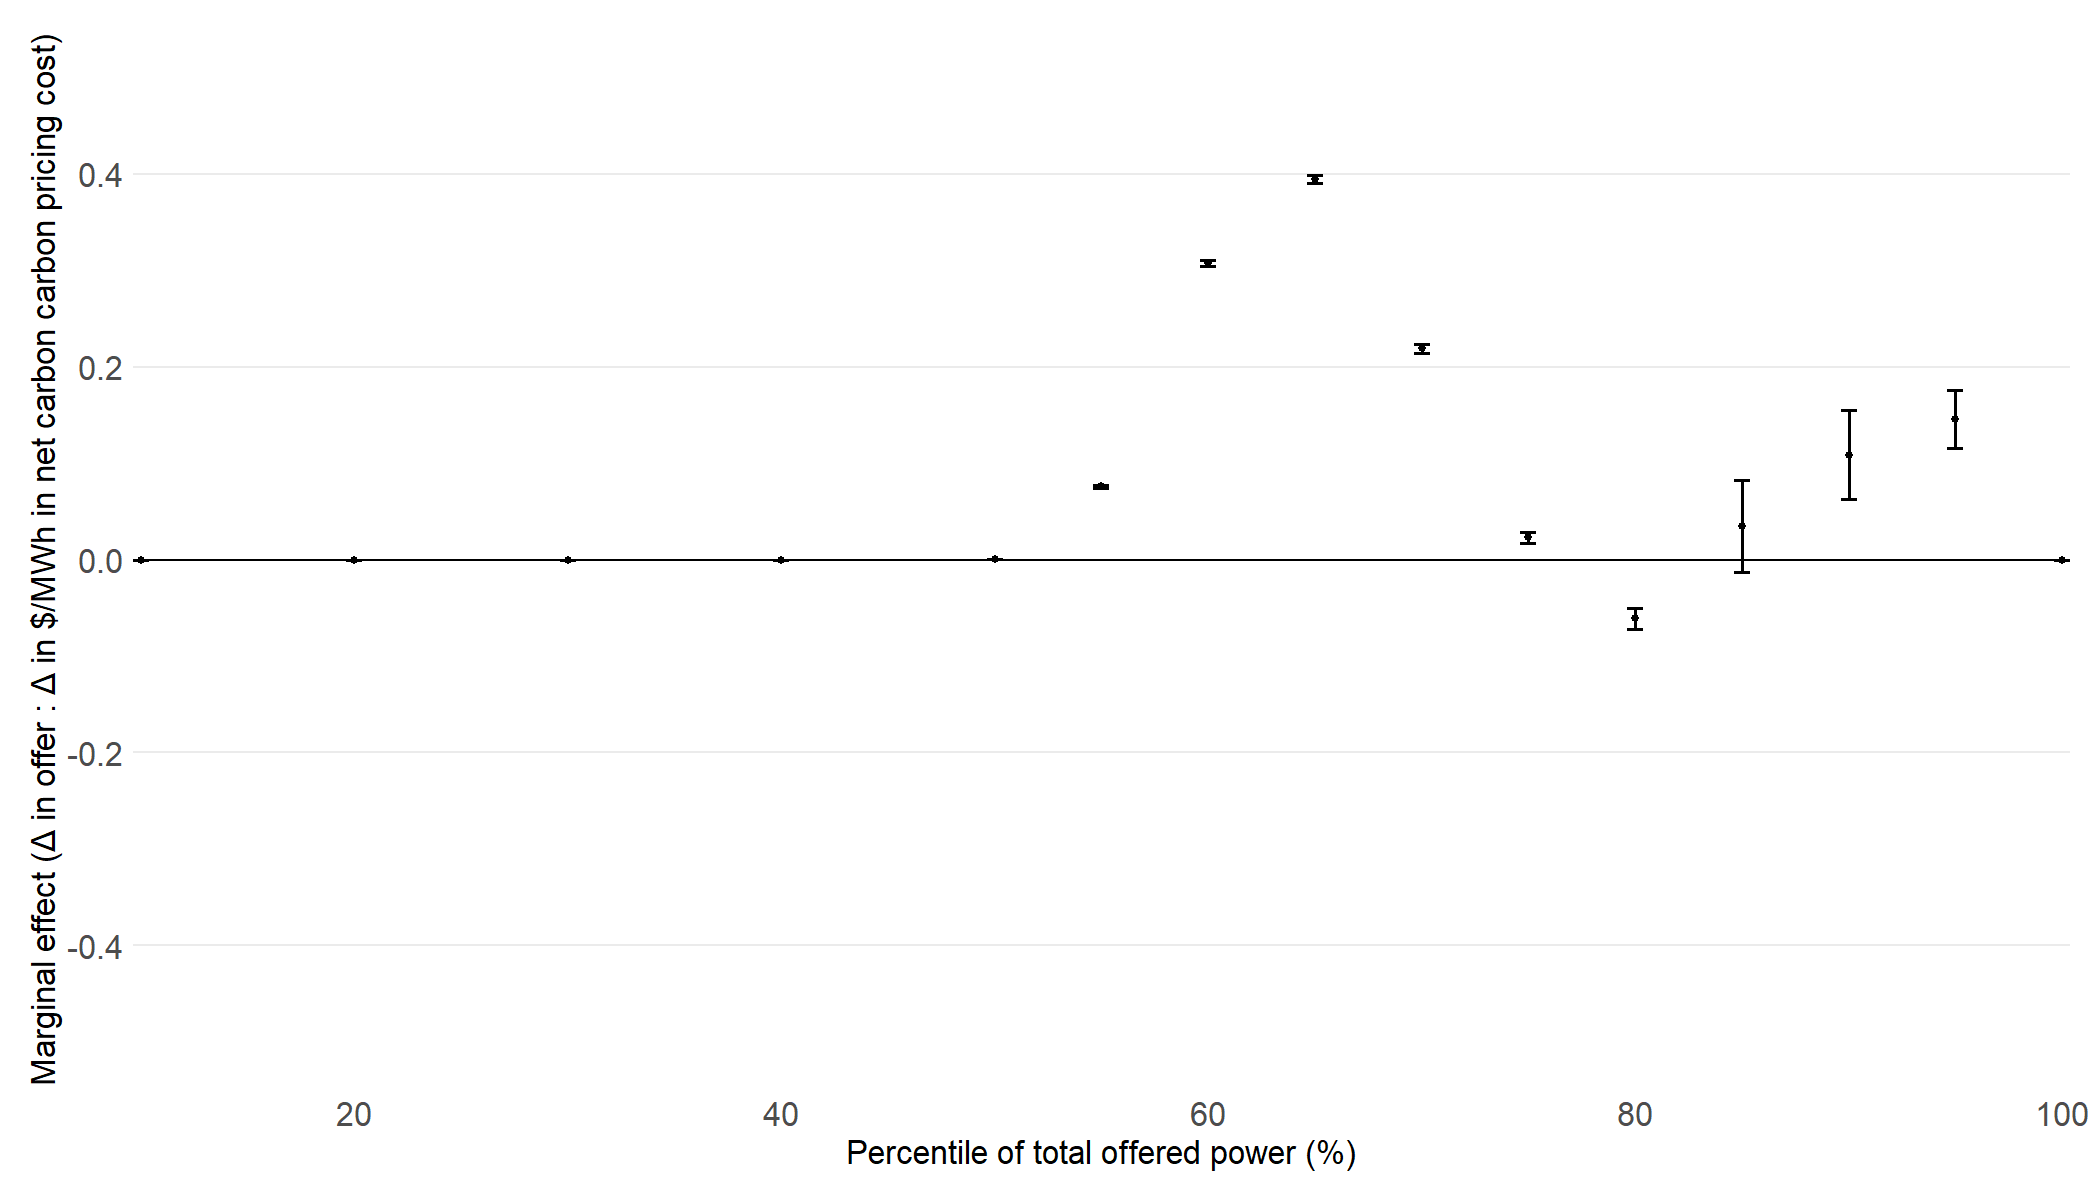
\includegraphics[width=.9\textwidth]{../images/all_plants_net.png}
    \caption{Estimated marginal effect of net carbon charges on power offers, all plant types and all hours. Error bars denote 95\% confidence intervals}
    \label{fig:net_all}
\end{figure}


Since the marginal cost of offered power becomes less elastic (the slope of the merit order increases) at higher levels of offered power, it's reasonable to expect that the pass-through would be altered at peak hours when demand for power is higher. In our base regression shown above, we include a peak-hours factor within the regression, but do not interact that term with carbon costs. In Figure \ref{fig:net_peak}, we re-calculate the regression results allowing the carbon pricing effect to vary across peak hours and non-peak hours, and we do find intuitive although only weakly statistically significant changes. The net effect of the carbon pricing cost is positive across all by the 80th percentile sampling point, with the largest effects occurring slightly lower in the merit order in off-peak hours, and we also see statistically significant pass-through of net carbon costs at the upper end of the merit order as well.

\begin{figure}[!htb]
    \centering
     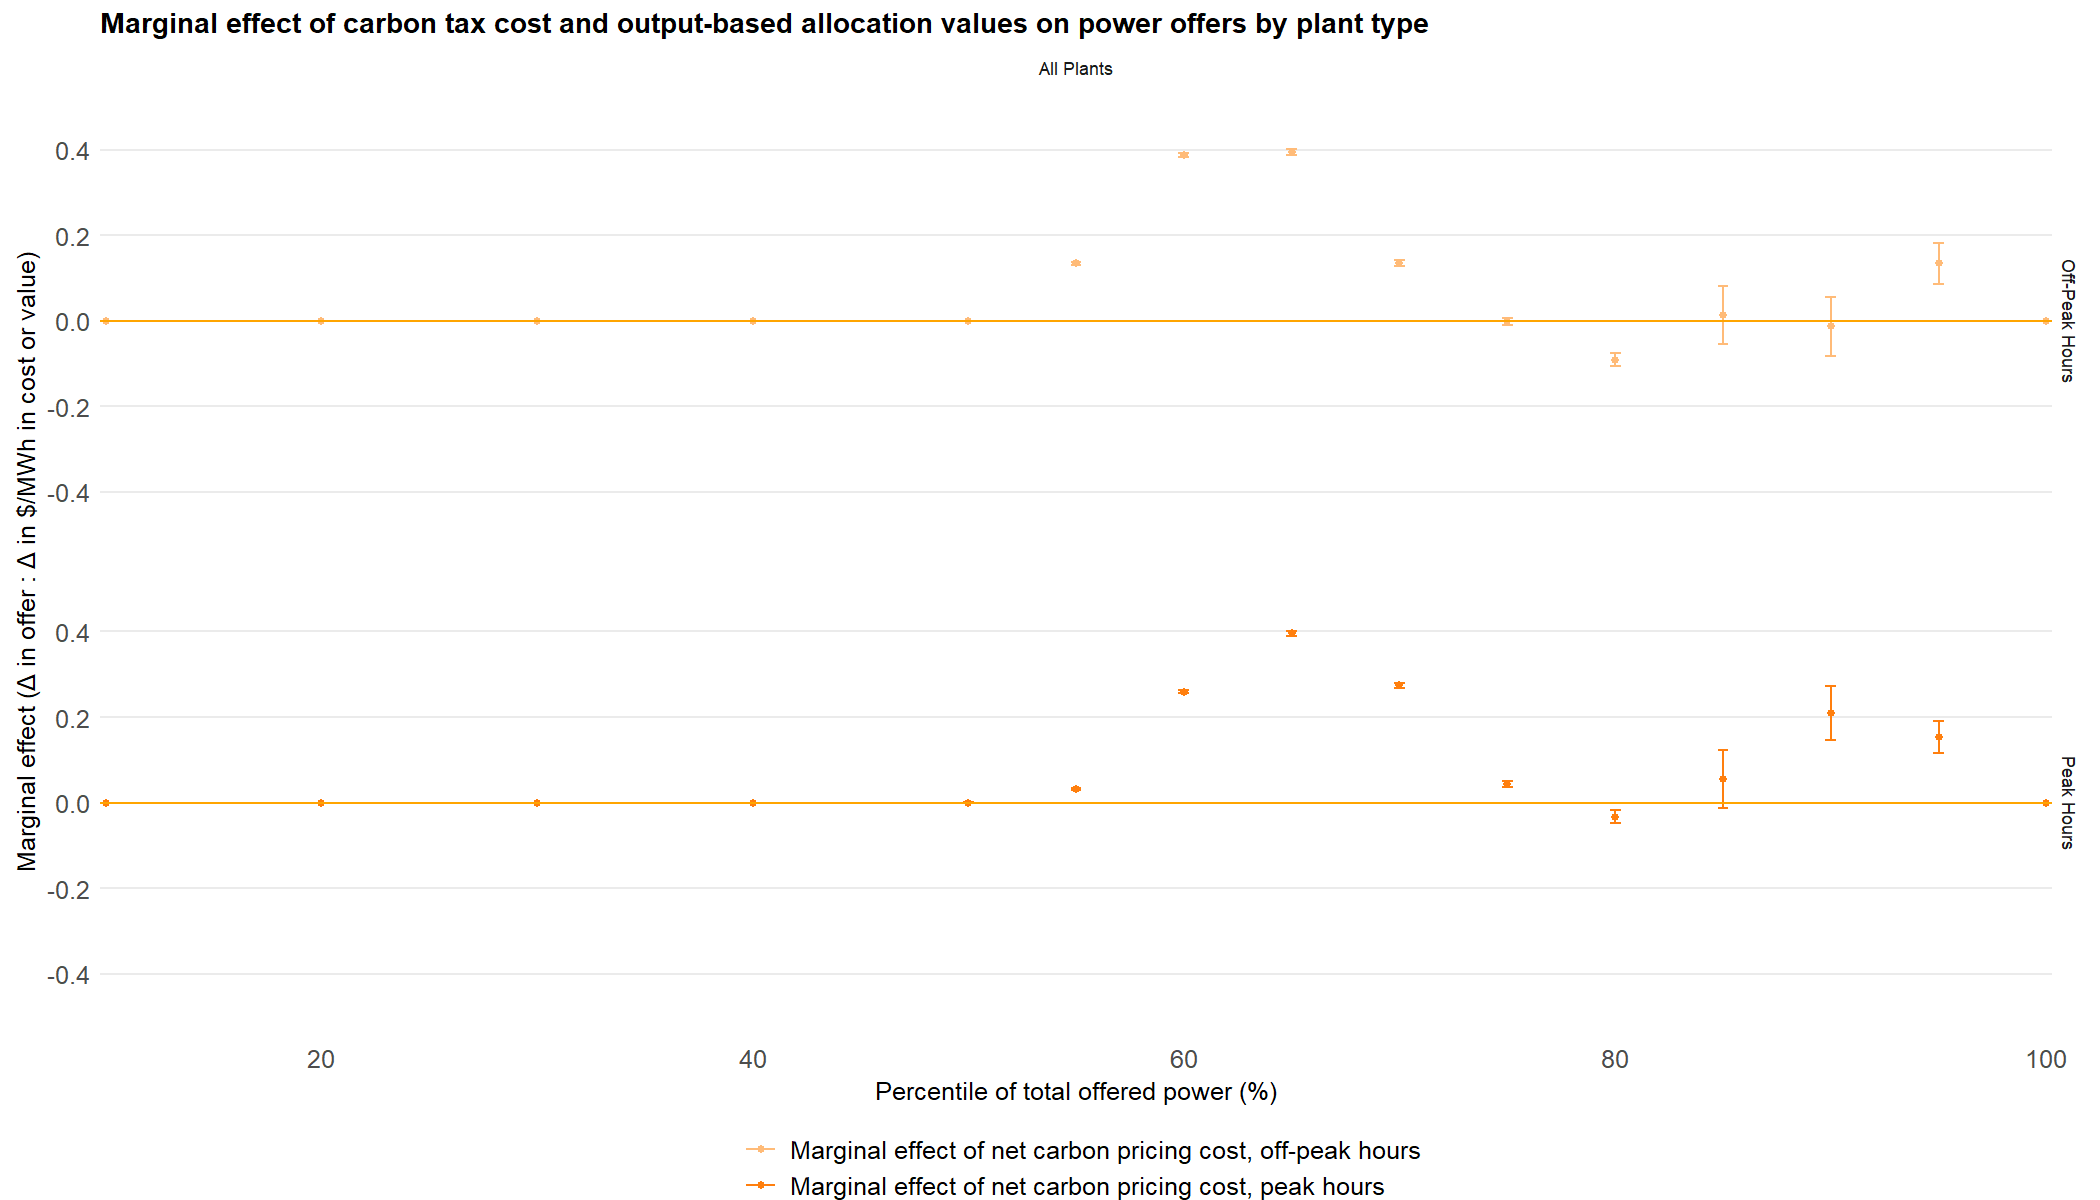
\includegraphics[width=.9\textwidth]{../images/all_plants_net_peak.png}
    \caption{Estimated marginal effect of net carbon charges on power offers, all plant types and all hours. Error bars denote 95\% confidence intervals}
    \label{fig:net_peak}
\end{figure}


Our data allows a decomposition of the net effect of carbon pricing into a carbon tax and an OBA effect, although with some important caveats. Recall that what we are calling a carbon tax effect in any given hour is the average annual carbon tax per MWh of generation, and so we will miss impacts that occur as a result of hourly ramping or other intensive margin conditions. Also, for some facilities, we have emissions-intensity data at the aggregate level, and in some cases a facility may include as many as six generating units. Where the average emissions intensity varies across units within the facility, we will measure the individual unit intensities with error as well. As such, we knot that our marginal effective costs of carbon pricing are measured imprecisely. The output-based allocations are consistent through the year on a per-MWh basis, and are determined at the facility level, so we have more accurate measures of these values in our data. Again, our estimation strategy is such that a coefficient with an absolute value of 1 where perfect pass-through has occurred, with a value of negative 1 for the full pass through of an output-based allocation to lower offers and a value of 1 for the full pass-through of carbon taxes to higher power offers.

Our results, shown in Figure \ref{fig:decomp_all_hours}, mostly reflect an intuitive decomposition of the results derived based on net values, with a few exceptions. Again, we see no impact below the 50th percentile of offered power, and in the mid-merit, an increased in offered prices as marginal carbon prices increase, but with less than full pass through. In the upper merit, it's clear that factors other than carbon prices are driving offers, and we see a positive impact of carbon prices with varied impacts of output-based allocations, each estimated much less precisely than the mid-merit impacts.


\begin{figure}[!htb]
    \centering
     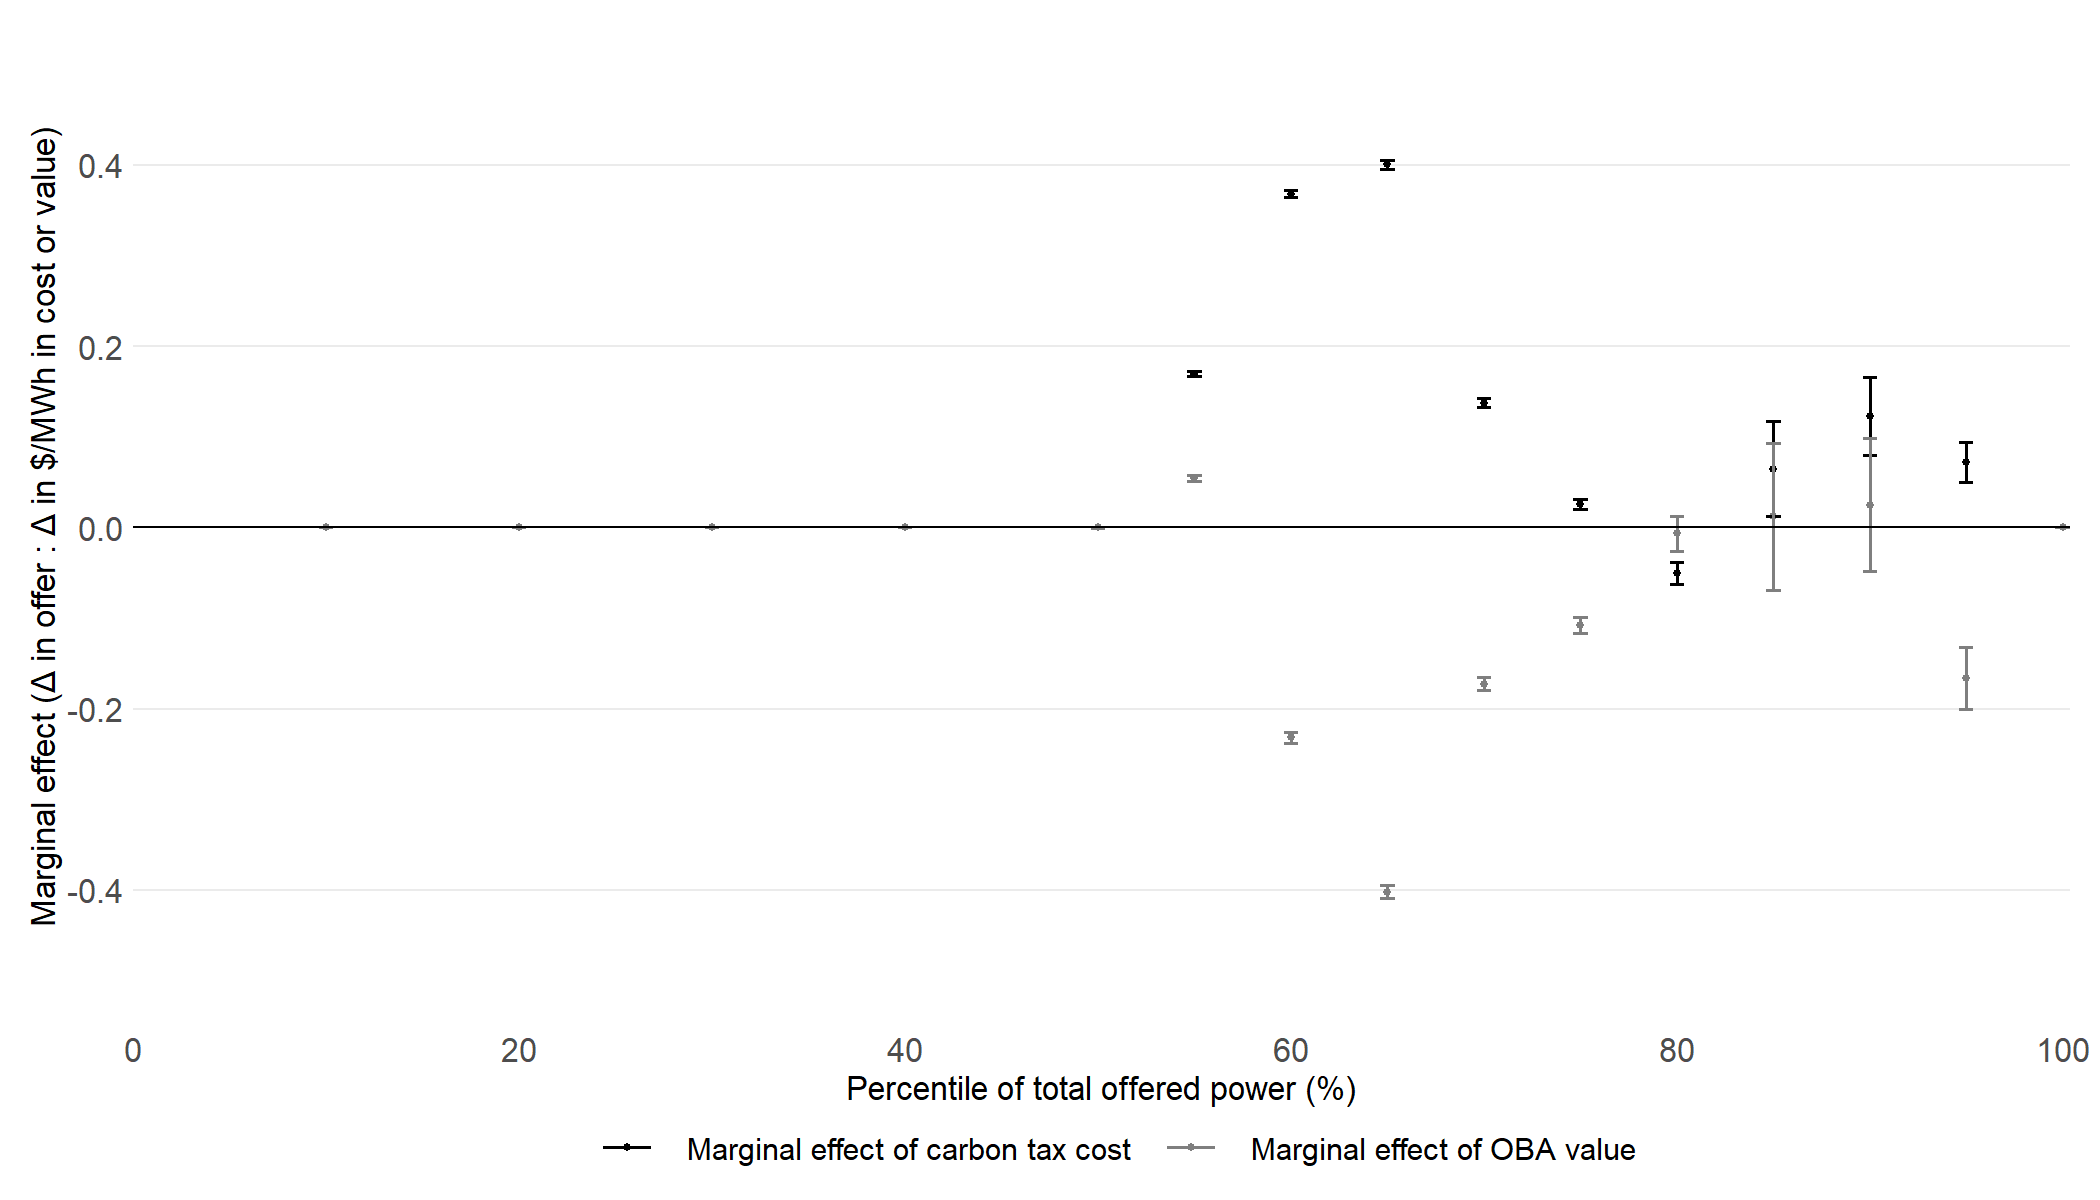
\includegraphics[width=.9\textwidth]{../images/all_plants_no_peaks.png}
    \caption{Estimated marginal effect of net carbon charges on power offers, all plant types and all hours. Error bars denote 95\% confidence intervals}
    \label{fig:decomp_all_hours}
\end{figure}

These results are consistent if a decomposition by peak- vs. off-peak hours is introduced, as shown in Figure \ref{fig:decomp_peaks}. The impact of carbon pricing is always statistically greater than or equal to zero, with a maximum pass-through of approximately 40\% of average carbon costs in the mid-merit, and less elsewhere. In peak hours, the pass-through is smaller in the 50th to 60th percentiles, and larger in the 60th to 75th percentiles, with a similar 40\% maximum pass-through. Carbon price pass-through remains low in the 80th percentile, and increases in the upper merit during peak hours, while being close to zero in off-peak hours except at the extreme top of the merit order. The upper-merit impacts of OBAs are counter-intuitive, especially at peak hours, with estimates suggesting that higher offers have occurred with more valuable OBAs in the 85th to 95th percentiles of power offers in peak hours.


\begin{figure}[!htb]
    \centering
     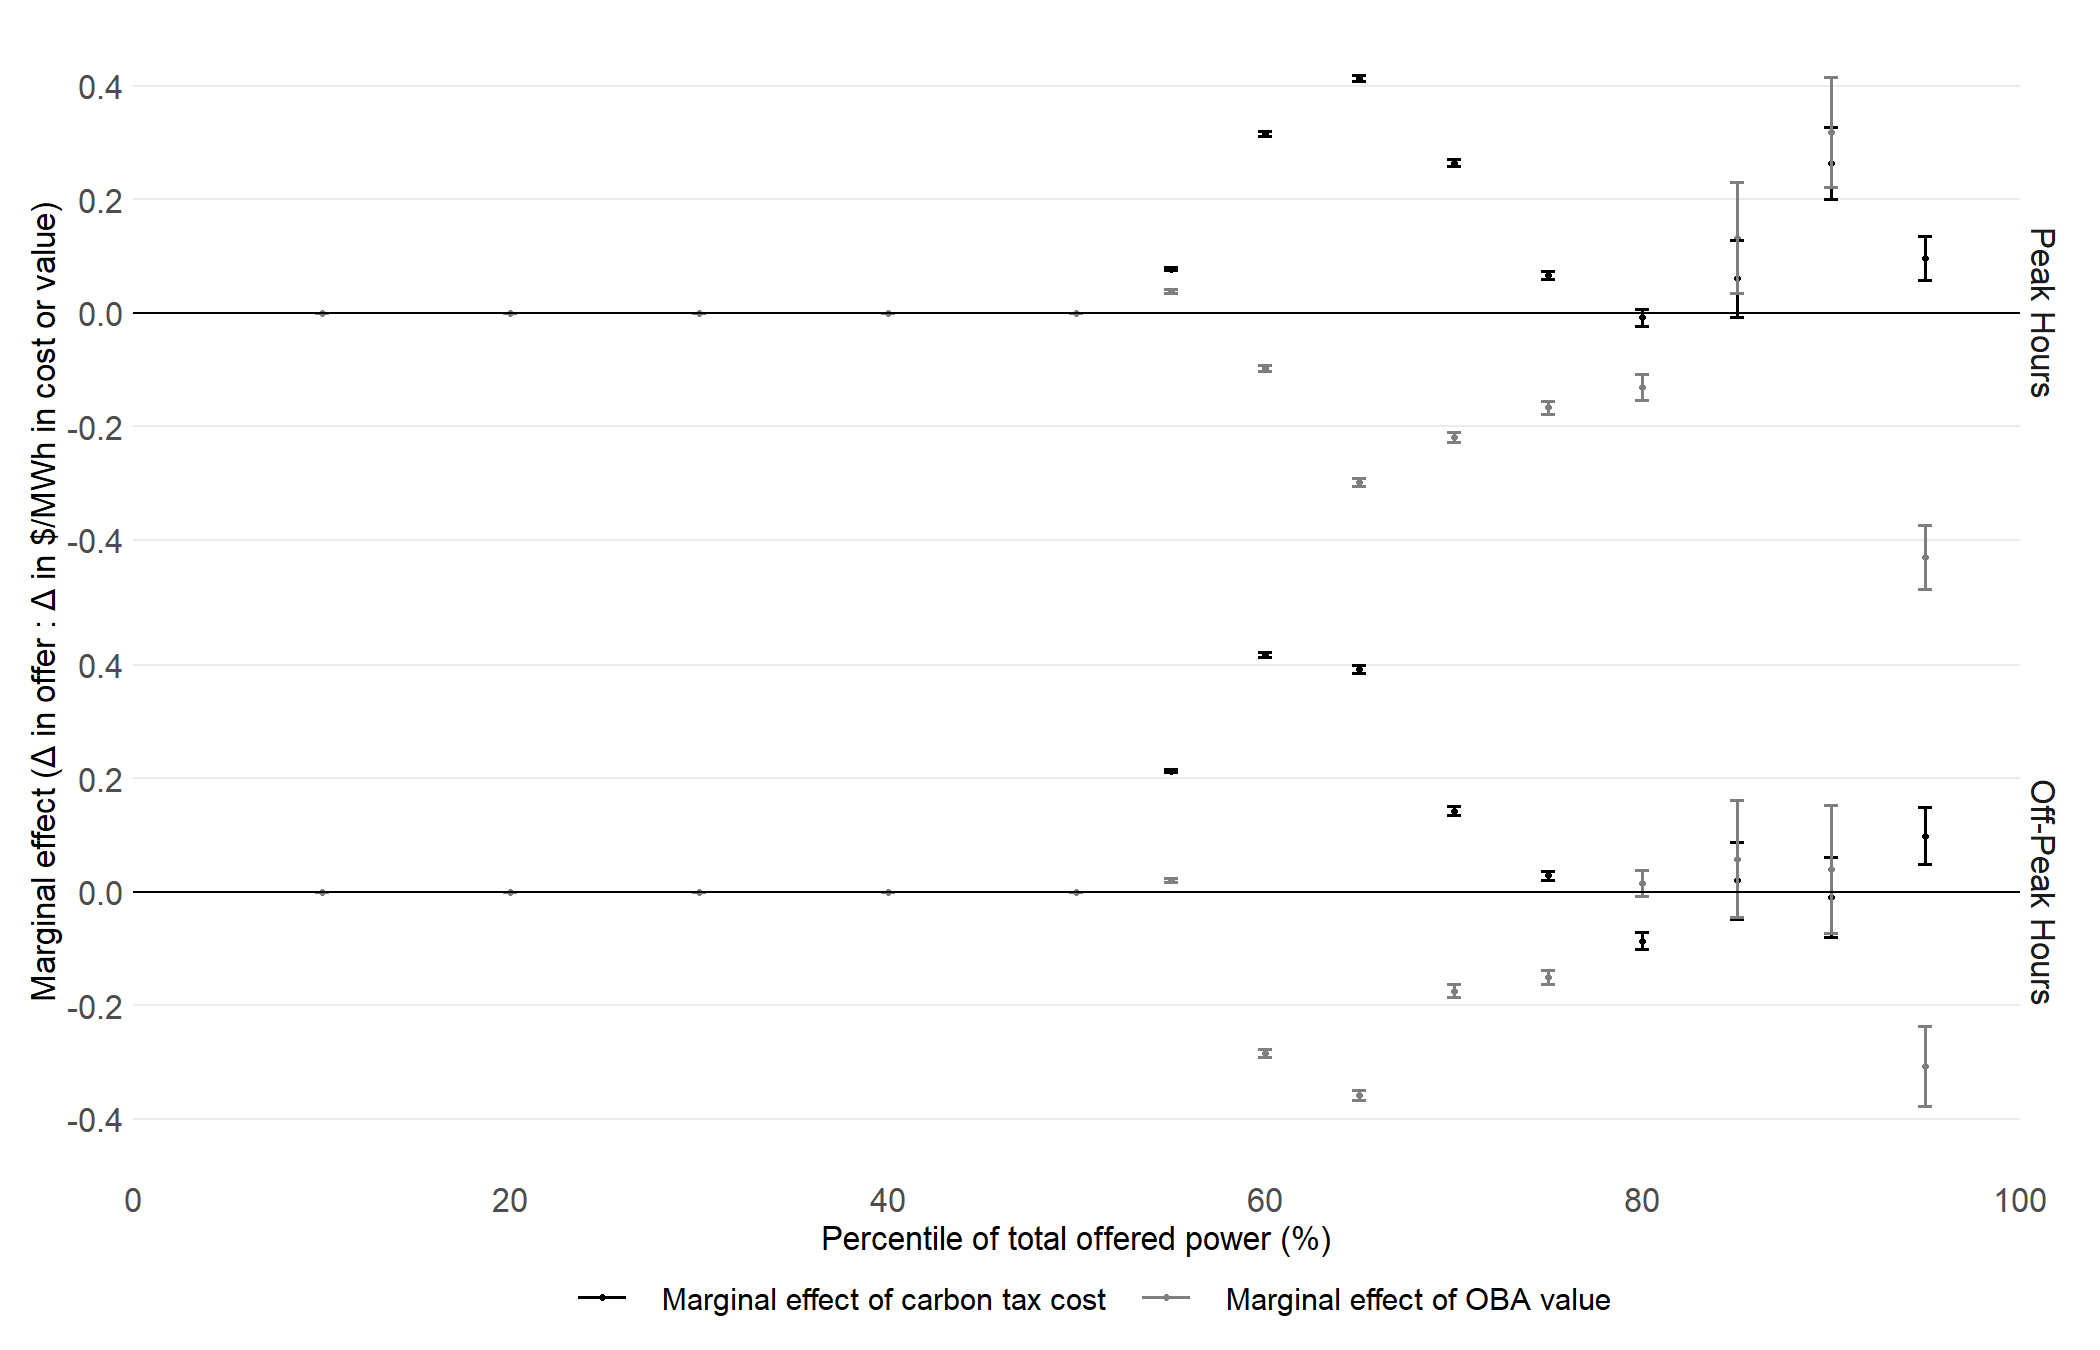
\includegraphics[width=.9\textwidth]{../images/all_plants.png}
    \caption{Estimated marginal effect of net carbon charges on power offers, all plant types. Error bars denote 95\% confidence intervals}
    \label{fig:decomp_peaks}
\end{figure}


\subsection{Impacts By Generator Type}
We know that different generator types tend to offer their power into the market in different ways, and we decompose our key results by plant type, concentrating on the fossil fuel generators, with the exception of the combined heat and power plants for whom we do not observe external drivers for power offers. The results by plant type are, in many cases, counter-intuitive. We find first that coal plants do not consistently pass-through carbon costs to their offers. In fact, in the mid-merit, they tend to shade their offers a bit, actually reducing their offers as carbon prices are increased. This is likely as a result of their direct competition with gas-fired power plants which have lower emissions-intensity. In order to remain in the market at their maximum efficiency, it appears that coal plants are not passing through any carbon costs and are, in fact, reducing their offers despite an increase in costs. In the upper ranges of the merit order, coal plants have higher than full pass through, indicating that their offers over the last megawatts of their portfolio increased by more than their net carbon costs during the sample period. This indicates a change in operating stategy, perhaps, from one of \textit{base load} to more peaking behaviour, only operating plants at full capacity when the market price is very high. This is also, likely, an artefact of our assumption of constant emissions intensity of output. If the marginal emissions-intensity of output at the 90th percentile of installed capacity is much higher than in the mid-range of capacity, we would expect our pass-through estimates to appear as though more than 100\% of these costs were being passed-through, although that alone is insufficient to explain offers increasing by 1-3 times the increase in net carbon costs.

\begin{figure}[!htb]
    \centering
     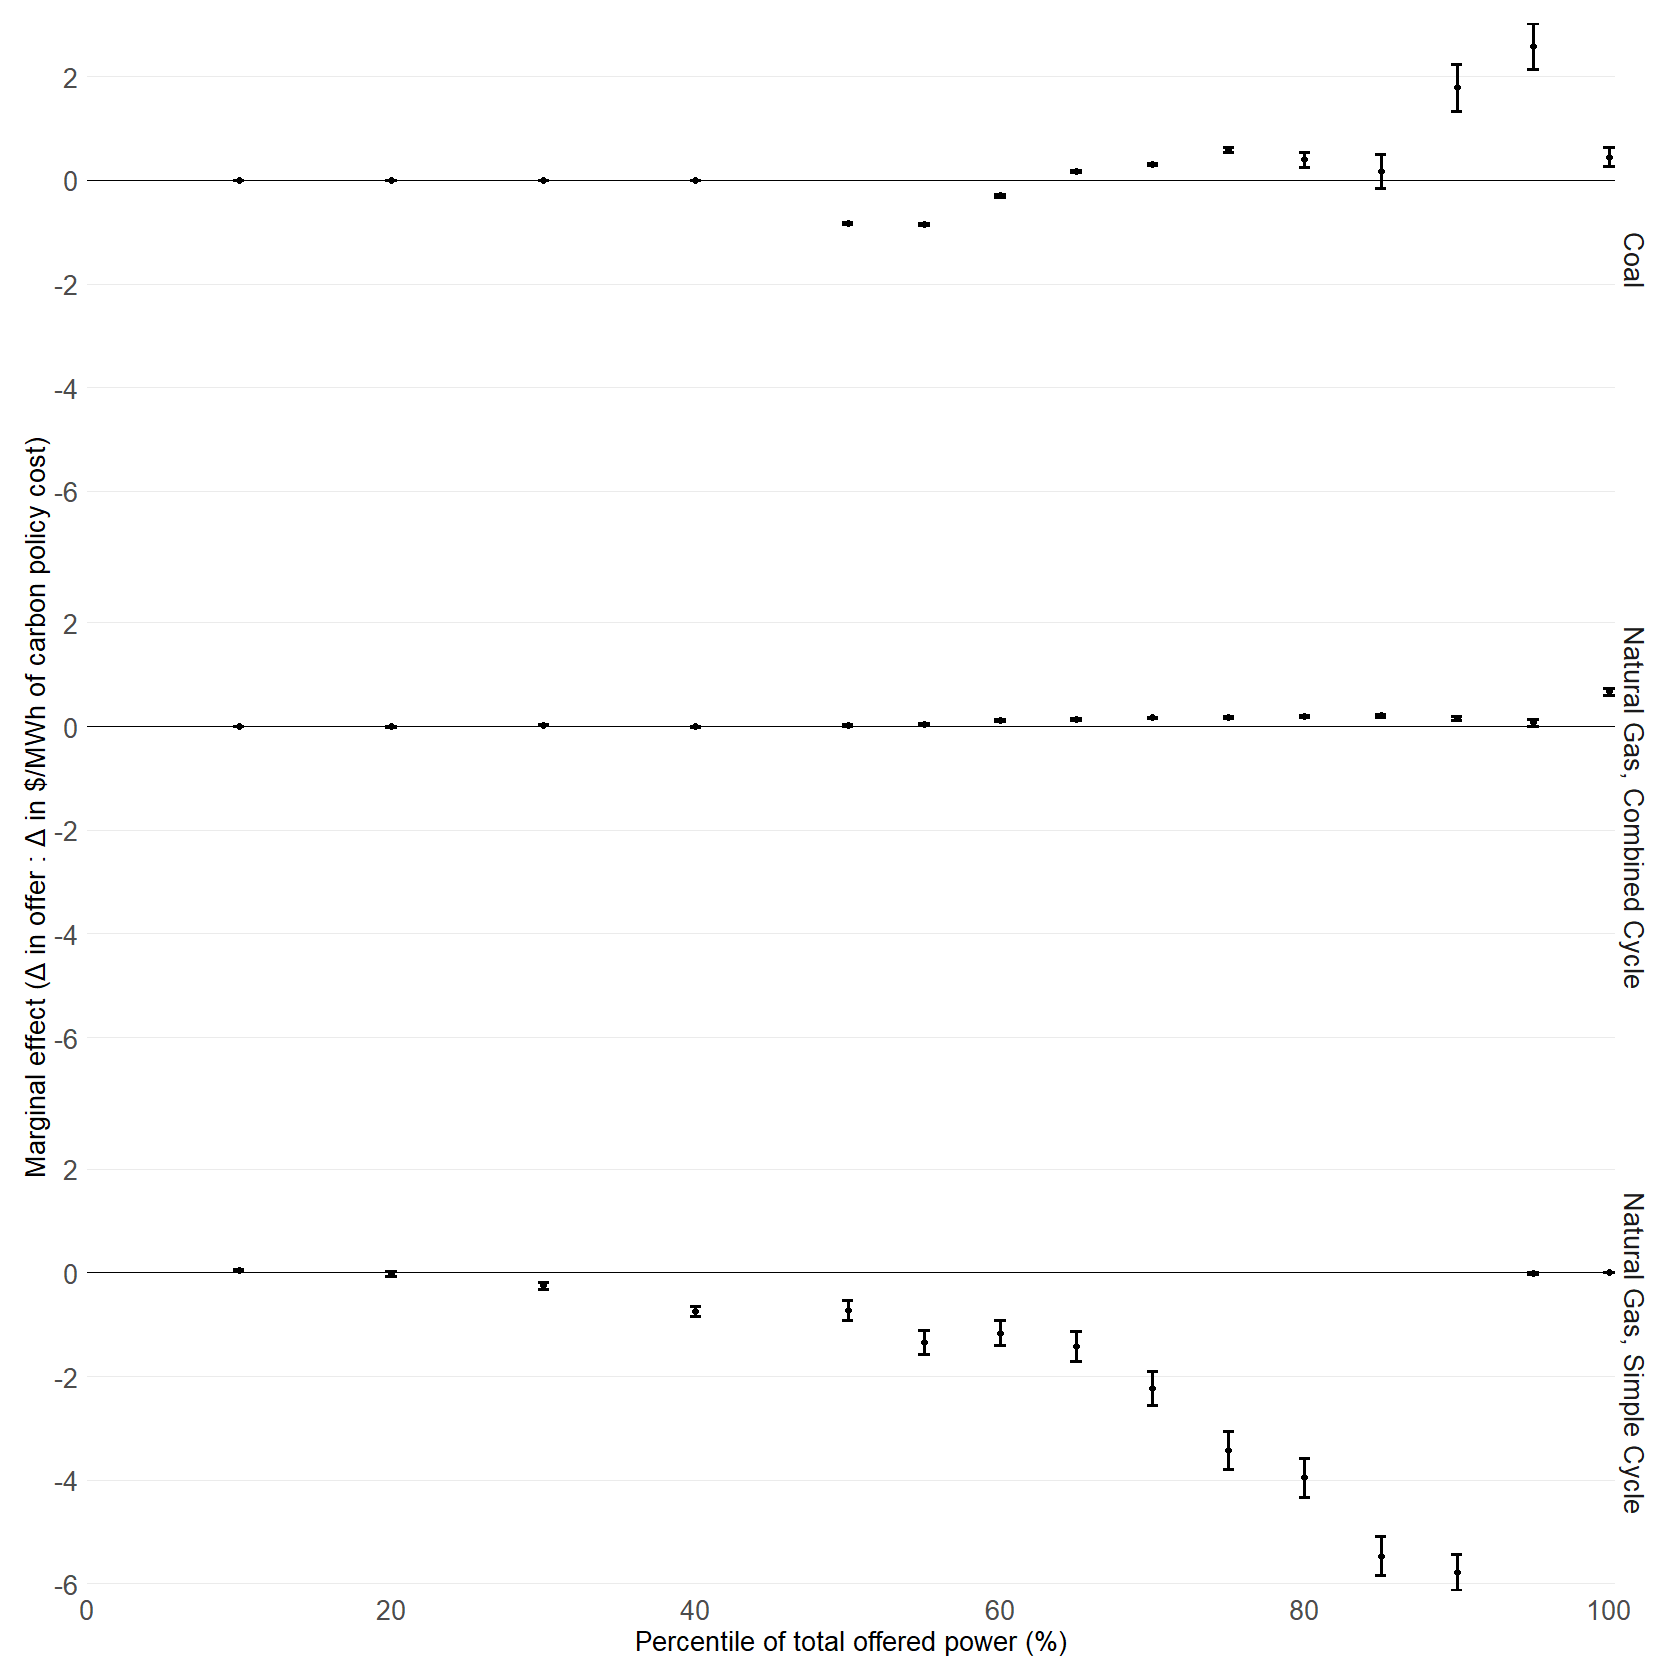
\includegraphics[width=.9\textwidth]{../images/by_type_net.png}
    \caption{Estimated marginal effect of net carbon charges on power offers, all plant types. Error bars denote 95\% confidence intervals}
    \label{fig:decomp_peaks}
\end{figure}

The natural gas, combined cycle power plants respond as we would have expected, at least qualitatively, with limited pass-through in the lower part of the merit order, where plants are generally offering in a minimum capacity at a lower strike price, an then with more pass-through in the mid- and upper-merit up to the 95th and 100th percentiles, where other strategic factors drive offers. Here, however, the quantitative effects are strikingly small. Natural gas power plants passed through less than 20\% of the net costs of carbon policies to their offers.

For the simple-cycle plants, the results are the reverse of what we might expect. For these plants, some of which operate as peaking plants, we would expect to see a near-perfect pass through or, at the very least, something similar. Instead, we see almost all sampling points in the offers from simple cycle plants showing a negative relationship with net carbon costs: higher carbon prices were equated with not only lower offers but quantitatively significant reductions in the offered price level with increases in the carbon cost.

There are a few factors at play that may explain this counter-intuitive result: first, some of the simple-cycle gas turbines are relatively new, so we do not observe all plants over the entire sample space. In and of itself, this would not be important given our sampling technique, but many of the newer simple-cycle plants have been added as a consequence of emissions policies, as alternatives to venting or flaring of methane from oil field operations. Additionally, many simple-cycle plants operate in the ancillary services market, capturing value as spinning reserves rather than when generating, and so this will skew our estimated emissions intensities since these plants would report emissions for periods in which they are burning fuel but not generating power. Finally, as coal plants have retired and/or shifted to higher offers, some simple-cycle plants would see an advantage to producing in more hours of the day, such that strategic considerations would lead them to lower their offers despite an increase in carbon costs in order to ensure a higher annual capacity factor. These plants will also be most sensitive to the hourly opportunity costs of natural gas and, while we observe hourly spot prices, individual entities may face different gas costs on an hourly basis than what we observe, in particular if facilities have long-term contracts for delivery in place.


\subsection{Impacts By Offer Control}
We can also use the data post-2013 to assess the degree to which different market participants might offer their power into the merit order and how they have passed through carbon policy values to power offers. We only use data after 2013 for this analysis because, prior to that time, the AESO did not provide offer control records along with their merit order data. The remains a sufficient sample, since we have three full years of data (2013-2015) in the initial \SGER pricing program, along with at least one full year under each of the altered policy regimes over which to assess changed in offers by different market participants.



PPA explanation...

Balancing Pool explanation...

Return of PPAs to the Balancing Pool

Declining ability to identify TransCanada impacts because of changes in resources.


\begin{figure}[!htb]
    \centering
     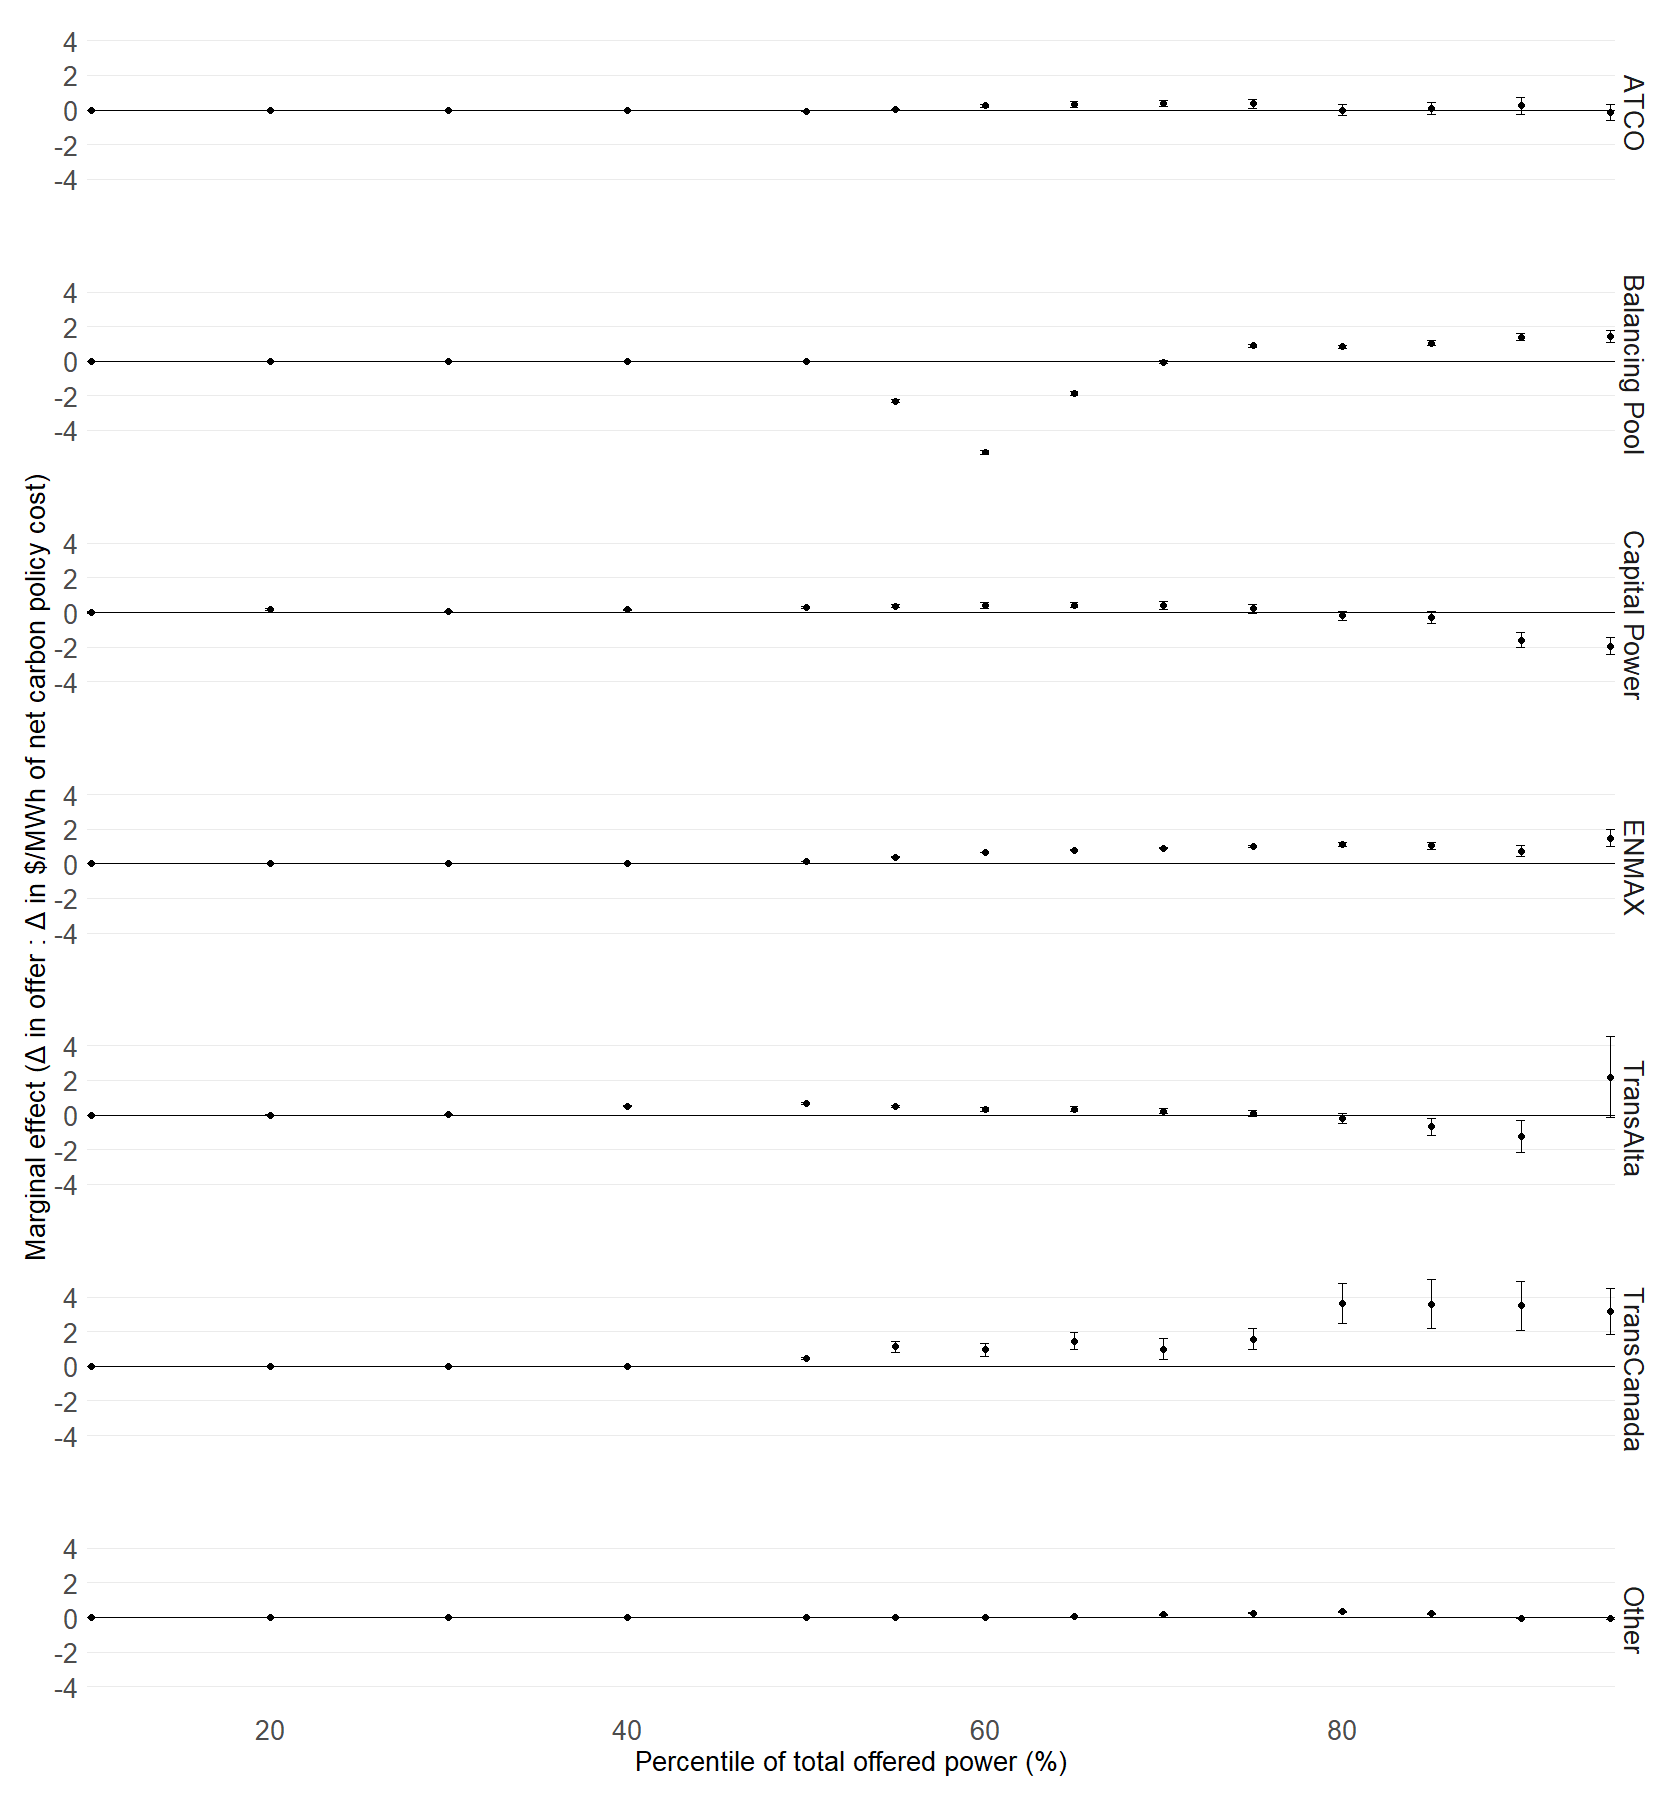
\includegraphics[width=.9\textwidth]{../images/offer.png}
    \caption{Estimated marginal effect of net carbon charges on power offers, all plant types, by controlling entity. Error bars denote 95\% confidence intervals}
    \label{fig:offer}
\end{figure}


\section{Conclusion}


\bibliographystyle{chicago}
\bibliography{../env}

\end{document}



\section{Introduction}
We examine the offer behaviour of competitive electricity suppliers in response to carbon prices. We exploit a unique set of significant policy variations over time and across facilities to measure carbon pricing pass-through to electricity prices. Beginning in 2007, the province of Alberta, Canada, instituted carbon pricing which affected generators in its energy-only wholesale electricity market. Changes in provincial governments in 2015 and 2019 led to the emissions pricing scheme being changed 3 times in 4 years, with the first 3 changes all announced during the 2015 calendar year, and a subsequent change announced in 2018. These changes were each implemented in such a way as to have firm- and facility-type-specific impacts which generates variation that we can exploit to separately characterize the role of carbon pricing and output-based allocations (OBAs) on pricing behaviour.

Compare to Mar and other literature.





First, in June 2015, it was announced that the carbon price would increase to \$20 per tonne and that output-based allocations would decrease beginning in 2016. The price was also set to increase further, to \$30 per tonne, in 2017.  Later in 2015, following the recommendations of an expert panel, the government announced that it would alter the formula by which output-based allocations were provided to one which was consistent across all electricity generators beginning in 2018. This change was material, with coal plant allocations reduced by more than 0.5t/MWh in many cases, leading to changes in average costs of output of more than \$15/MWh for some facilities.  This combination of policy changes implies that the effective marginal cost of emissions and the average emissions cost per unit output both changed significantly, with changes having different impacts on generators within and across fuel types.  We show the effect of the policy changes on average revenue by fuel type in Figure 1.

\begin{figure}[!h]%
	\centering \vspace{-.25cm} 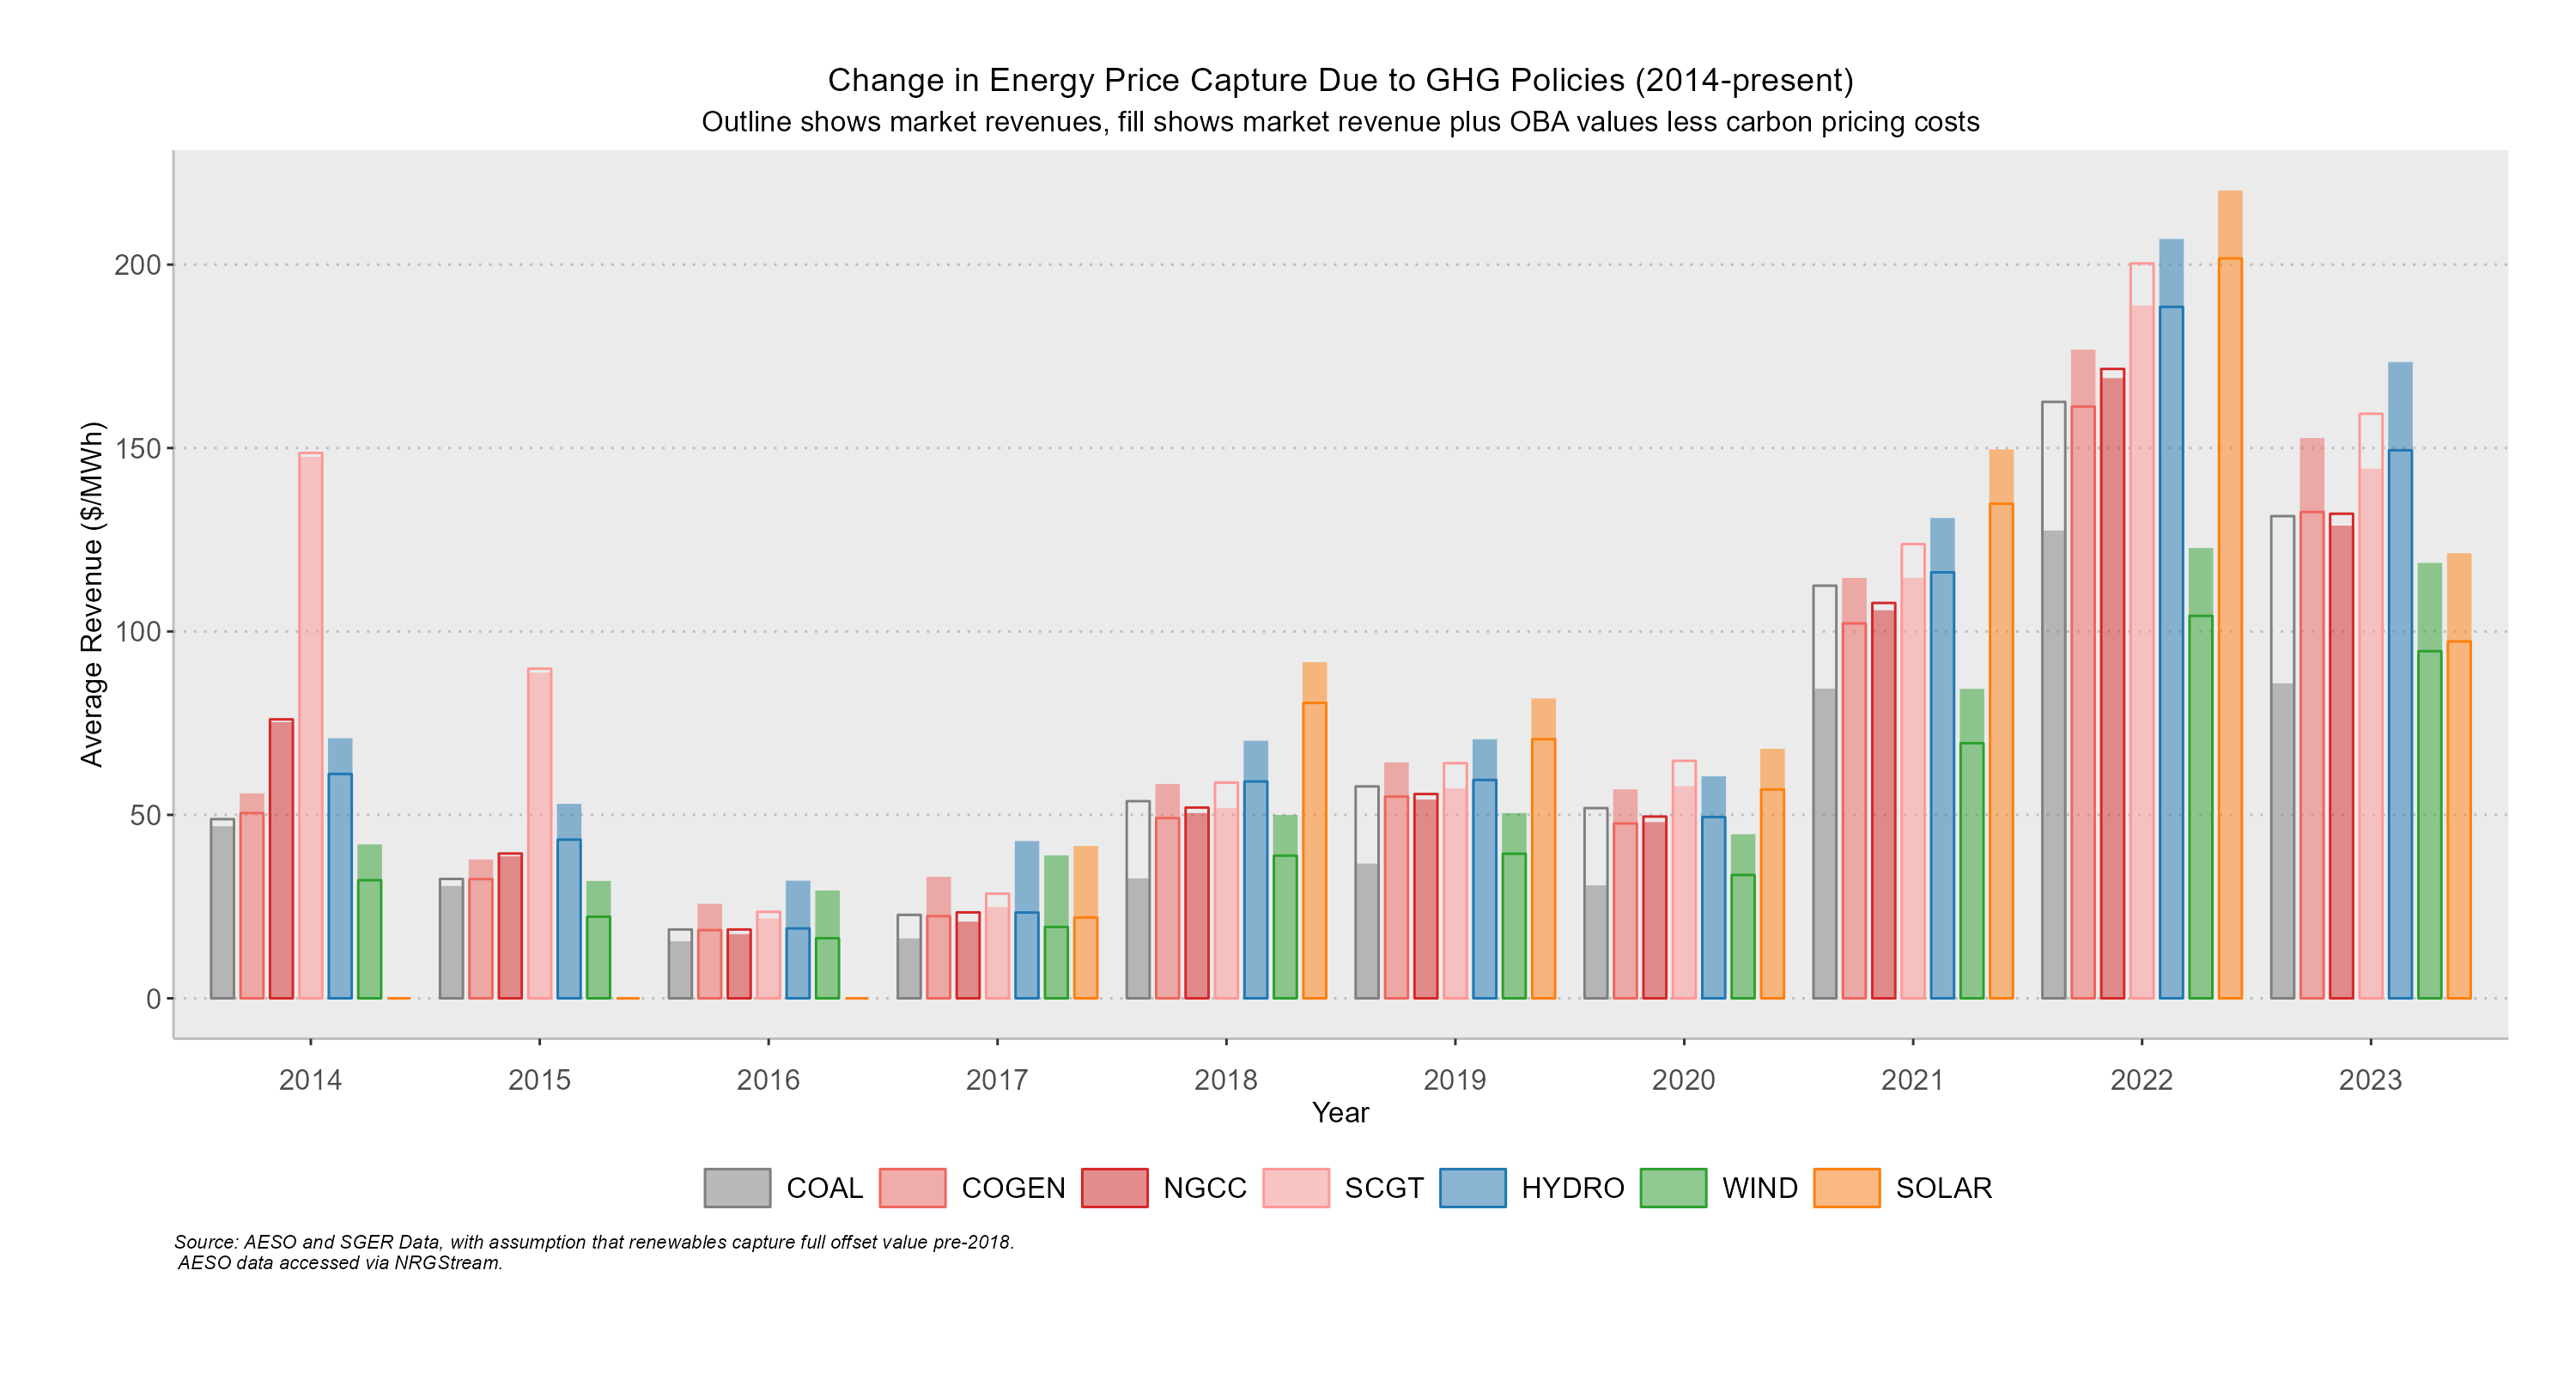
\includegraphics[width=6.5in]{../../alberta_power/price_capture_ctax.png}
\label{fig:masnadi_1}
\vspace{-0.75cm}	\caption{Impact of changes in carbon pricing on plant revenues by type}
\end{figure}


 Fossil-fuel-fired generators were charged a carbon price of \$15/tonne on emissions net of allocations of emissions credits. Emissions credits were allocated per unit output at rates based on facility-specific emissions-intensity histories. Renewable generators were also able to qualify for offset credits which provided an alternative revenue stream.

\noindent


\newpage \noindent We use data including hourly electricity prices and loads, plant availability, as well as offer functions at the plant level, historic emissions intensities, and emissions policy compliance records to assess the degree to which carbon prices have been passed through to wholesale electricity prices. We also assess the degree to which changes in the composition of the market including changes to offer control and firm concentration, as well as changes due to facility exit, have altered the pass-through of carbon prices.  Our work builds largely on the analysis of electricity price pass-through of \citet{fabra_reguant}, but also draws on work by \citet{hintermann17} on market power, \citet{hintermann15} and \citet{hintermann16} on impacts of carbon pricing in the EU-ETS, \citet{nazifi16} on pass-through in Australia's electricity market, and \citet{woo_et_al} on pass-through in California's market.

\noindent Our preliminary analysis suggests that there has been both a significant effect on emissions (see Figure \ref{fig:monthly_ghg}) and on the composition of the market (see Figure \ref{fig:monthly_gen}) with significant reduction in the generation from coal plants and significant increase in the hourly daily cycling of coal plants as the change in carbon prices push coal plants higher in the merit order relative to gas generation, a dynamic examined in \citet{cullen_mansur}.

\begin{figure}[p]%
	\centering \vspace{-.25cm} 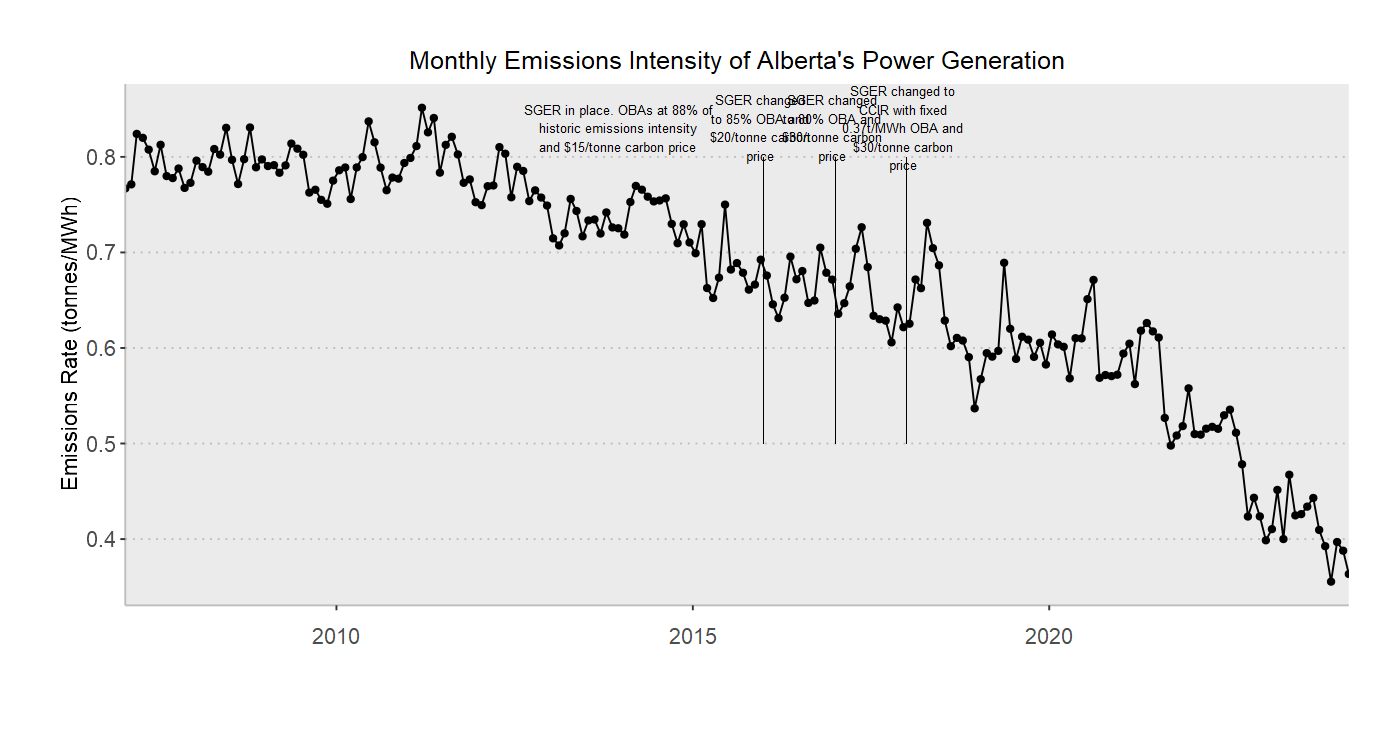
\includegraphics[width=5.5in]{../../alberta_power//monthly_ghg_mwh.png}
\vspace{-0.75cm}	\caption{Impact of changes in carbon pricing on GHG emissions}\label{fig:monthly_ghg}
\end{figure}


\begin{figure}[p]%
	\centering \vspace{-.25cm} 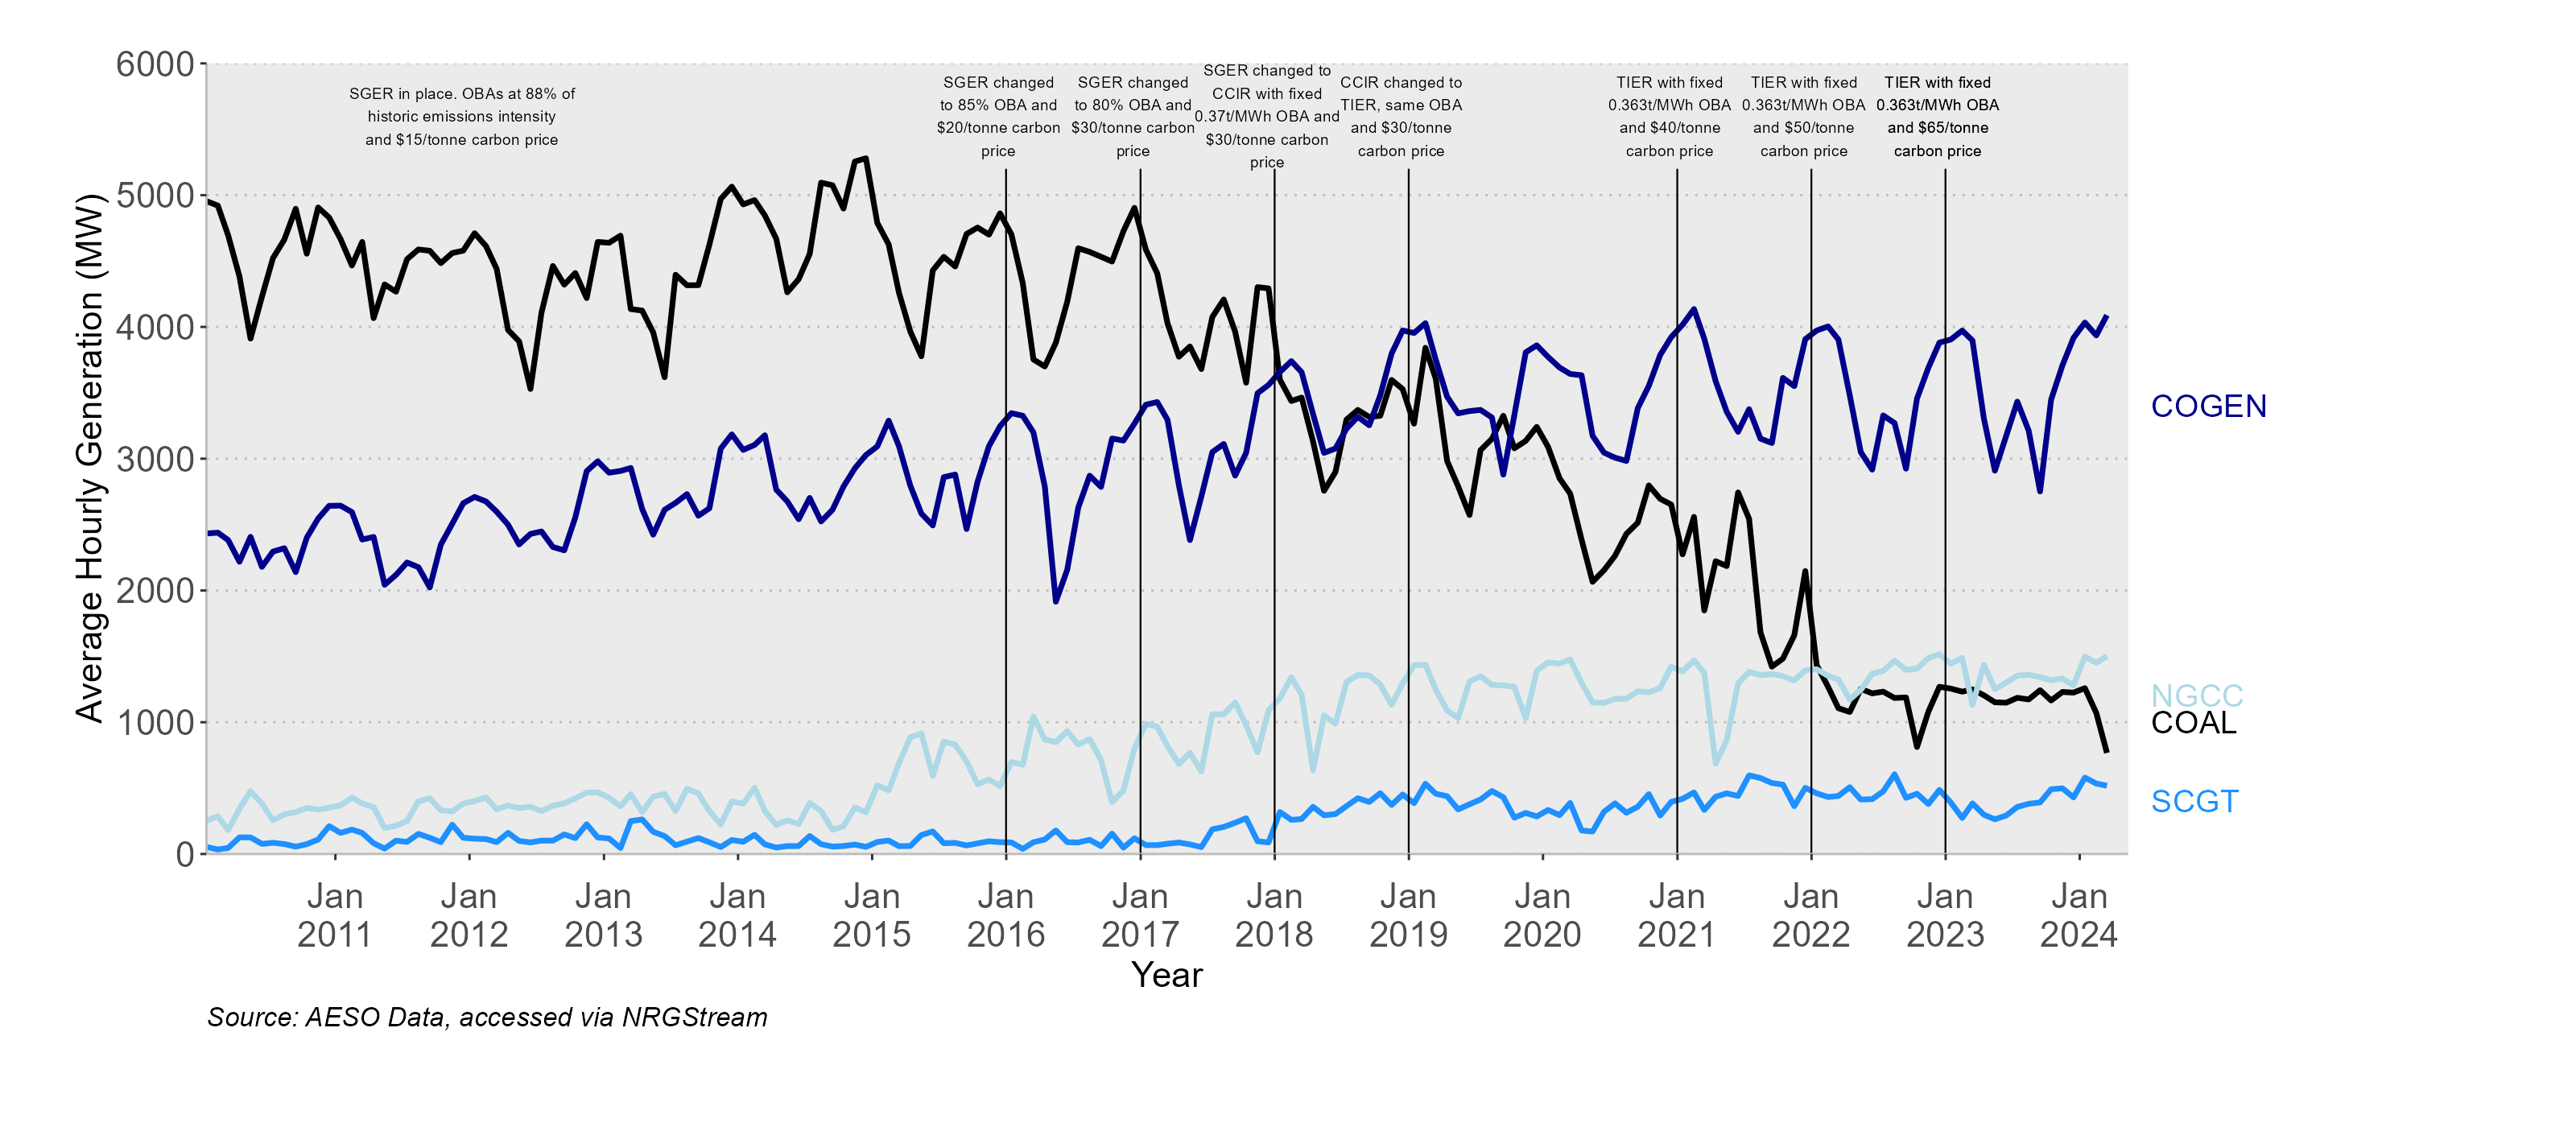
\includegraphics[width=5.5in]{../../alberta_power/gen_ghg_price.png}
\vspace{-.5cm}	\caption{Impact of changes in carbon pricing on market share by fuel. Combined heat and power (COGEN), simple-cycle gas turbines (SCGT) and natural gas combined cycle (NGCC) facilities are each natural-gas-fired.}\label{fig:monthly_gen}
\end{figure}


%\begin{figure}[!h]%
	%\centering \vspace{-.5cm} \includegraphics[width=6.5in]{CJE/masnadi_fig_1.png} %\label{fig:masnadi_1}
%	\caption{Figure 1 from Masnadi et al. (2018)}
%	\vspace{-.5cm}
%\end{figure}
\newpage
\vspace{10cm}


\begin{figure}[!h]%
	\centering \vspace{-.25cm} \includegraphics[width=6.5in]{../../alberta_power/peak_prices_2009_2019.png}
\label{fig:masnadi_1}
\vspace{-0.75cm}	\caption{Peak and off-peak power prices, 2007-2019}
\end{figure}

\newpage 